%----------------------------------------------------------------------------------------
%	PACKAGES AND OTHER DOCUMENT CONFIGURATIONS
%----------------------------------------------------------------------------------------
\documentclass[12pt, letter, oneside]{Thesis} % Paper size, default font size and one-sided paper
%\graphicspath{{Pictures/}} % Specifies the directory where pictures are stored
\usepackage{hyperref} % For internal referencing
\usepackage{lipsum} % For generating fill text for trouble-shooting LaTex
\usepackage{setspace} % For picking line spacing *within* sections
\usepackage{parskip} % For changing spacing between heads, lets me use linebreaks for spacing between paragraphs
\usepackage{float}% For Figures
	\floatstyle{plain}
	\restylefloat{figure}
	\usepackage{rotating} % For rotating figures ±90˚ use \begin{sidewaysfigure}	
%% Pick my Font
	% For Palatino
	%\usepackage[sc]{mathpazo}
	%	\linespread{1.05} % Palatino needs more leading (space between lines)
	% For Ariel
	\usepackage{helvet}
	\renewcommand{\familydefault}{\sfdefault}

% Center the Chapter and heading titles 
% http://tex.stackexchange.com/questions/23858/center-chapter-book-class
	\usepackage{titlesec}
	\titleformat{\chapter}[display]
	{\normalfont\huge\bfseries\centering}{\chaptertitlename\ \thechapter}{20pt}{\Huge}

\usepackage[T1]{fontenc} 
\usepackage{flexisym} % Lets me use prime symbols
\usepackage{gensymb} % For degree '\degree'

% For Referencing
\usepackage[square, comma, sort&compress]{natbib} 
	\setlength{\bibsep}{0.0pt} % Reduce size of bibliography
	% Use the natbib reference package - read up on this to edit the reference style; if you want text (e.g. Smith et al., 2012) for the in-text references (instead of numbers), remove 'numbers' 
% Colors hyperlinks in blue - change to black if annoying	
\hypersetup{urlcolor=blue, colorlinks=true}  

%% To highlight things for later review
\usepackage{soul} % use \hl{this is some highlighted text}

%% For Inserting Code | http://stackoverflow.com/questions/3175105/how-to-insert-code-into-a-latex-doc
\usepackage{listings}
\usepackage{color}
	\definecolor{dkgreen}{rgb}{0,0.6,0}
	\definecolor{gray}{rgb}{0.5,0.5,0.5}
	\definecolor{mauve}{rgb}{0.58,0,0.82}

	\lstset{frame=tb,
	  language=Perl,
	  aboveskip=3mm,
	  belowskip=3mm,
	  showstringspaces=false,
	  columns=flexible,
	  basicstyle={\small\ttfamily},
	  numbers=none,
	  numberstyle=\tiny\color{gray},
	  keywordstyle=\color{blue},
	  commentstyle=\color{dkgreen},
	  stringstyle=\color{mauve},
	  breaklines=true,
	  breakatwhitespace=true
	  tabsize=3
	}

\title{\ttitle} % Defines the thesis title - don't touch this
%----------------------------------------------------------------------------------------
% Organism names
%----------------------------------------------------------------------------------------
\newcommand\flies{\textit{Drosophila melanogaster}} %Done
\newcommand\locusts{\textit{Schistocerca gregaria}} % Done
\newcommand\worms{\textit{Caenorhabditis elegans}} % Done


%----------------------------------------------------------------------------------------
\begin{document}
%----------------------------------------------------------------------------------------

\frontmatter % Use roman page numbering style (i, ii, iii, iv...) for the pre-content pages
\setstretch{1.3} % Line spacing of 1.3

% Define the page headers using the FancyHdr package and set up for one-sided printing
\fancyhead{} % Clears all page headers and footers
\rhead{\thepage} % Sets the right side header to show the page number
\lhead{} % Clears the left side page header
\pagestyle{fancy} % Finally, use the "fancy" page style to implement the FancyHdr headers
\newcommand{\HRule}{\rule{\linewidth}{0.5mm}} % New command to make the lines in the title page

% PDF meta-data
\hypersetup{pdftitle={\ttitle}}
\hypersetup{pdfsubject=\subjectname}
\hypersetup{pdfauthor=\authornames}
\hypersetup{pdfkeywords=\keywordnames}

%----------------------------------------------------------------------------------------
%	TITLE PAGE Umass
%----------------------------------------------------------------------------------------
\begin{titlepage}
\begin{center}
	\huge EXAMINATION OF DYNAMIC LONG RNAS\\[2cm] 
	{\large 
		A Dissertation Presented \\[1cm]
		By \\[1cm]
		Christian K. Roy \\[1cm]
		Submitted to the Faculty of the University of the \\
		Massachusetts Graduate School of Biomedical Sciences, Worcester\\
		in partial filfillment of the requirements\\
		for the degree of \\[2cm]
		DOCTOR OF PHILOSOPHY \\[1cm]
		MAY 21st 2014\\[1cm]
		BIOCHEMISTRY\\[1cm]
 	}
 \end{center}
 \end{titlepage}
%----------------------------------------------------------------------------------------
%	Signature Page Umass
%----------------------------------------------------------------------------------------
\begin{titlepage}\label{hd:titlePage}
\begin{center}
		EXAMINATION OF DYNAMIC LONG RNAS\\[0.25cm]

		A Dissertation Presented \\[0.25cm]
		By \\[0.25cm]
		Christian K. Roy \\[0.25cm]
 
		The signatures of the Dissertation Defense Committee signify \\
		completion and approval as to style and content of the Dissertation\\[1cm]
		\rule[1em]{25em}{1pt}\\[-0.6cm]% This prints a line for the signature
		Melissa J. Moore, Co-Thesis Advisor\\[1cm]
		\rule[1em]{25em}{1pt}\\[-0.6cm]
		Phillip D. Zamore, Co-Thesis Advisor\\[1cm]
		\rule[1em]{25em}{1pt}\\[-0.6cm]
		Scot Wolfe, Member of Committee\\[1cm]
		\rule[1em]{25em}{1pt}\\[-0.6cm]
		Job Dekker, Member of Committee\\[0.25cm]
		The signature of the Chair of the Committee signifies that the written
		dissertation meets the requirements of the Dissertation Committee\\[1cm]
		\rule[1em]{25em}{1pt}\\[-0.6cm]
		Zhiping Weng, Chair of Committee\\[0.25cm]
		The signature of the Dean of the Graduate School of Biomedical Sciences signifies that the student has met all graduation requirements of the school.\\[1cm]
		\rule[1em]{25em}{1pt}\\[-0.6cm]
		Anthony Carruthers, Ph.D.,\\[0.25cm]
		Dean of the Graduate School of Biomedical Sciences\\[0.25cm]
		Biochemistry and Molecular Pharmacology\\[0.25cm]
		MAY 21st 2014 

 \end{center}
 \end{titlepage}
\clearpage % Start a new page

%----------------------------------------------------------------------------------------
%	ABSTRACT PAGE
%----------------------------------------------------------------------------------------

\addtotoc{Abstract} % Add the "Abstract" page entry to the Contents
\label{hd:abstract}
\abstract{\addtocontents{toc}{\vspace{1em}} % Add a gap in the Contents, for aesthetics

The Thesis Abstract is written here (and usually kept to just this page). The page is kept centered vertically so can expand into the blank space above the title too\ldots

}
\setcounter{page}{3}
\clearpage % Start a new page

%----------------------------------------------------------------------------------------
%	ACKNOWLEDGEMENTS
%----------------------------------------------------------------------------------------

\setstretch{1.3} % Reset the line-spacing to 1.3 for body text (if it has changed)

\acknowledgements{\addtocontents{toc}{\vspace{1em}} % Add a gap in the Contents, for aesthetics
\label{hd:acknowledgements}
First I would like to acknowledge and thank Laura Geagan and Rebecca Sendak at Genzyme. They were my supervisors while I was a research associate there, and assisted and encouraged my transition back to graduate school. Without the confidence they instilled in my abilities as a young scientist in, I doubt I would have ever signed up for more school. 

Next I’d like to thank Melissa. During my 1st year retreat at Wood’s Hole I first learned that Melissa is a fantastic communicator of interesting and important science. When she brought out her rope representing the unspliced pre-mRNA of dystrophin—a rope that reached to the back of a rather large auditorium—and then dramatically held up a No.2 pencil representing the final mRNA product, both to scale, I knew the that I wanted to do my graduate research in her lab. I have never once doubted the decision to join Melissa’s lab, and have learned so much from the broad and interconnected approach she takes to important scientific questions. Thank you so much for teaching me to always consider the big picture, go for the answer, and to just ask when I need help.

Soon after joining Melissa’s lab, and a project going well, it was proposed to me that I be a joint student between Melissa and Phil. It was not difficult to not jump at the opportunity to be advised by two Howard Hughes Investigators, and I also haven’t regretted the decision. Over the past few years, I have been continually amazed at the depth of Phil’s knowledge, in scientific and general topics. He is a careful, meticulous, quantitative, and calculating mentor. While I feel that I clicked ‘on the level’ with Melissa, interacting with Phil forced me to think and act outside my comfort zone, something I always tell myself is a critical aspect of change and growth. Thank you Phil for everything I’ve learned.

My committee has also been very supportive throughput my PhD. I hardly believed the ease with which I passed my qualifying exam, and took it as a big confidence boost. The following years of TRAC meetings confirmed that I was not thinking way off-base. The one-on-one meetings just prior to my QE were especially helpful. Thanks to Scot, Job, and especially Zhiping for all the guidance.

\begin{itemize}

  \item Lab Members;  Aaron; Alper; Amrit
  \item Eric and Erin
  \item Collaborators
  \item Dave Weaver
  \item Muro
  \item Graveley
  \item Heinrich
  \item Anna
  \item Ogo
  \item Family
  \item Jul Owen

\end{itemize}

}

\clearpage % Start a new page

%----------------------------------------------------------------------------------------
%	LIST OF CONTENTS/FIGURES/TABLES PAGES
%----------------------------------------------------------------------------------------
% The page style headers have been "empty" all this time, 
% now use the "fancy" headers as defined before to bring them back
\pagestyle{fancy} 
\lhead{\emph{Contents}} % Set the left side page header to "Contents"
	\tableofcontents % Write out the Table of Contents
\lhead{\emph{List of Figures}} % Set the left side page header to "List of Figures"
	\listoffigures % Write out the List of Figures
\lhead{\emph{List of Tables}} % Set the left side page header to "List of Tables"
	\listoftables % Write out the List of Tables
%----------------------------------------------------------------------------------------
%	ABBREVIATIONS
%----------------------------------------------------------------------------------------
\clearpage % Start a new page
\setstretch{1.5} % Set the line spacing to 1.5, this makes the following tables easier to read
\lhead{\emph{List of Abreviations}}
\label{hd:abrevs} \listAbreviations
\begin{table}[h]
\begin{tabular}{l|l}
AS       & Alternative Splicing                                 \\
DNA      & Deoxyribonucleic acid                                \\
ssDNA    & Single-stranded DNA                                  \\
RNA      & Ribonucleic acid                                     \\
ssRNA    & Single-stranded RNA                                  \\
ATP      & Adenosine triphosphate                               \\
NAD      & Nicotinamide adenine dinucleotide                    \\
ChIP-Seq & Chromatin Immunoprecipitation followed by sequencing \\
HTS      & High-throughput sequencing (see also NGS)            \\
NGS      & Next-generation sequencing                           \\
nt       & A nucleotide of either DNA or RNA                    \\
bp       & A base pair of DNA                                   \\
SRE      & Splicing Regulatory Element                          \\
IRE      & Intron Recognition Element                           \\
CNS      & Central Nervous System                               \\
TSS      & \{Transcription or Translation\} Start Site          \\
TTS      & \{Transcription or Translation\} Termination Site    \\
SAGE     & Serial Analysis of Gene Expression                   \\
\end{tabular}
\end{table}

%----------------------------------------------------------------------------------------
%	SYMBOLS
%----------------------------------------------------------------------------------------
\clearpage % Start a new page
\lhead{\emph{List of Symbols}}
\label{hd:Symbols} \listSymbols

\begin{table}[h]
\begin{tabular}{ll}
5\textprime       & The 5 prime end of a DNA or RNA molecule 			\\
3\textprime       & The 5 prime end of a DNA or RNA molecule 			\\
$\mu$       	  & Micro. A value of 1x10\textsuperscript{-6} standard units 			\\
\end{tabular}
\end{table}

%----------------------------------------------------------------------------------------
%	Definitions
%----------------------------------------------------------------------------------------
\clearpage % Start a new page
\lhead{\emph{Definitions}}
\label{hd:Definitions} \listDefinitions

\begin{description}
  \item[RNA-Seq] \hfill \\
  A technology wherein RNA is fragmented, converted to DNA, and analyzed on a high-throughput sequencing instrument
  \item[A ‘Read’] \hfill \\
  The sequence of nucleotides produced from each spot on a high-throughput sequencing machine
  \item[Insert] \hfill \\
  The RNA molecule captured between two cloning sequences in a high-throughput sequencing library preparation workflow
    \item[Read length] \hfill \\
  The number of nucleotides for each given 'read'
    \item[Read depth] \hfill \\
  The number of reads obtained from each high-throughput sequencing analysis
    \item[Coverage] \hfill \\
  A measure of the number of times each nt of a genome is sequenced. E.g. 100 million reads of a 10 million nt genome = 10X coverage, assuming uniform distribution of the 'reads'
    \item[Paired-end] \hfill \\oach1995a
  When both sides of a DNA insert or template are sequenced, utilizing the original length of DNA between the reads to facilitate mapping (\cite{Roach1995}).
    \item[Scaffold or contig] \hfill \\
  A draft sequence of nucleotides, meant to represent the actual biological sequence as closely as possible, examples include unassembled fragments of chromosomes or fragments of mRNA transcripts.
    \item[Argonaute] \hfill \\
  Protein(s) belonging to a group containing a Piwi (P-element induced wimpy testes) domain, that bind nucleic acids and participate in many target-guided processes, including RNA Interference, and RNA-indicuded transcript/gene silencing.   
\end{description}
\clearpage % Start a new page

%----------------------------------------------------------------------------------------
%	DEDICATION
%----------------------------------------------------------------------------------------
\setstretch{1.3} % Return the line spacing back to 1.3
\pagestyle{empty} % Page style needs to be empty for this page
\label{hd:Dedicatory}
\dedicatory{
	I would like to dedicate this Doctoral dissertation to my grandfather, George Knauf. My grandfather passed away on September 23rd, 2011, just one week shy of his 82nd birthday. I find it difficult to articulate how much I miss him. He spoke carefully and never without purpose or conviction. While I hear from others that he was proud of me, he rarely, if ever, betrayed that type of emotion directly. It is my goal to build as solid a life as he, founded on hard work, playing the long game, responsibility, and maintaining friendships. These are just a few of the personality traits that I observed and try to emulate. The fact that he passed before he could meet our son Owen is one of my biggest regrets. Of all the possessions he left behind, it is the memory of our time together that I will cherish the most. Rest in peace, Grump. I did it. 
} % Dedication text
\addtocontents{toc}{\vspace{2em}} % Add a gap in the Contents, for aesthetics
\clearpage % Start a new page

%----------------------------------------------------------------------------------------
%	Preface
%----------------------------------------------------------------------------------------

\prefaceSection

The work reported in this dissertation has been published in the following articles.
Chapter \ref{Chapter4} has been published previously as:\\
Li, X. Z. Z., Roy, C. K. K., Dong, X., Bolcun-Filas, E., Wang, J., Han, B. W. W., … Zamore, P. D. D. (2013). An Ancient Transcription Factor Initiates the Burst of piRNA Production during Early Meiosis in Mouse Testes. Molecular Cell, 50(1), 1–15. doi:10.1016/j.molcel.2013.02.016

Some contents of Chapter \ref{Chapter3} are included in a currently submitted manuscript. 

\clearpage

%----------------------------------------------------------------------------------------
%	THESIS CONTENT - CHAPTERS
%----------------------------------------------------------------------------------------

\mainmatter % Begin numeric (1,2,3...) page numbering
\pagestyle{fancy} % Return the page headers back to the "fancy" style
%\setstretch{2} % Line spacing of 2
\setstretch{1} % Line spacing of 1
\label{hd:Chatpers}
% My Thesis Introduction
% 2014-03-25
% Christian Roy
\chapter{Introduction} % Main chapter title
\label{Chapter1} % To refernce this chapter elsewhere, use \ref{ChapterX}
\lhead{Chapter 1. \emph{Introduction}} % Change X to a consecutive number
% this is for the header on each page - perhaps a shortened title
%----------------------------------------------------------------------------------------

%% gene names
\label{geneNames}
\newcommand\slo{\textit{slo1}}
\newcommand\fn{\textit{Fn1}}
\newcommand\kcnma{\textit{Kcnma}}
\newcommand\dscam{\textit{Dscam1}}

%----------------------------------------------------------------------------------------
%	SECTION 1
\section{On the importance of gene expression}\label{sec:Importatance of Gene Expression} 
%----------------------------------------------------------------------------------------

Exodus tells of the liberation of the Israelites from Egyptian slavery. Humble and reluctant Moses, their divine-apointed leader, attempts to force the Pharaoh Ramses to release the Israelites through infliction of a series of 10 plagues. Pharaoh is stalwart and stubborn through plauges that turn water to blood, flood the streets with frogs, lice, and flies. Even as livestock fell dead from disease, people and animals both are covered in boils, and the land burns in storms of fire, Pharaoh does not bend.

The 8th plague was a swarm of Locusts, described in Exodus 10: 14–15:

\begin{quote}
	\itshape % This will be italicized quote
	\singlespacing
	\textsuperscript{14} And the locusts went up over all the land of Egypt, and rested in all the coasts of Egypt: very grievous were they; before them there were no such locusts as they, neither after them shall be such.\\
	\textsuperscript{15} For they covered the face of the whole earth, so that the land was darkened; and they did eat every herb of the land, and all the fruit of the trees which the hail had left: and there remained not any green thing in the trees, or in the herbs of the field, through all the land of Egypt.
\end{quote}

The desolation left by the locust plague was still not enough to persuade Ramses. Nor was three days of darkness. Only the death of all first-born Egyptians, included Ramses own son, was enough to persuade Pharaoh to liberate the Israelites.

The power of a locust swarm is not just a fanciful biblical story, and is perhaps the most \textit{believable} of the 10 plagues. In current times, the United Nations' (UN) Food and Agriculture division maintains a \href{http://www.fao.org/ag/locusts/en/info/info/news/index.html}{Locust watch website} providing weekly updates on potential locust swarms in northern Africa and the Middle East. Locusts have long been, and continues to be, a powerful and feared force of Nature.

Unlike fire and brimstone from the heavens, locusts are something that can be observed and studied. What triggers them to swam and cause massive destruction? We know that the desert locust, \locusts{}, is the one of 10 others species that swarm and cause massive crop damage. \locusts{} are in the insect Order Orthoptera, along with crickets and katydids. Orthoptern members make sound known as \textit{stridulation} by vigorously rubbing their wings, making for a noisy cloud of devastation.

%They also undergo incomplete metamorphosis (formally Hemimetabolism), and do not have a pupal stage during development. \locusts{}

%% ############# FIGURE
\begin{figure}[htbp]
	\centering 
	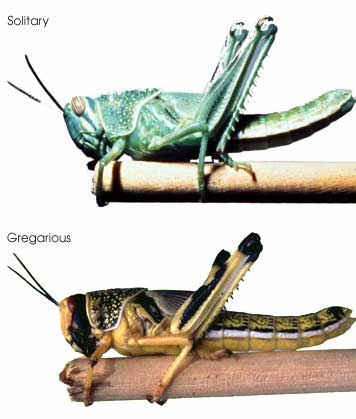
\includegraphics{Figures/Chapter1/DesertLocust.jpeg}
	\caption[The Solitary and Gregarious forms of \locusts{}]
	{
		The Solitary and Gregarious forms of \locusts{}\\[0.25cm]
		The two phenotypic forms of Schistocerca gregaria appear very different.  The Solitary form is green an generally larger, while its gregarious form is more brightly colored, smaller, and capable of swarming in vast numbers, destroying crops vegetation. Photo from \href{http://www.wikicommons.com}{Wikicommons}.
	}
	\label{fig:Locust}
\end{figure}
%% ############# FIGURE

A Desert Locust only weighs 0.05\textendash 0.07 ounces, and is less than 2.5 inches long. They can consume their own body weight in vegetation per day. One \href{http://animaldiversity.ummz.umich.edu/site/accounts/information/Melanoplus_spretus.html}{swarm} of the infamous, and now curiously extinct, Rocky Mountain locust contained 12.2 trillion insects, weighed 27.5 million tons, covered almost 200 square miles (2/3 the size of ), and could travel 60 miles in a day. A locust swarm is truely a modern biblical plague.

By definition swarms are temporary; the movement, en masse, from one
 location to another. Where do 12.2 trillion locusts go when not swarming? Does anyone care if their crops aren't under assault? It seemed no one cared enough, until about 1921, when an important realization was made.

 The power and destruction \locusts{} can inflict makes it difficult to believe that they are nothing more than common grasshoppers. Nothing more than grasshoppers not just by analogy, but by actual \textit{Taxonomy}. Desert locusts are actually the \textit{gregarious} form  of \locusts{} (See Figure ~\ref{fig:Locust}), while the more familiar and docile looking grasshopper is the \textit{solitary form}. What makes it possible for such a dichotomy to exist within the same organism, indeed the same \textit{genome}, is just now beginning to be understood.

\locusts{} are \textit{polyphenic}, meaning that they have multiple (poly) physical forms (phenotypes). Polyphenism is a general feature among insects. Phenotypes are often extremely different. For example, pea aphids (\textit{Acyrthosiphon pisum}), which usually exist in an asexually reproducing, wingless female form, respond to reduced food supply overcrowding by producing winged offspring. Winged organisms travel to new sources of food and revert back to the asexually reproducing form \citep{Shingleton2003,Purandare2014b}. In the case of \locusts{}, phenotyically the gregarious form is smaller and more brightly colored compared to its solarity cousins. This transformation can happen in as little as two hours. What is the underlying cause of this transformation?

In 2009, \citet{Anstey2009} reported that in just two hours after forced crowding of \locusts{}, elevated levels of the neurotransmitter serotonin could be detected in the gangilia (brain). These levels were strongly correlated gregarious form indicators.
% Now lead into refs 29 % 30 of Anstey2009 that talk about serotinin-induced gene changes.
\citep{Anstey2009}

% Finish with a transition about the power and complexity of DNA.
In an extremely interesting \href{http://aeon.co/magazine/nature-and-cosmos/why-its-time-to-lay-the-selfish-gene-to-rest/}{article}, David Dobbs compares the two forms of \locusts{} to that of Dr Jekyll and Mr. Hyde, the principle characters of Robert Louis Stevenson novella. For Dr Jekyll in fiction, and for \locusts{} in reality, the power to morph into multiple forms demonsrates the incredible power and plastic nature of gene expression. 

%----------------------------------------------------------------------------------------
%	SECTION 1
\section{Nucleic Acid Sequencing}
%----------------------------------------------------------------------------------------
\subsection{DNA Sequencing History} %	SUBSECTION 1
%----------------------------------------------------------------------------------------

Soon after it was realized that DNA is the source of genetic information in all living organisms \citep{Watson1953a}, and the \textit{pretty} and \textit{elegant} arrangement of complementary, antiparrallel DNA strands, was known \citep{Watson2012a}, the ability to determine specific arrangements of nucleotide bases (i.e. to sequence) in a given length of DNA was seen as a critical missing piece of technology. It took 25 years after the nature of DNA's architecture to be able to determine the specific arrangement of nucleotides in the polymer\textemdash to sequence it. By 1977, two completely different methods developed by Sanger \citep{Sanger1975a,Sanger1977b} and Maxam-Gilbert \citep{Maxam1977a} were reported. These sequencing technologies, from then on referred to eponymously as ‘Sanger’ or ‘Maxam-Gilbert’ sequencing, were used to determine the specific order of a small piece of DNA (200–300 nt). Sanger sequencing soon dominated most sequencing reactions, likely due to the conceptually more intuitive nature of the technology, and over the past 35 years, DNA sequences have been slowly cloned, sequenced, analyzed, and dutifully cataloged into knowledge.

During the late 1970’s and throughout the 1980’s, DNA sequences were typically communicated in important publications \citep{Cordell1980a,Sanger1978a}. The birth of the Internet in the 1990’s made essential publically-funded repositories for sequence information easily available \citep{Benson2011a}. However, it was the human genome project \citep{Lander2011a,Venter2001}, that provided the important activation energy that brought DNA sequencing from a hard-to-perform, but necessary, analysis, to an organized large-scale effort of assembling the complete genetic material complex genomes. An often criticized, but undeniably disrupting force in the human genome project was the competing efforts of the privately-owned company Celera \citep{Venter2008a}. Taking a higher-throughput and centralized approach to determining the sequence of the human genome, Celera fundamentally changed the landscape of genome assembly. Instead of assigning specific sections of the genome to be worked out by individual labs, Celera parallelized the effort, by collecting many of the best “high-throughput” Sanger-sequencing devices from Agilent (ABI 3700 DNA Analyzer). Using "shotgun" approach \citep{Staden1979}, sequenced pairwise \citep{Roach1995}, and combined with sequence scaffolds made available by the publicly-funded project, Celera was able to assemble high-quality genomic sequences very quickly. Arguably, this was the first deep sequencing effort, and changed the landscape of molecular and biochemical research, coincident with the beginning of a new millennium.

%----------------------------------------------------------------------------------------
\subsection{History of High-throughput Sequencing}
%----------------------------------------------------------------------------------------

Sequencing DNA by Sanger’s technology remains a valuable and critical tool in every biological scientist’s arsenal. However, the technology has a practical throughput limit. Each DNA molecule to be sequenced must be isolated and clonally amplified, typically using bacteria. Given that the human genome \citep{Hattori2005a} comprises > 3 billion nt (on just one strand), and that each Sanger reaction will provide ~800nt of quality sequence, we need at least ~4 million individual reactions to determine the sequence of the human genome, assuming that all of our reads are of sufficient quality, length, and do not overlap by even 1 nt. Even the best practical improvements to work-flows could not bring the Sanger approach to DNA sequencing in-line with aspirations of analyzing genomes of many different species or individual organisms.

In the early 2000’s, efforts to change the approach to DNA sequencing, first using MPSS \citep{Brenner2000a}, but perhaps more importantly, by Pyrosequencing \citep{Ronaghi1998a} and Polony sequencing \citep{Shendure2005}. Both of the latter methods utilize emulsion PCR \citep{Nakano2003a} for clonal amplification prior to sequencing, removing the bottleneck of bacterial cloning. In contrast to Sanger sequencing, where the signal is from fluorescence of the last incorporated chain-terminating nucleotide, Pyrosequencing visualizes light given off by luciferase as it reacts with ATP generated from the pyrophosphate (PPi) by-product of nucleotide addition. Pyrosequencing has been commercialized by 454 technologies. Polony sequencing involves a more complicated sequencing-by-ligation method, eventually commercialized by Applied Biosystems and branded as SOLiD sequencing. While both of these technologies provided valuable, high-throughput sequences, neither has been as successful as the approach commercialized by Solexa, eventually purchased and now known as Illumina.
Illumina uses a sequencing-by-synthesis approach using fluorescent nucleotides after clonal amplification of DNA on a slide surface \citep{Bentley2008}. Since 2006, iterations of the Illumina platform (eg. GE, GE-II(x), Hi-Seq, Hi-Seq 2500) have demonstrated a steady and impressive increases in both read depth and length. On February 15th 2012, Illumina announced on its \href{http://blog.basespace.illumina.com/}{Basespace blog}, that they had sequenced a HapMap sample at 40X coverage, using the HiSeq 2500 platform and paired-end 100 nt reads in a single run. This announcement demonstrated that in a single analysis attempt (but certainly not the day claimed by the title), analysis and assembly of a human genome is no longer the monumental endeavor it once was, and that completely new experimental possibilities are a reality for life science research.

%% ############# FIGURE
\begin{figure}[htbp]
	\centering 
	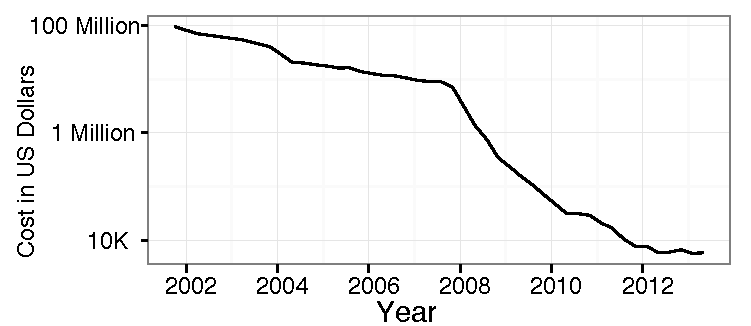
\includegraphics{Figures/Chapter1/Sequencing_costs_over_time.pdf}
	\caption[Cost of sequencing the human genome over time]
	{
		Cost of sequencing the human genome over time\\[0.25cm]
		The costs of sequencing the human genome has decreased on a log scale over a roughly 10 year period thanks 
		to major improvements in high-throughput sequencing. Data from Wetterstrand KA. DNA Sequencing Costs: 
		Data from the NHGRI Genome Sequencing Program (GSP) Available at: \url{www.genome.gov/sequencingcosts}. Accessed 2013-09-03).
	}
	\label{fig:SeqCosts}
\end{figure}
%% ############# FIGURE

%----------------------------------------------------------------------------------------
\subsection{Deep-sequencing RNA methodologies}
%----------------------------------------------------------------------------------------

%Just found the mother load of literature reviews http://blog.sbgenomics.com/history-of-rna-seq/ 

%Also this appears to be a recent (but not great) review about transcriptome analysis using RNA-Seq (Mutz et al. 2013)

%<History> - start with a simple history of splicing, mention 

The first widely-accepted method for measuring gene expression via sequencing by proxy of cDNA molecules was Serial Analysis of Gene Expression (SAGE) \citep{Velculescu1995a}. While the importance of microarrays in the measurement of gene expression via cannot be overstated \citep{Shendure2008,Marioni2008} the technologies limited ability to investigate novel sequences, and analogue signal, makes their relevance to this section somewhat off-topic. However, SAGE, (similar to the previously discussed MPSS technique) produces a digital output of gene expression using a cleaver procedure of cleaving cDNA molecules using restriction endonucleases that leaves a sticky end. After cleavage, these molecules are ligated and concatenated together to form longer DNA fragments. Fragments are cloned into a vector, amplified, and Sanger sequenced. Using known sequences incorporated during concatenation, the number of sequenced 'fragments' that align to a given gene is related to the abundance of the original mRNA molecule. While SAGE was a cleaver molecular trick allowing researches to dip into the 5-log range of expression typically seen in mRNA expression, it is still limited by read lengths and practical read depth of Sanger sequencing. 

Not long after the Solexa/Illumina platform produced read lengths of sufficient length of depth to consider measuring gene expression were the first RNA-Seq papers published \citep{Mortazavi2008, Nagalakshmi2008,Lister2008}. These papers gave a powerful glimpse into the future of molecular biology. Indeed, in the years since, analysis by RNA-Seq has quickly overtaken other forms of gene expression analysis, as demonstrated by the number of accessions deposited in GEO per year \citep{Barrett2013}. RNA-Seq allows for digital quantification of RNA expression across physiologically-relevant ranges \citep{Blencowe2009}. While simultaneously measuring gene expression, the data can be used for novel sequence discovery, measuring RNA-editing \citep{Li2011}, transcript assembly \citep{Trapnell2010}. By modifying the basic protocol or performing additional biochemical steps, RNA-Seq can be used to investigate many aspects of RNA biology (see \ref{fig:htsMethods}). 

%% ############# FIGURE
\begin{figure}[htbp]
	\centering 
	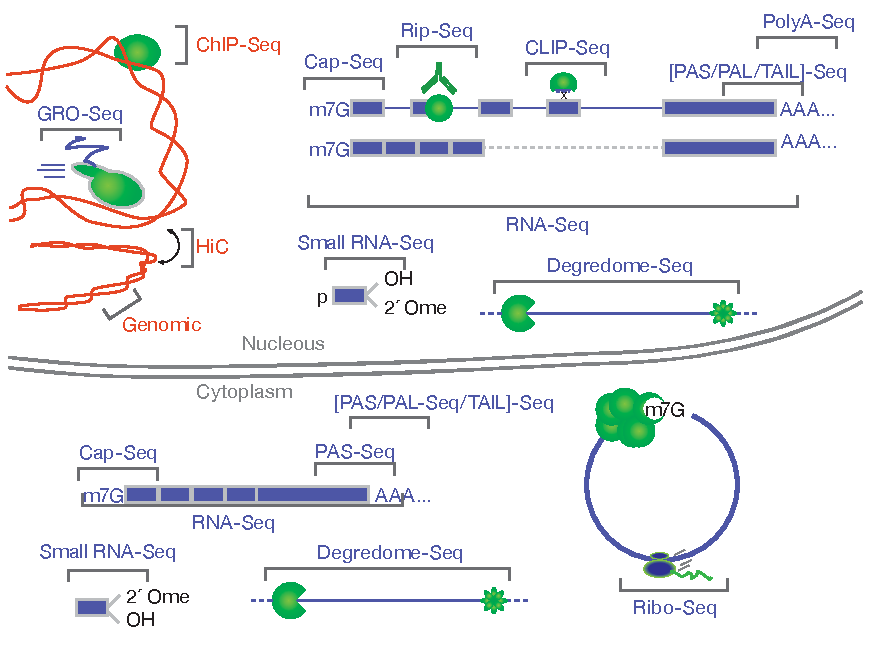
\includegraphics{Figures/Chapter1/RNA_Sequencing_methodologies.pdf}
	\caption[Methods for High-throughput sequencing of RNA]
	{
		Methods for High-throughput sequencing of RNA\\[0.25cm]
		In the short years since the first report of RNA-Seq, many variations have been reported. The figure above provides an incomplete graphical illustration of some of these variations. A more complete list of *Seq applications is maintained on this \href{http://liorpachter.wordpress.com/seq/}{blog}.
	}
	\label{fig:htsMethods}
\end{figure}
%% ############# FIGURE

RNA processing begins the moment the nascent RNA is exposed from the polymerase exit channel. Many methodologies have been developed that enrich RNA-Seq libraries for RNA molecules. For example, measurement of nascently transcribed RNA can be performed via GRO-Seq \citep{Core2008a}. Measuring the extremely complicated process of RNA turnover (referring to the rates at which RNAs both are produced and degraded) \citep{Ghosh2010a}, can be done using XXX-Seq after incorporation of XX nucleotides or a biochemical handle such as biotin. 
% cite Geisberg2014? Global Analysis of mRNA Isoform Half-Lives Reveals Stabilizing and Destabilizing Elements in Yeast  
RNA::protein interactions can be measured with or without cross-linking the protein to the RNA, via CLIP or RIP, respectively. Once an RNA has been fully transcribed, known processing steps such as Cap formation and poly(A) tail formation can be measured using any of the Cap-Seq/CAGE methodologies \citep{Shiraki2003a}, or PAS-Seq \citep{Shepard2011}. With appropriate size-selection steps, small RNAs \citep{Ghildiyal2008} can also be captured into a sequencing library. Finally, traditional RNA-Seq, can effectively capture fragments of all of the above mentioned libraries, even though it is mainly associated with measurement or analysis of traditional mRNAs.

%<Need to add PAL-Seq to the figure below> See Paper Phil sent out from the Burge lab.
%<Also we have TAIL-Seq from the Kim Lab> 
%Chang, Hyeshik, Jaechul Lim, Minju Ha, and V. Narry Kim. 2014. “TAIL-Seq: Genome-Wide Determination of Poly(A) Tail Length and 3\textprime~ End Modifications.” Molecular Cell (February): 1–9. doi:10.1016/j.molcel.2014.02.007. http://linkinghub.elsevier.com/retrieve/pii/S109727651400121X.
%Subtelny, Alexander O., Stephen W. Eichhorn, Grace R. Chen, Hazel Sive, and David P. Bartel. 2014. “Poly(A)-Tail Profiling Reveals an Embryonic Switch in Translational Control.” Nature (January 29). doi:10.1038/nature13007. http://www.nature.com/doifinder/10.1038/nature13007.

RNA-Seq and its associated flavors are also traditionally associated with measuring gene expression in tissue culture cells, or RNA extracted from particular tissues. Recently, efforts to measure the RNA expression occurring in individual cells has gained attention \citep{Shapiro2013b}. Perhaps the most interesting concept when thinking about measurement of gene expression in a single cell is the \underline{biological uncertainty principle}, wherein it is possible to either know, or change \textemdash but not both \textemdash the RNA composition of a single cell. The name borrows from Heisenberg's uncertainty principle \citep{Kennard1927} and is often confused with the more appropriate ‘observed effect’ \citep{Riley2013}. Leaving that issue aside, measuring the unique transcriptome of a given cell amoung cells of a common tissue is an exciting and informative endeavor \citep{Shalek2013b,Wills2013}. Compared to DNA, the diversity of RNA synthesis within living cells is potentially much more complicated \citep{Shendure2012}, and the ability to accurately measure RNA dynamics should allow us to make much more informative observations concerning biology then is currently possible \citep{Djebali2012}.

%Include this Recent citation for single-cell RNA-Seq versus cell pools
%Marinov, Georgi K, Brian a Williams, Kenneth McCue, Gary P Schroth, Jason Gertz, Richard M Myers, and Barbara J Wold. 2013. “From Single-Cell to Cell-Pool Transcriptomes: Stochasticity in Gene Expression and RNA Splicing.” Genome Research (December 3): 496–510. doi:10.1101/gr.161034.113. http://www.ncbi.nlm.nih.gov/pubmed/24299736.

%----------------------------------------------------------------------------------------
\subsection{Measuing RNA Expression via Sequencing}
%----------------------------------------------------------------------------------------

% Here you need to talk about the Encode paper, which you left off with in the last section

The encode project revealed that most of the genome is transcribed into RNA. This was done in cancerous cell lines, and while it revealed the potential for transcription, it did not reveal much biology beyond cells in culture simply perpetuating their existence. 

%----------------------------------------------------------------------------------------
\section{Nucleic Acid Splicing}
%----------------------------------------------------------------------------------------
\subsection{Alternative Splicing}
%----------------------------------------------------------------------------------------

% See this Review for good information 
	% \citep{Kelemen2013}

% There is a AG dinucleotide exlusion zone between the brand point and 3\textprime~ SS in Ased exons 
	% \citep{Gooding2006}

% Mention the pair of papers in science, dec 2012 that discuss evolution using RNA-Seq 
	% citep{Barbosa-Morais2012,Merkin2012} 

% Add a section about long genes/transcripts? 
	% New papers discussing importance of topoisomerase just came out in Nature - 
	% King2013. “Topoisomerases Facilitate Transcription of Long Genes Linked to Autism.”

% Figure Idea
% You already have a figure like this - comparing genome size to percent alternatively spliced *predictions* overtime for humans.  This would be a take on *organism complexity* vs *percent AS*
% + Percentage of AS for organisms in increasing complexity
     + See the chapter 4 of the Spliceosomal pre-mRNA splicing book. 2014

     + Yeast
     + Caenorhabditis elegans  is 25% Ramani AK, Calarco JA, Pan Q et al (2011) Genome-wide analysis of alternative splicing in Caenorhabditis elegans . Genome Res 21: 
     342–348
%    + Flies are 60.7%
%     + Humans are 95%

Soon after the discovery of introns, it was reasoned that genes could be arranged in different combinations, greatly increasing the coding potential of a genome \citep{Gilbert1978a}. The process of rearranging genes, now known as alternative splicing (AS), has proven to be an integral phase of gene expression in most eukaryotes. In just 15 years, the number of genes estimated to be alternatively spliced has grown considerably. Phillip Sharp, Co-Nobel-prize winner for the discovery of splicing, stated that: “Approximately, one of every twenty genes is expressed by alternative pathways of RNA splicing in different cell types or growth states” \cite{Sharp2014}. Not long after the assembly of the first human genome, a number of groups combed through Expressed Sequence Tag (EST) databases to increase that estimate to 35\%-59\% \citep{Modrek2002}. Soon after, analysis using specially designed microarrays resulted in an increased estimate of 74\% \citep{Johnson2003}. However, in late 2008, three groups utilizing high-throughput sequencing (HTS) of cDNA (referred to as RNA-Seq) demonstrated that between 86\% and 95\% of human multi-exon genes are subject to AS \citep{Pan2008, Wang2008, Sultan2008}. Not only did they demonstrate that almost all genes are alternatively spliced, they also showed that AS often occurs in a tissue- and cell type-specific manner. In combination with regulation of transcription itself, the study of AS is critical to our understanding of the connections between the comparably static genomic DNA sequence and the highly flexible and adaptive abilities of organisms.

%----------------------------------------------------------------------------------------
\subsection{Deciphering a splicing code}
%----------------------------------------------------------------------------------------

A gene is alternatively spliced when, as a result of transcription and processing, there are at least two unique transcripts produced from one genomic sequence. Beyond counting observed isoforms, one major area of effort is to decode sequence regulatory elements (SREs) contained in pre-mRNA that define AS site selection \citep{Wang2008}. In contrast to the core splicing signals, we have limited knowledge of the SREs that serve to increase, or decrease, the strength of a particular splice site, often within a sea of other potential sites. Through a variety of mechanisms, these elements serve as cis-acting sequences and binding sites for trans-acting factors. Some of the best-studied SREs include Exon Splicing Enhancers and Silencers (ESEs and ESSs). Members of the Serine-Arginine (SR) protein family typically bind to ESEs located in an exon, promoting its definition and thereby increasing the probability that the exon will be included in the final transcript \citep{Graveley2000,Long2009}. Meanwhile, ESSs serve to squelch inclusion, often through binding trans-acting heterogeneous ribonucleoprotein particles (hnRNPs) \citep{Martinez-Contreras2007}. Therefore, binding of these trans-acting factors to their appropriate SREs can either promote or inhibit interactions between the splicing machinery and the pre-mRNA. The current working hypothesis is that a finely tuned combination of these binding events determines the final exon content of each isoform \citep{House2008}. 

Sequence motifs that compose the AS code have been teased out \citep{Ladd2002, Barash2010}. Additionally, assignment of the binding motifs to tissue-specific trans-acting factors has also progressed \citep{Jin2003,Ule2005,Licatalosi2008}. Many of these binding motifs were identified using combined computational and biochemical approaches. Computational approaches usually involve searching for a comparative enrichment of sequences near splice sites. Biochemical approaches typically include gel shift, SELEX, and cross-linking. Many of these approaches are performed in vitro and disregard the importance of cellular context on binding affinities. However, with the increasing accessibility of deep sequencing, many groups are extracting physiologically relevant, high-resolution data from traditional biochemical techniques \citep{Ingolia2009, Ingolia2011}. Deep-sequencing approaches are also being applied to questions involving mechanisms of AS. In addition to the RNA-Seq experiments, High-Throughput Sequencing [following] Cross-Linking Immunoprecipitation (HTS-CLIP) has confirmed SRE motif data predicted from computational and microarray experiments \citep{Licatalosi2008,Hafner2010}. Using this approach, researchers can now enrich their samples for sequences that bind trans-acting factors of interest. 

%----------------------------------------------------------------------------------------
\subsection{The Isoform Problem}
%----------------------------------------------------------------------------------------

As with many areas of basic research, the field of AS relies on large-scale (aka – global, genome-wide, high-throughput) techniques. Two of the most widely applied technologies employed for large-scale analysis of gene expression are microarrays and '2nd generation' HTS sequencing. Unfortunately, both of these techniques have fundamental limitations, with the major issues being probe specificity for the former and read length for the latter.

%% ############# FIGURE
\begin{figure}[htbp]
	\centering 
	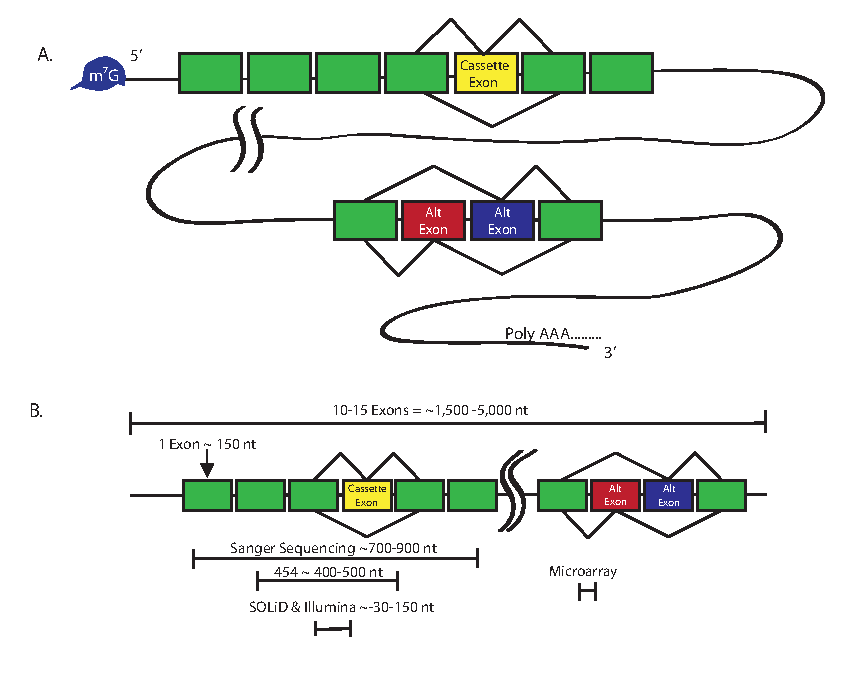
\includegraphics{Figures/Chapter1/SeqLengths_and_Connectivity.pdf}
	\caption[HTS read lengths are not sufficient to maintain AS connectivity]
	{
		HTS read lengths are not sufficient to maintain AS connectivity\\[0.25cm]
		A) Long RNAs may have multiple sites of AS, separated by 1000's of nt; B) Most mRNAs have ~10 exons of ~150 nt each. Some have many more (and longer) exons. Read lengths of current sequencing technologies do not maintain connectivity between distant sites.
	}
	\label{fig:NoConnectivityInHTSMethods}
\end{figure}
%% ############# FIGURE

Microarrays rely on hybridization of a target sequence to a known probe averaging 25 to 100 nt in length \citep{Southern2001}. Therefore, microarrays indicate only the presence of short sequences in the target sample and do not provide adequate linkage information of these sequences. A hypothetical scenario can be used to describe it another way. Say we are investigating a transcript known to display two different regions of AS (See Figure \ref{fig:NoConnectivityInHTSMethods}). Probes targeting these two regions demonstrated an increase in signal for both AS events. Unfortunately, we could not determine if we observed an increase in unique transcripts, each containing only one region of AS, or an increase in production of a single transcript containing both regions \citep{Calarco2007}. This binary analysis is the heart of the "connectivity problem." Microarrays have proven extremely informative and will likely continue to do so in more targeted applications. However, this issue, combined with concerns of cross-hybridization, reproducibility, and a comparably small dynamic range, will likely hasten microarray displacement by RNA-Seq as the preferred method for comprehensive analysis of gene expression \citep{Shendure2008}.

Many researchers are turning toward 2nd generation HTS methodologies for comprehensive transcriptome analysis. This sequencing approach has significance advantages over microarrays. Specifically, it allows de novo identification of isoforms, over a larger dynamic range, in a quantitative fashion \citep{Mortazavi2008}. Additionally, techniques exist to enrich samples for low-abundance isoforms, making the complete cataloging of AS events a possibility \citep{Djebali2008, Salehi-Ashtiani2008}. Unfortunately, the current read-length abilities (depicted in Figure 1-1,B) of all sequencing platforms do not solve the connectivity problem. Excluding single-molecule HTS read lengths of sufficient length \citep{Shendure2004}, other approaches proposed to solve the connectivity problem include traditional cloning and sequencing or hybridization of query oligos to single-molecule transcripts \citep{Zhu2003, Calarco2007, Emerick2007}. While these approaches can determine exon sequence connectivity, they scale poorly and are not feasible for large-scale applications. 
Clearly, AS is an essential regulatory mechanism involved in the control of human gene expression. Its combinatorial nature could potentially answer many questions, such as a physical explanation of what separates us from our closest evolutionary ancestor, the chimpanzee \citep{Calarco2007a}. Additionally, the influence of AS on disease and cancer is slowly coming to light \citep{Tazi2009}. Unfortunately, because of the limitations of methods currently used for the large-scale analysis of isoform expression we fail to obtain the complete picture of AS. One specific missing element of that picture is the prevalence of coordination between different regions of AS separated by large spans of sequence. An efficient, large-scale, single-molecule technique that maintains isoform sequence connectivity is required to complete the complicated picture of AS.

% Need to mention DSCAM – that can be the transition to Coordination in splicing

%----------------------------------------------------------------------------------------
\subsection{Coordination in splicing}
%----------------------------------------------------------------------------------------

% <Consider a leadin with this paper, Osheim YN, Miller OL Jr et al (1985) RNP particles at splice junction sequences on Drosophila chorion transcripts. Cell 43(1): 143–151> That shows spliceosomes associated with nascent RNA transcripts

%< Also consider referencing and discussing the Mediator complex and its effect on downstream splicing - read this paper: Bieberstein NI, Carrillo Oesterreich F, Straube K et al (2012) First exon length controls active chromatin signatures and transcription. Cell Rep 2(1):62–68

Identification of proximally acting SREs is progressing at a rapid pace. New and traditional biochemical methods, coupled with HTS, will undoubtedly fuel this progress. Unfortunately, a critical component of AS regulation currently neglected by the field is that of SREs acting across a considerable distance (>800 nt). One observation that may lead to the identification of long-range SREs is intramolecular coordination between distal splicing decisions. Figure \ref{fig:NoConnectivityInHTSMethods} a model transcript that may exhibit coordinated distal regions of AS. In this model, the 5\textprime~ region of AS contains a cassette exon, which may or may not be included. This region is separated from the 3\textprime~region of AS by many thousands of nucleotides. Does the decision to include the cassette exon have an effect on which of the mutually exclusive exons is included? This type of AS regulation may represent a general and pervasive phenomenon.

%% ############# FIGURE
\begin{figure}[htbp]
	\centering 
	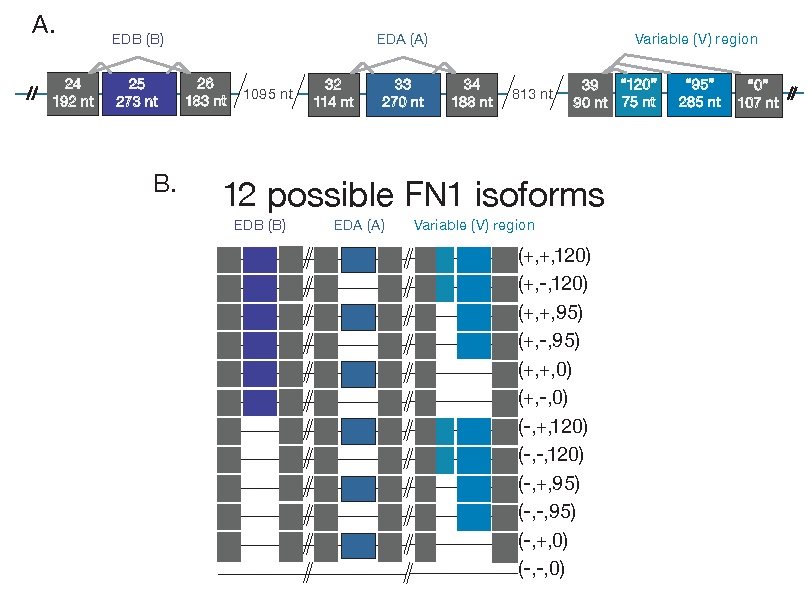
\includegraphics{Figures/Chapter1/Fibronectin.pdf}
	\caption[Mouse \fn{} contains multipe sites of Alternative Splicing]
	{
		Mouse \fn{} contains multiple sites of Alternative Splicing\\[0.25cm]
		A) There are three highly-studied regions of AS in mouse \fn{}: The cassette exons EDB and EDA, and the Variable(V)-region (AKA the IIICS) exon, which displays multiple 3\textprime~ splice sites.  Each of these sites is separated by multiple constitutive exons.; B) Considering simplistic splicing of these three exons, there are 12 different isoforms of mouse \fn{}.
	}
	\label{fig:mouseFn1}
\end{figure}
%% ############# FIGURE

There is precedence in the literature for genes known to display coordinated regions of AS. One of the clearest examples is mouse Fibronectin \fn{} (Figure \ref{fig:mouseFn1}) \citep{Schwarzbauer1983, White2011a}. In this gene, inclusion of the alternatively spliced Extra Domain A (EDI or EDA) region promotes splicing from one of three alternative 3\textprime~ Splice Site (3\textprime~ SS) in the type III homology connecting segment (IIICS) region, resulting in more frequent production of shorter transcripts \citep{Fededa2005}. This effect occurs over six constitutively expressed exons and 800 nt of sequence (5400 nt if introns are considered). \citep{Fededa2005} also analyzed EST databases, concluding that approximately 25\% of human genes contain multiple regions of AS. How many of these regions could show a coordinated effect, similar to that observed in Fibronectin? Providing some insight into this question, Fagnani et al used microarrays designed to report on inclusion levels of cassette exons in mammalian central nervous system tissues \citep{Fagnani2007}. The results produced a set of 38 pairs of exons mapping to the same gene that showed a coordinated increase or decrease of inclusion levels. 

There have been a few studies that investigate forms of splicing coordination between adjacent exons present in mRNA. The vertebrate genes 4.1B and 4.1R, members of the protein 4.1 family encoding for cytoskeletal adaptor proteins, both undergo splicing of upstream 5\textprime~ first exons to distal 3\textprime~ second exons, skipping a stronger proximal 3\textprime~ second exon \citep{Parra2008, Parra2012}. This is accomplished through 'intrasplicing' involving an intronic sequence element (the 'intraexon') only present when transcription begins at the upstream 5\textprime~ exon, allowing the exon to ligate do the weaker distal 3\textprime~ second exon via an intermediate splicing event. Importantly, this type of splicing would be similar, but different from recursive splicing seen in drosophila \citep{Burnette2005}. Another example of the importance of intron sequence elements on AS is observed in the equine $\beta$-casin gene, where the authors propose a model involving an intronic splicing enhancer bound to the exit channel of the elongating polymerase, promoting inclusion of downstream cassette exons \citep{Lenasi2006}. Taking a more genome-wide approach Peng et al. examined human and mouse EST data looking for correlations between adjacent AS cassette exons \citep{Peng2008}. The authors note that positively correlated pairs of adjacent cassette exons typically resemble constitutive exons in splice strength, whereas negatively, or weakly correlated pairs are likely to be newly emerging exons, whose strength of splicing has not evolved enough to be constitutively included. 

The last, most current, and thorough study of intra-gene splicing coordination involves the \textit{Caenorhabditis elegans} gene \slo{} \citep{Glauser2011, Johnson2011}. \slo{} is the \textit{C.elegans} orthologue of the human BK channel gene \kcnma{}, also known to undergo extensive alternative splicing \citep{Nilsen2010} via 13 cassette exons, potentially coding for over 1,000 different isoforms. \kcnma{} is highly developmentally, spatially, and tissue regulated. It is involved in a diverse range of cellular processes, including hearing, circadian rhythms, urinary function, and vasoregulation \citep{Fodor2009a}. While the gene is highly conserved, as organism complexity grows, so does the apparent transcriptional diversity of this gene. In worms, \slo{} can produce up to 12 different isoforms. Glauser et al. used QPCR to demonstrate individual, AS region inclusion frequencies do not correspond to complete isoform frequencies, when measured via a TaqMan probe approach. They go on to describe a interdependent-splicing model that best fits the data, and support interdependence via mutations at one sight altering splicing at both upstream and downstream sites of AS, separated by atleast one other splicing event. After measuring the biophysical properties of the isoforms \citep{Johnson2011}, they conclude that coordinated AS is critical for proper BK channel function in vivo. It is interesting to note that this study also identified an intronic sequence element that displayed some type of coordinated, or co-regulated effect on AS. 

%Optional continue on with discussion and include Discuss long range RNA secondary structure and implecations of regulating alternative splicing (See Li, S., & Breaker, R. R. (2013). Eukaryotic TPP riboswitch regulation of alternative splicing involving long-distance base pairing. Nucleic acids research, 41(5), 3022–31. doi:10.1093/nar/gkt057) and Reg of AS by long RANGE SS folder in Mendeley


%----------------------------------------------------------------------------------------
\subsection{Many isoforms per gene}\label{sec:IsoformsPerGene}
%----------------------------------------------------------------------------------------

It is easy to think of AS as a binary process. Isoform A or B is produced based upon picking either exon A or B. What quickly becomes evident, and is far too real for researchers building transcriptome assembly algorithms, is that the combinatorial nature of AS makes it both a power means of generating isoform diversity and a difficult problem to study \citep{Trapnell2012a}.
 
%% ############# FIGURE
\begin{figure}[htbp]
	\centering 
	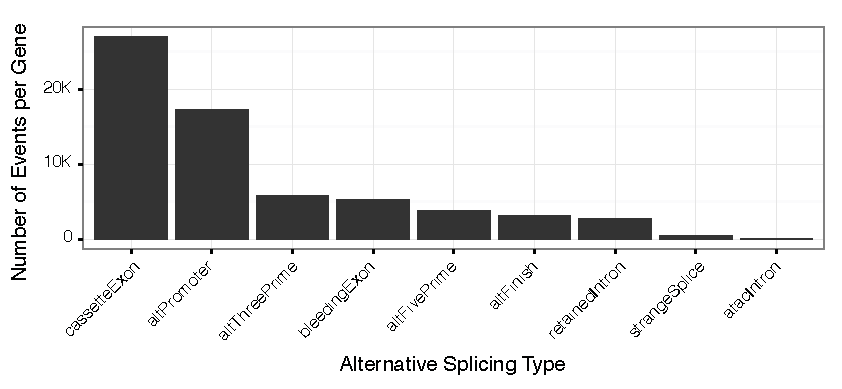
\includegraphics{Figures/Chapter1/ASEventTypesPlot.pdf}
	\caption[Number of hg19 Alternative Event types per gene]
	{
		Number of hg19 Alternative Event types per gene\\[0.25cm]
		Alternative Event types per gene. RefSeq on 2014-03-24
	}
	\label{fig:asEventsBarChart}
\end{figure}
%% ############# FIGURE

One of the most recent attempts to investigate the breath of combinations produced by AS is the already mentioned ENCODE project \citep{Djebali2012}. ENCODE performed extremely in depth analysis of 15 cell lines, and find that each isoform produces ~10 transcripts per gene, with a broad distribution in terms of isoforms expressed per sample. 

The ENCODE project clearly demonstrated that most human genes can under AS in many more ways than previously appreciated. Most genes could be considered as undergoing 'complex' AS, with numerous forms of AS ( See figure \ref{fig:asEventsBarChart}). Despite the prevalence of complex alternative spliced genes, just a few genes are used as examples to illustrate numerical possibilities and biological significance. For example the human immune system relies heavily on AS to be plastic toward antigen recognition and response \citep{Lynch2004}. Modulation of extracellular signaling proteins such as \textit{CD44} and cellular adhesion protein \textit{CD45} have been well-studied \citep{Zikherman2008,Ponta2003b}. Alternative splicing in humans, however, does not seem to produce the number of unique possible combinations as AS of genes in simpler organisms, such as fruit flies, perhaps due to specialization of genes, or different genes that work in combination or complexes, as oppose to utilizing unique gene isoforms \citep{Park2007}. For example, the fruit fly gene muscle myosin heavy chain (\textit{Mhc}) can produce up to 480 different isoforms through AS of 17 different cassette exons \citep{Bernstein1983a}.  

%% ############# FIGURE
\begin{figure}[htbp]
	\centering 
	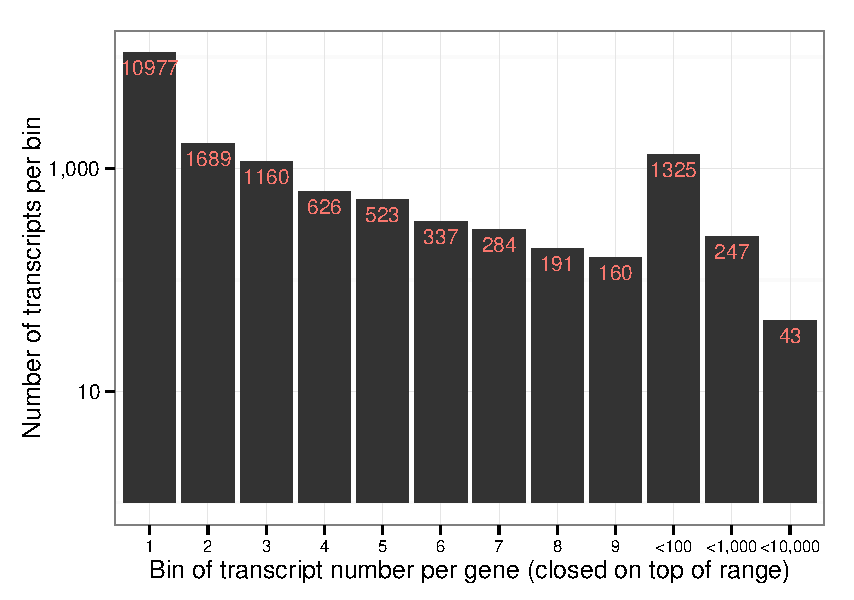
\includegraphics{Figures/Chapter1/NumberOFTranscriptsPerFlyGene.pdf}
	\caption[Number of transcripts per \flies{} gene]
	{
		Number of transcripts per \flies{} gene\\[0.25cm]
		Data from \citep{Brown2014}, Supplemental Table 3. Number of transcript per bin, with bin sizes 'closed' on the upper part of range.
	}
	\label{fig:txPerFlyGene}
\end{figure}
%% ############# FIGURE

%% ############# Table
\renewcommand{\arraystretch}{0.5}
\small
\begin{tabular}[c]{l|r|r|r}
	\hline
	\textbf{Gene Name} & \textbf{\# Introns} & \textbf{\# Transcripts} & \textbf{\# Proteins}\\
	\hline
	Mhc & 60 &  2040 & 511\\
	\hline
	slo & 49 &  2070 & 279\\
	\hline
	ps & 30 &  2099 &  27\\
	\hline
	rg & 45 &  2178 &  23\\
	\hline
	shot & 60 &  2478 & 886\\
	\hline
	scrib & 53 &  2555 & 259\\
	\hline
	heph & 75 &  2876 &  52\\
	\hline
	CG42748 & 26 &  2876 &  51\\
	\hline
	rdgA & 35 &  3003 &  89\\
	\hline
	Mbs & 39 &  3080 & 119\\
	\hline
	CaMKI & 41 &  3992 &   7\\
	\hline
	par-1 & 48 &  4410 & 142\\
	\hline
	GluClalpha & 27 &  4945 & 188\\
	\hline
	Sap47 & 24 &  5011 &  49\\
	\hline
	Patronin & 50 &  5615 & 590\\
	\hline
	CG17838 & 37 &  8333 & 147\\
	\hline
	unc-13 & 52 &  8391 & 279\\
	\hline
	A2bp1 & 29 &  9055 &  58\\
	\hline
	Imp & 33 &  9131 &  12\\
	\hline
	pan & 38 &  9432 &  72\\
	\hline
	Sh & 40 & 15995 &  66\\
	\hline
	gish & 48 & 18972 & 142\\
	\hline
  \end{tabular}
%% ############# Table

%----------------------------------------------------------------------------------------
\subsection{\flies{} \dscam{}}\label{sec:Dscam}
%----------------------------------------------------------------------------------------

Unquestionably, the gene most frequently used to demonstrate the combinatorial power of AS is fly \dscam{}. The 'architecture' of \dscam{} is rather unique among other organisms, but as we saw in Section \ref{sec:IsoformsPerGene}, contain some genes that generate tremendous isoform diversity from a single genetic locus \citep{Brown2014}. The basic structure of \dscam{} is shown in Figure \ref{fig:DscamArch}.

%% ############# FIGURE
\begin{figure}[htbp]
	\centering 
	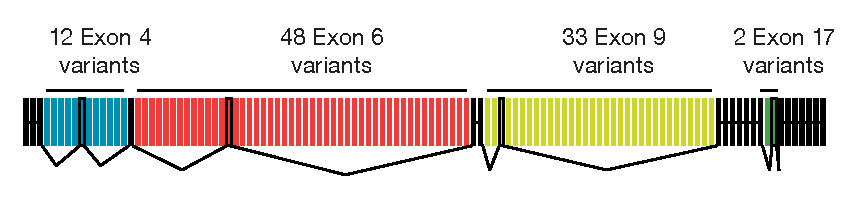
\includegraphics{Figures/Chapter1/DscamArch.pdf}
	\caption[The architecture of the \flies{} gene \dscam{}]
	{
		The architecture of the \flies{} gene \dscam{}\\[0.25cm]
		\dscam{} has three \textit{clusters} or 'banks' of alternative cassette exons that are splicing out in a mutually-exclusive manner. The first bank, 'Exon 4', contains 12 different variants, of which one one is ever included into the mRNA. Similarly, banks 6 \& 9 each contain 48 and 33 different variants, respectively. These three banks code for extracellular IgG domains, while the final region of AS, exon 17, encodes two different trans-membrane domains, again of which only one is included in the final mRNA.
	}
	\label{fig:DscamArch}
\end{figure}
%% ############# FIGURE

Human \textit{Dscam}, for which \dscam{} was named, was identified while looking for genes on chromosome 21, specifically band 21q22, where extra copies expressed in Down syndrome patients, a trisomy 21 disorder, may be causative for disease \citep{Yamakawa1998b}. \textit{Dscam} (Down Syndrome Cellular Adhesion Molecule) was named according to this association, and its membership in the immunoglobulin super family of proteins with extracellular adhesion functions. Human \textit{Dscam} does undergo some alternatively splicing and broadly expressed in the developing nervous system. However, it does not contain the architecture of cassette exon banks as \dscam{}.

Complex AS of\dscam{} was first noticed by the Zipursky lab in 2000 \citep{Schmucker2000}. While looking for proteins associated with \textit{dock} and \textit{pak}, two proteins important for neuronal growth cone guidance, they biochemically co-purified DSCAM1. Sequencing of \dscam{} clones revealed that virtually all contained different combinations of exons 4,6, and 9. In fact, these three exons are chosen from three clusters of mutually-exclusive cassette exons, containing 12, 48, and 33 different options each(see Figure \ref{fig:DscamArch}). The initial report kicked off an exciting period of research into \dscam{} structure and function. The functional significance of \dscam{} AS was a major goal of multiple labs.

Before the highlights of \dscam{} research are reviewed, it is illustrative to discuss some basic \flies{} anatomy. There are 4 main regions where \dscam{} expression has been highly-studied.

\begin{itemize} \itemsep0.5pt \parskip0pt \parsep0pt
  \item Hemocyte cells of the immune system
  \item Larva Class IV da Neurons 
  \item Pupal Mushroom-body neurons in the developing brain
  \item Tetrad synapses of the eye
\end{itemize}

\dscam{} involvement/expression in three of these four  biologically important roles is shown in Figure \ref{fig:DscamAnatomy}. First, \dscam{} expression in hemocyte cells of the immune system is important for recognition of foreign antigens \citep{Watson2005}. During larval development, \dscam{} is expressed in the da neurons of the larval body wall, these neurons create a uniform sensory feed, allowing the larva to respond to mechanical stimulus. In the developing brain, \dscam{} is expressed in both axonal projections of neurons extend from their Kenyon cell bodies and bifurcate into two different mushroom body lobs \citep{Zhan2004}. 

%% ############# FIGURE
\begin{figure}[htbp]
	\centering 
	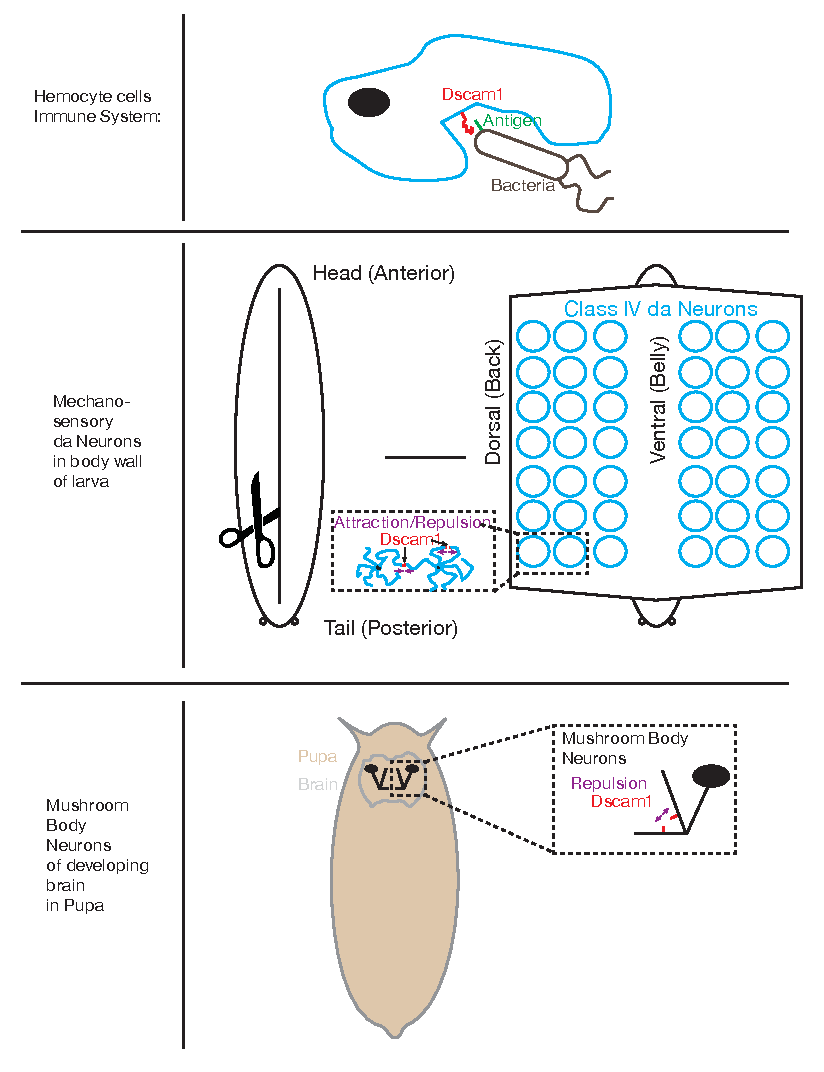
\includegraphics{Figures/Chapter1/DscamAnatomy.pdf}
	\caption[Important \dscam{} expression during \flies{} life cycle]
	{
		Important \dscam{} expression during \textit{Drosophila melanogaster life} cycle\\[0.25cm]
		\dscam{} has been high-studied in four different regions/cell types. 1) Hemocytes of the immune system, where DSCAM1 is involved in antigen recognition; 2) In Class IV da neurons, which sense mechanical stimulation of the larval body wall; 3) In mushroom body neurons of the pupal developing brain; and 4) (not shown) in Tetrad neurons of the eyes.
	}
	\label{fig:DscamAnatomy}
\end{figure}
%% ############# FIGURE


%Papers to discuss.
	%2. Graveley 2001 - Regulation \citep{Graveley2001}
	%3. Umass guy Suman lee = Not sure 
	%4. Neves 2004 - Diversity \citep{Neves2004a}
	%5. Zhang 2004 - Diveristy \citep{Zhan2004}
	%6. Graveley 2004 – Selector and Docking \citep{Graveley2004}
	%7. Schmucker science 2005 – Diversity, Immunity \citep{Watson2005}
	%8. Hattori series – Minimal require divsersity \citep{Hattori2005a,Hattori2008,Hattori2009}
	%9. The cell paper mattori 2013 – Diversity dynamics, bunch of other cool stuff. \citep{Miura2013b}

% Need transition from Dscam to Rnl2!

%----------------------------------------------------------------------------------------
\section{Nucleic Acid Ligation}
%----------------------------------------------------------------------------------------
\subsection{RNA Sequence investigation by ligation}\label{sec:Ligation}
%----------------------------------------------------------------------------------------

In the late 1960's and early 1970's, the Lehman and Richardson labs characterized two workhorse-enzymes of modern molecular biology. Robert Lehman and colleagues, working at Standford Medical School, first described the activity of \textit{polynucleotide-joining enzyme} from \textit{Escherichia coli} (now known as \textit{E. Coli} DNA Ligase) \citep{Olivera1967b}. Work on this enzyme paralleled that from the Richardson lab at Harvard Medical School, where they focused on \textit{polynucleotide ligase} from \textit{Escherichia coli} infected with T4 bacteriophage (now known as T4 DNA ligase) \citep{Weiss1967a}. It became clear that while these two enzyme's shared a common mechanism\textemdash later elucidated by \citep{Modrich1973a}\textemdash they had important differences. First, T4 DNA ligase required ATP as a cofactor, which \textit{E. Coli} DNA Ligase did not (though it was later discovered that DNA ligase required NAD as a cofactor). Second, only T4 DNA ligase could catalyze ligation of blunt-ended DNA \citep{Tabor1987a}.

%% ############# FIGURE
\begin{figure}[htbp]
	\centering 
	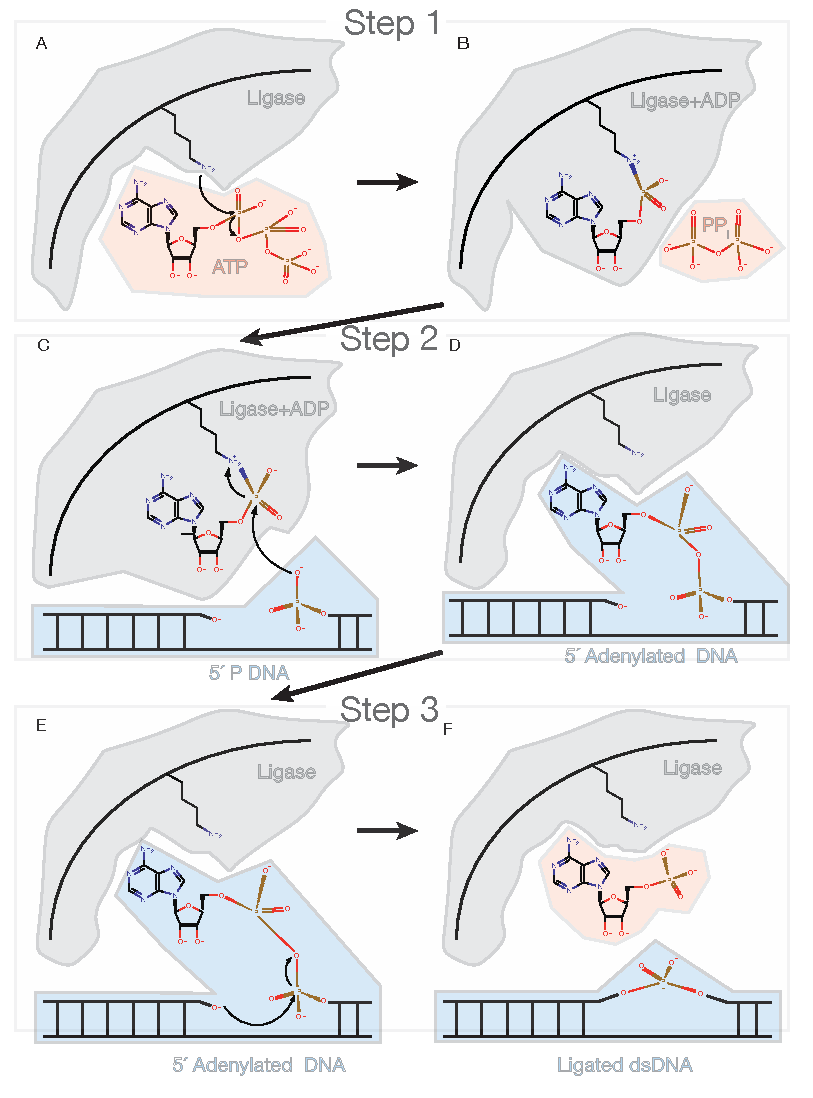
\includegraphics{Figures/Chapter1/LigationMechanism.pdf}
	\caption[Mechanism of Rnl2 ATP-dependent ligation]
	{
		Mechanism of ATP-dependent ligation\\[0.25cm]
		Adapted from \citep{Nandakumar2006} and specifically for that of T4 RNA ligase 2.
	}
	\label{fig:Ligation Mechanism}
\end{figure}
%% ############# FIGURE

The general mechanism of ligation, shown in Figure \ref{fig:Ligation Mechanism}, involves three steps: Step 1 (A) involves the $\epsilon$-amino group from the active site lysine performs a nucleophilic attack on the $\alpha$-phosphate of ATP in solution.  B) The ligase is now charged with AMP and inorganic phosphate (PPi) is freed into solution. C) Step 2: Nucleophilic attack by the 5\textprime~ DNA phosphate on the 3\textprime~ side of the nick to the AMP:ligase phosphate. D) 'Adenylated' DNA is now competent for DNA ligation. E) Step 3: the 3\textprime~ OH on the 5\textprime~ side of the nick performs a nucleophilic attack on the 5\textprime~ PO$_{4}$ across the DNA nick, liberating AMP into solution. F) Sealed nick resulting in: Ligase; AMP; and intact dsDNA.

In addition to elucidated the general mechanism of ligation, it was also discovered that T4 DNA ligase lacks a preference for terminal polynucleotide structures. The Khorana and Richardson labs both reported the activity of this enzyme on combinations of RNA and DNA duplexes \citep{Fareed1971, Kleppe1970b}. Both of these papers describe an activity on T4 DNA ligase, \underline{RNA-templated DNA to DNA ligation}, that is of particular relevance to this thesis work. Unlike T4 DNA ligase, \textit{E. Coli} DNA Ligase, will not join DNA strands on an RNA template \citep{Bullard2006}. Soon after demonstrating these activities in vitro, the Khorana lab reported detection of organism-generated DNA \citep{Besmer1972b}, setting up an orthogonal field (respective to PCR) of nucleic acid sequence characterization \citep{Conze2009c}.

An enzyme that can catalyze an RNA-templated DNA:DNA ligation is a very useful molecular biology tool for two main reasons. First, using RNA as a ligation guide means no modification is made to the template molecule. This contrasts cDNA analysis, where the RNA has been enzymatically converted by reverse transcription, potentially losing valuable RNA-coded information, such as modified bases. Second, synthesis of the DNA probes used in ligation is inherently easier and cheaper compared to synthesis of RNA probes. In addition to being cheaper, synthesis of DNA probes has become high-throughput since the adoption of microarrays as a standard gene expression measurement tool \citep{Schena1995a}. A pair of papers from the Landegren lab first reported the utility of RNA-templated DNA:DNA ligation for analysis of RNA transcripts \citep{Nilsson2000,Nilsson2001}. The Fu lab applied this approach in a multiplex experimental design in collaboration with Illumina \citep{Li2012c,Yeakley2002}, while Mats Nilsson and Ulf Landegren developed a single molecule application \citep{Conze2010}. It is important to note that \textit{all} of these studies used T4 DNA ligase. Clearly, there is interest and utility in analyzing RNA in both high-throughput and multiplex experimental designs, using cheap DNA probes, and without cDNA conversion.

For more than 40 years after its first description, T4 DNA ligase was the only choice for RNA-templated DNA:DNA ligation. However, a recent publication from New England Biolabs (NEB) describes this activity by another well-studied ligase, Chlorella Virus PBCV-1 DNA ligase (herein Chlorella DNA ligase) \citep{Lohman2013d}. Chlorella DNA ligase is a long-studied enzyme and had been reported to \textit{not} display RNA-templated DNA:DNA ligation activity \citep{Ho1997b,Sriskanda1998c}. However, at high enough concentrations and under special buffer conditions (specifically a critical concentration of ATP), Lohman et al have shown that Chlorella DNA ligase will join two DNA strands hybridized to an RNA template \citep{Lohman2013d}. They further demonstrated that it performs no worse in this activity than traditional T4 DNA ligase \citep{Nilsson2001,Yeakley2002}.

Building on the list of available enzymes that join hybrid polymer substrates Chapter \ref{Chapter2} presents data supporting RNA-templated DNA:DNA ligation activity for another enzyme, T4 RNA Ligase 2.

%----------------------------------------------------------------------------------------
\subsection{T4 RNA Ligase 2 (Rnl2)}
%----------------------------------------------------------------------------------------

Proteins of the T4 and T7 bacteriophages have been a boon for molecular biology. Without enzymes like polynucleotide kinase \citep{Richardson1965a}, T7 RNA polymerase \citep{Summers1970b}, and T4 DNA ligase \citep{Weiss1967a}, many essential manipulations of nucleic acids would have been impossible for decades. Obviously, these enzymes also have essential phage functions. T7 RNA polymerase is responsible for late stage replication of T7 phage transcripts, while T4 PNK works in concert with T4 DNA and RNA ligases to repair cleaved	nucleic acids resulting from bacterial pathogens defense systems \citep{Wang2002b}. Specifically, T4 RNA ligase 1 (herein "Rnl1", also known as \textit{gene 63} maintains phage replication by repairing tRNAs cleaved by an anticodon nuclease produces from the \textit{prr} locus \citep{Amitsur1987d}.

Given the utility and importance of these enzymes, novel enzyme discovery is a fruitful area of research. The Shuman lab has a distinguished record of discovering and characterizing numerous such enzymes, including any involved in nucleic acid synthesis, modification, and repair. Through a blast search looking for novel ligases with sequences related to \textit{Trypanosoma brucei} RNA-editing ligases TbMP52 and TbMP48 \citep{Ho2002b}, they identified motifs in correct arrangement, spacing, and number indicative of an RNA ligase. The gene, identified as \textit{gp24.1}, has quickly become an essential tool in the era of modern genomics.

Initial biochemical purification and characterization of \textit{gp24.1} \citep{Ho2002b} revealed that it indeed codes for an RNA ligase, which was renamed T4 RNA ligase 2 (herein "Rnl2"). Rnl2 is a 374 amino acid monomeric protein composed of 2 distinct domains initially purified as a 42-kDA His-tagged recombinant protein. The N-terminal domain (1\textendash 243) is responsible for steps (1) and (3) of the general ligation mechanisms (see Figure \ref{fig:Ligation Mechanism}), while the C-terminal domain (244\textendash 329) is responsible for adenylation of the 5\textprime~ PO$_{4}$ on the 5\textprime~ residue at the 3\textprime~ side of the nick, as shown in step (2). Additionally, Rnl2 is routinely purified as a pre-adenylated and immediately poised for its first ligation. In contrast to the N-terminal domain, which is composed of motifs typical to main ligases, the C-terminal domain is significantly	different from all other DNA ligases and has no structural homologue. While the biological function of Rnl1 is known, the biological function of Rnl2 remains a mystery, more than 12 years after its discovery \citep{Chauleau2013b}. However, there is some speculation that the flurry of research into bacterial CRISPR phage defense may reveal a role for Rnl2 \citep{Barrangou2007c,Chauleau2013b}.

%% ############# FIGURE
\begin{figure}[htbp]
	\centering 
	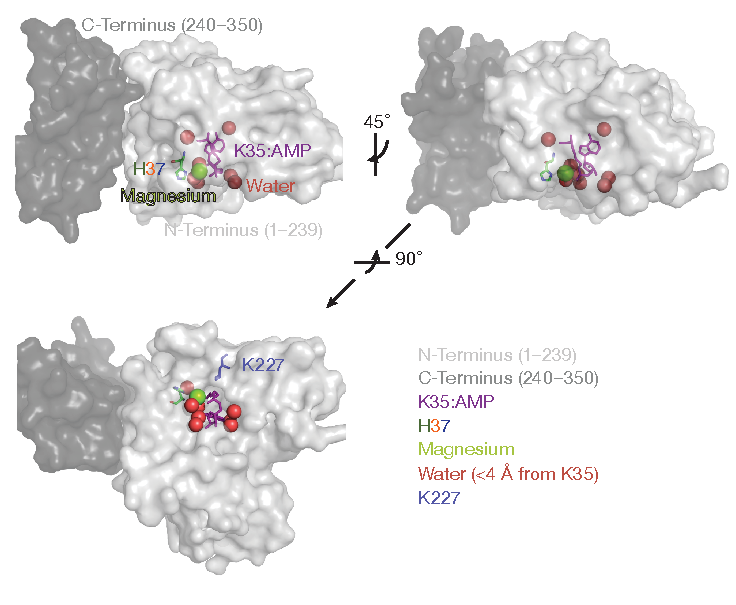
\includegraphics{Figures/Chapter1/Rnl2_Structure.pdf}
	\caption[Structure and active site of pre-adenylated of Rnl2]
	{
		Structure and active site of pre-adenylated of Rnl2\\[0.25cm]
		Rnl2 as crystalized and described by \citep{Nandakumar2006}. Structures from PDB:2HVQ were generated with PyMol. Top left) Rnl2 is composed of a C-terminal and N-terminal domain. Top Right) The active site of Rnl2 is highlighted. Bottom left) Active site of Rnl2 as shown from bottom. This face interacts with substrate. Residue numbering refers to that of the crystal structure.
	}
	\label{fig:Rnl2 General Structure}
\end{figure}
%% ############# FIGURE

Mutational analysis of Rnl2, and later a crystal structure of the enzyme, have identified key functional residues \citep{Ho2004, Nandakumar2006,Nandakumar2004a,Yin2003d}. The lysine residue at position 35 (K35) receives the AMP in Step 1. The K227 residue in the C-terminal domain is essential for both forward and reverse adenylation of the 5\textprime~ PO$_4$ at the nick \citep{Viollet2011}. Mutation of H37 results in an ~102 reduced ligation rate, and therefore indicates the essential nature of this residue. Finally, T39 has been shown to interact with the 2\textprime~ OH on the 3\textprime~ side of the nick, preferring a C3\textprime~ endo sugar pucker confirmation (see Figure \ref{fig:Rnl2 Active Site Residues}). Rnl2 has a minimal footprint of 13nt, centered on the nick, and only requires magnesium for transfer of AMP to the 5\textprime~ phosphate. Work done in the Shuman lab \citep{Nandrakumar2006} observed that 2\textprime~ deoxyribose residues on the 5\textprime~ side of the nick (i.e. DNA) adopt an RNA-like sugar pucker, leading to the correct orientation of the 3\textprime~ OH relative to the AMP leaving group and resulting in ligation. This conformation is of particular importance to this results presented in Chapter \ref{Chapter2}.

%% ############# FIGURE
\begin{figure}[htbp]
	\centering 
	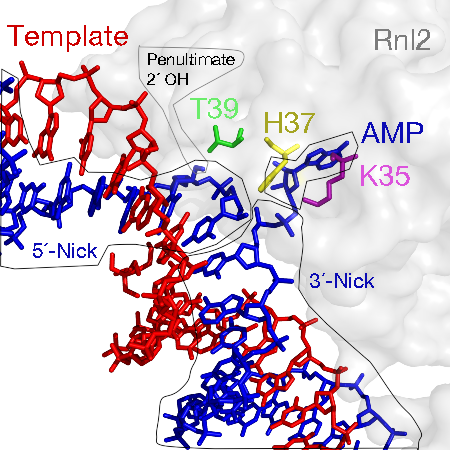
\includegraphics{Figures/Chapter1/Rnl2_Active_Site_Residues.pdf}
	\caption[Active site of T4 RNA Ligase 2 with highlighted residues]
	{
		Structure and active site of pre-adenylated of Rnl2\\[0.25cm]
		Rnl2 complexed with nicked dsDNA as crystalized and described by \citep{Nandakumar2006}. Structures from PDB:2HVR and generated with PyMol
	}
	\label{fig:Rnl2 Active Site Residues}
\end{figure}
%% ############# FIGURE

While Rnl2 is extremely efficient at high concentration, displaying little or no reversible chemistry, a modified version of the enzyme containing only the N-terminal domain and a K227A point mutation (“Truncated mutant”) has no adenyltransferase activity. In this case, adenyltransferase refers to the ligase transferring AMP from an adenylated substrate to itself; reverse chemistry of step 2 in Figure \ref{fig:Ligation Mechanism}). This mutant has been used in specialized cloning applications \citep{Ghildiyal2008, Hafner2008a, Viollet2011} that take advantage of this activity. In these reactions, the use of pre-adenylated 3\textprime~ DNA adaptors allows for selective ligation among already phosphorylated species by limiting the enzyme-catalyzed transfer of AMP from the adaptor to other phosphorylated species. Use of this truncated mutant to create a hybrid RNA/DNA molecule has greatly improved many high-throughput sequencing work flows.

Ligation of hybrid substrates (eg. DNA-templated RNA:DNA vs DNA-templated DNA:DNA) have revealed general substrate preferences. DNA ligases appear to prefer the residue bearing the 5\textprime~ phosphate on the 3\textprime~ side of the nick to be 2\textprime~ deoxyribose, and have a relaxed requirement for the sugar on the 5\textprime~ side of the nick. RNA ligases have the reverse preference, demonstrating higher activities when the 5\textprime~ strand, 3\textprime~ OH residue also bears a 2\textprime OH. Rnl2 has an additional preference for an RNA residue at the penultimate 3\textprime~ side of a nick \citep{Ho2002b,Ho2004, Nandakumar2004a, Nandrakumar2006}. The two base requirement for RNA at the 5\textprime~ side of the double stranded nick biases Rnl2 to join RNA:[RNA/DNA] strands. Independent labs have measured this preference and have reported that the RNA-templated DNA:DNA joining activity of Rnl2 is below assay limits of detection \citep{Bullard2006}. However, results discussed in this work clearly show that with enough enzyme, and sensitive downstream measurements, Rnl2 will catalyze RNA-templated DNA:DNA ligation (see Chapter \ref{Chapter2}. Previous reports of Rnl2 lacking this activity are likely due to a single turnover mechanism in this reaction, owning to the poor dissociation rate of nucleic acid-interacting enzymes.
 % Need to add reference to this paper - \cite{Reuveni2014} where they talk about the importance of enzyme unbinding to the speed of reactions. That doesn't get at a reference that talks about slow dissociation of nucleic-acid interacting proteins, for which even Wee said he didn't know a fantastic reference.

% Transition from Rnl2 to long RNAs/ piRNA precusors somehwow. 

 %----------------------------------------------------------------------------------------
 \section{Long Nucleic Acid Polymers}\label{piRNA section}
 %----------------------------------------------------------------------------------------
 %----------------------------------------------------------------------------------------
\subsection{Mouse piRNAs are different}\label{sec:Mouse piRNAs}
%----------------------------------------------------------------------------------------

% ! Incorporate salient points of the Resources paper into this section? At least the sections I worked on!
% Notes from Wei's Group meeting update on piRNAs.
% Mention the Saito 2006 Slicer activity, in vitro, of Piwi domain containing argonautes in flies. Then mention papers from Siomi and Brennecki, and Lin lab in 2009 about mutating the catalytic triad in the piwi proteins and there is no slicer activity. 
% A regulatory circuit for Piwi by the large…
% Transcriptional Silencing of Transposons
% Function of piwi(?) - Lin lab paper.
% Mention review in G&D by hannon title is state of piRNA in flies - says that the slicer activity of piwi proteins in flies has never been shown in vivo. 
% Mention Siomi Zuchi paper - they show in vitro evidence that the protein can take a 5' phosphate ssRNA and make something - a piRNA?

Mammalian spermatogenesis is critical for the future of the species. Recently the importance a specific kind of small RNA\textemdash piRNAs\textemdash for proper spermatogenesis has become clear \citep{Siomi2011}. Even after >12 years since their discovery in \flies \citep{Aravin2001}, and >6 since their identification in rodents \citep{Girard2006, Lau2006}, the essential mechanisms of piRNA biogenesis to proper mammalian spermatogenesis remains largely unknown. These unknown mechanisms include: biogenesis from transcript to small RNA, physiological targets, and terminal function of sterility maintenance. What is known is that without a functioning piRNA pathway males are sterile. Studies in humans have also linked SNPs in the Argonaute proteins that bind piRNAs to decreased fertility \citep{Gu2010a}. 

 %% ############# FIGURE
\begin{figure}[htbp]
	\centering 
	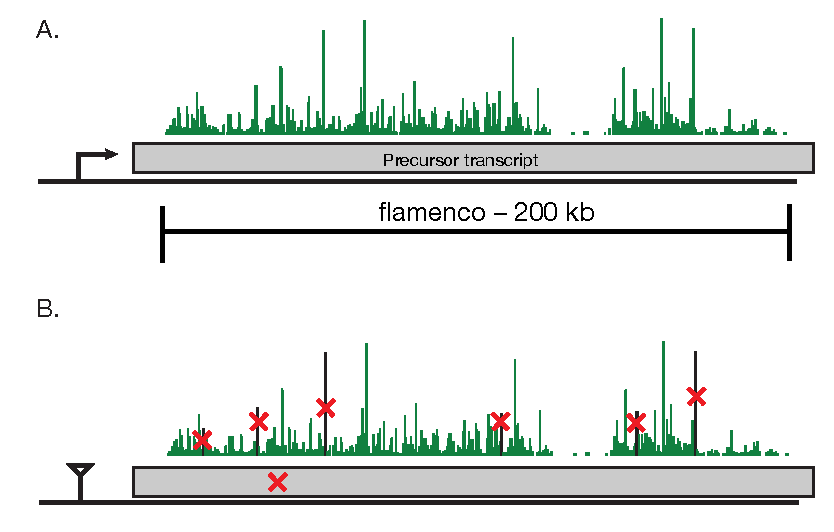
\includegraphics{Figures/Chapter1/FlamencoLocus.pdf}
	\caption[Genetic evidence for long, continuous fly piRNA precursor transcripts]
	{
		A the \flies{} gene \textit{flamenco} is a graveyard for transposon sequences \citep{Pelisson1994}. Evidence for expression of a single-contiguous RNA transcript from \textit{flamenco} (A) is provided by a P-element insertion into the suspected promoter region (B). \citep{Brennecke2007} could not detect specific piRNAs (red X's) by northern blot in the P-element mutant.
	}
	\label{fig:flamenco}
\end{figure}
%% ############# FIGURE


piRNAs are so-called because they bind PIWI proteins, a sub-group of the Argonaute protein family, whose other members utilize small RNA as guides to target nucleic acids for many forms of post-transcriptional regulation \citep{Siomi2011}. There are three PIWI proteins in mice, each displaying a distinct expression profile during development and an association with piRNAs of a specific length. The first PIWI protein expressed, even before a mouse is born, is MIWI2 \citep{Carmell2007}, followed quickly by the more consistent player, MILI (see Figure \ref{fig:mouse piRNA over time} \citep{Kuramochi-Miyagawa2004, Aravin2006}. It is during the 'fetal' stage of piRNA biogenesis in mice that MIWI2 and MILI undergo ping-pong amplification, similar to that observed in flies, in order to silence expression of transposons during germ line formation \citep{Brennecke2007, Kuramochi-Miyagawa2008}. After birth, and during the 'neonatal stage' only MILI is expressed, and piRNAs shift from mostly transposon-mapping to 3\textprime~ UTR mapping \citep{Robine2009}. Once the 'first wave' of spermatogenesis \citep{Oakberg1956b, Laiho2013a} reaches meiosis, the pachytene piRNAs are expressed \citep{Girard2006, Lau2006, Li2013h}. Pachytene piRNAs tend to map to intergenic 'clusters' of unique genomic sequence. These clusters, from here after called 'piRNA-generating genes' appear to produce a single, continuous, relatively long, and un-spliced Pol II transcript \citep{Li2013h}. This is comparable to piRNA clusters in flies, such as flamenco, whose transcription can be abolished with a P-element insertion into a putative promoter, as measured by northern blot looking for piRNAs generated 168 kb downstream (see Figure \ref{fig:flamenco} \citep{Brennecke2007}. 
 
 %% ############# FIGURE
\begin{figure}[htbp]
	\centering 
	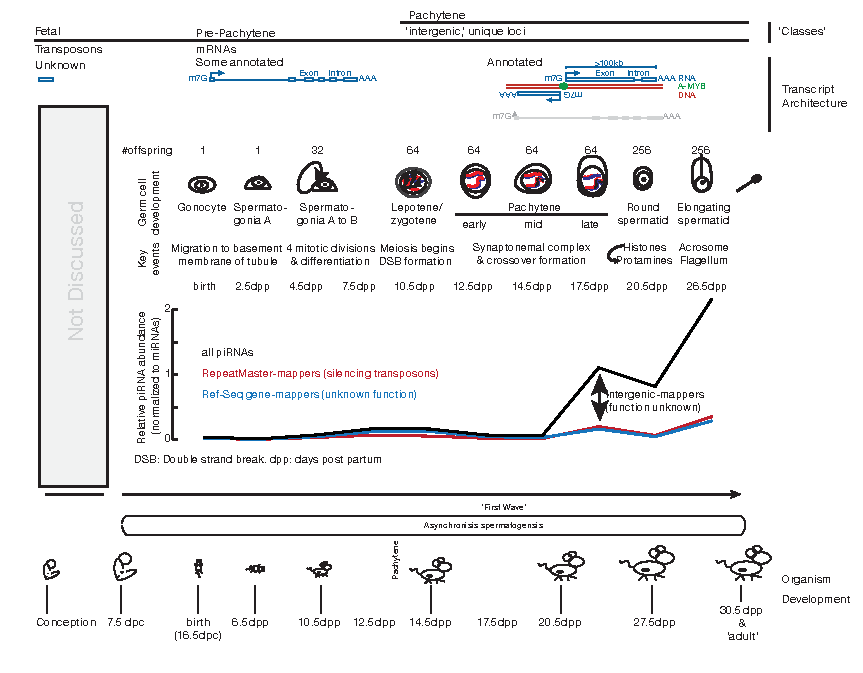
\includegraphics{Figures/Chapter1/MammalianPiRNAClassesOverTime.pdf}
	\caption[Different Classes of mammalian piRNAs]
	{
		\hl{Write a nice caption here!}
	}
	\label{fig:Mammalian piRNA classes}
\end{figure}
%% ############# FIGURE

Mammalian piRNAs can be divided into three major classes (\#Figure of my own design on piRNAs) \citep{Kuramochi-Miyagawa2008}. The first, present before birth, are those of the \textit{fetal piRNAs}. These piRNAs tend to be short, bind the PIWI protein MILI2 in mice, and have sequences found in transposable elements (Carmell et al. 2007). The next class of piRNAs, historically but confusing grouped with the previous class, are called Pre-pachytene piRNAs. Pre-pachytene piRNAs are expressed just before birth, and continue to be expressed in functioning testes, often associated with spermotoXX and spermotXX, precursor cells to mature sperm(?), and tend to map to traditional, and annotated, protein coding genes. Finally, due to their unique sequence in the genome, the genetic origin of a millions of piRNAs belonging to the third class, the pachytene piRNAs, was immediately known. Pachytene piRNAs are extremely abundant after, not coincidently, the pachytene stage of meiosis I when (descriptor) chromosomes pair up, cross over, and rearrange their genetic material. Extremely abundant means XX fold enrichment of pachytene piRNAs compared to miRNAs, as compared to developmental time point just two days earlier. The genomic origins of these piRNAs, while unique in terms of sequence, are often in ‘gene deserts,’ unannotated, and devoid of intronic sequences. This gene architecture makes the pachytene piRNA loci some of the most interesting RNA-producing regions of the mammalian genome.
 
  %% ############# FIGURE
\begin{figure}[htbp]
	\centering 
	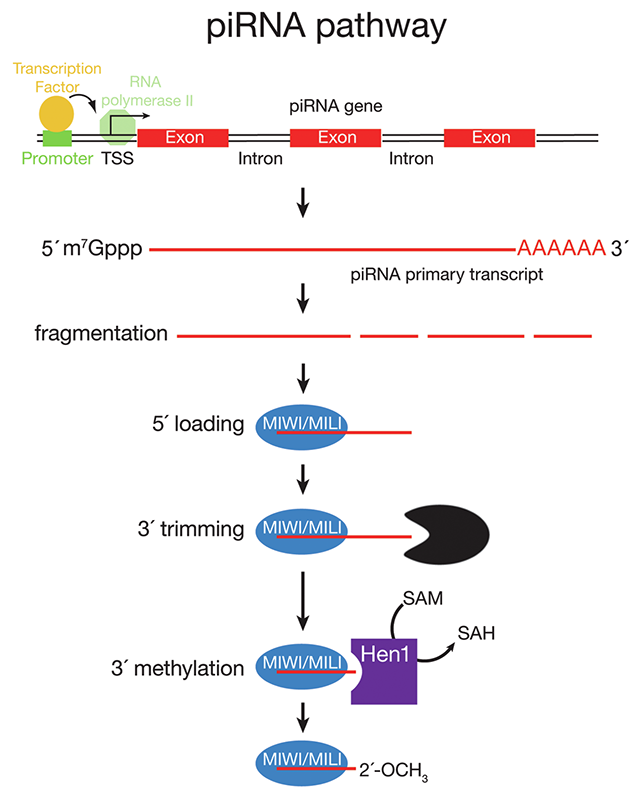
\includegraphics{Figures/Chapter1/mammalian_piRNA_pathway.png}
	\caption[A model for Mammalian piRNA biogenesis]
	{
		Figure taken from \citep{Li2013e}: A model for piRNA biogenesis. Primary piRNA transcripts are transcribed by RNA polymerase II and contain 5\textprime~ caps, exons and introns and poly(A) tails. The transcription of pachytene piRNA genes is controlled by A-MYB; transcription factor(s) (TF) controlling pre-pachytene piRNA genes remain to be discovered. Current models of piRNA biogenesis propose that PLD6 determines the 5\textprime~ end of piRNA intermediates with lengths >30 nt. These intermediates are proposed to then be loaded into PIWI proteins. After PIWI binding, a nuclease is thought to trim the 3\textprime~ end of the piRNA to the length characteristic of the particular bound PIWI protein. Finally, further trimming is prevented by addition of a 2\textprime~-O-methyl group to the 3\textprime~ end of the mature piRNA by the S-adenosylmethionine-dependent methyltransferase HEN1
	}
	\label{fig:Mammalian piRNA BioGensis; MolCel2013 Review}
\end{figure}
%% ############# FIGURE

%!Known functions of mammalian piRNAs
\citet{Vourekas2012} demonstrated that many MIWI, as measured by ClIP, actually bind mRNAs directly, without a small RNA guide.

Two studies \citep{DeFazio2011,Reuter2011} used point mutations in the catalytic triad of MIWI2, MILI to remove slicer activity. The MIWI2 and MILI studies found that the mice were sterile, and did not accumulate transposon-mapping piRNAs. \citet{DeFazio2011} found that the mice were also sterile, and demonstrated increased LINE1 transcript accumulation.  \citet{Reuter2011} states that much the biological activity of MIWI depends on its slicer activity.

%! Comparisons between fly and mammalian piRNA systems
The transposon-mapping nature of the fetal piRNA class made obvious comparisons to the fly piRNA system nature. In the fly system, primary piRNAs transcribed from discrete loci and fed into an amplification loop between two PIWI proteins PIWI(3) and AGO3 (‘the ping-pong’ cycle) (REF Brenneki cell paper 2007). It is believed that PIWI proteins loaded with piRNAs bind and silence transposon messages, using the cleaved transposon transcripts, in combination with primary piRNA transcripts, as a substrates in the Ping-Pong cycle %($REF some newer review demonstrating this activity). 

%! Our annotation of the pachytene piRNAs and discovery of A-MYB
%However, annotation of the molecular RNA precursors to these polymers–the piRNA precursor transcripts–was a simple inclusion of large chunks of chromosomal coordinates. Using 6 different types of high-throughput sequencing datasets, we have accurately defined the genetic structure of 2124 piRNA-generating loci. With these annotations, investigation into the cause of coordinated expression of pachytene piRNAs–a highly abundant and experimentally tractable class of piRNAs–, became possible. Using transcriptional start sites, a motif for the transcription factor A-MYB was clearly observed within the promoters of most of pachytene piRNA-generating loci. Additionally, gene expression analysis of mice containing a mutant form of A-MYB revealed that A-MYB also coordinates the expression of many proteins involved, or associated with, proper piRNA biogensis and function. 

%!Critical importance of integrating many different HTS datasets into mammalian piRNA study
%piRNAs lend themselves to study using HTS
%Require more datasets to work back to molecular precursors
%RNA-Seq does not give precision necessary for annotation of 5´ and 3´ ends.
%Cap-seq is too noisey to not have orthogonal dataset for comparison
%Precision of 5´ end is critical for proper measurement of proximity to suspected transcription factor binding motifs and experimentally-determined ChIP signal
%PAS-Seq challenging due to internal priming sites, difficulty of HTS platforms to read through homopolymers, and dynamic nature of 3´ end processing.

%!Current status and future of transcriptome assembly
%Reference most recent transcript assembly review.
%Most successful methods are guided by known annotations
%Unguided typically provide many discontinuous ‘contigs’ 
%Maybe assisted by deeper RNA-Seq
%Paired-end is critically important


% Chapter Template

\chapter{Chapter Title Here} % Main chapter title

\label{ChapterX} % Change X to a consecutive number; for referencing this chapter elsewhere, use \ref{ChapterX}

\lhead{Chapter X. \emph{Chapter Title Here}} % Change X to a consecutive number; this is for the header on each page - perhaps a shortened title

%----------------------------------------------------------------------------------------
%	SECTION 1
%----------------------------------------------------------------------------------------

\section{Main Section 1}

Lorem ipsum dolor sit amet, consectetur adipiscing elit. Aliquam ultricies lacinia euismod. Nam tempus risus in dolor rhoncus in interdum enim tincidunt. Donec vel nunc neque. In condimentum ullamcorper quam non consequat. Fusce sagittis tempor feugiat. Fusce magna erat, molestie eu convallis ut, tempus sed arcu. Quisque molestie, ante a tincidunt ullamcorper, sapien enim dignissim lacus, in semper nibh erat lobortis purus. Integer dapibus ligula ac risus convallis pellentesque.

%-----------------------------------
%	SUBSECTION 1
%-----------------------------------
\subsection{Subsection 1}

Nunc posuere quam at lectus tristique eu ultrices augue venenatis. Vestibulum ante ipsum primis in faucibus orci luctus et ultrices posuere cubilia Curae; Aliquam erat volutpat. Vivamus sodales tortor eget quam adipiscing in vulputate ante ullamcorper. Sed eros ante, lacinia et sollicitudin et, aliquam sit amet augue. In hac habitasse platea dictumst.

%-----------------------------------
%	SUBSECTION 2
%-----------------------------------

\subsection{Subsection 2}
Morbi rutrum odio eget arcu adipiscing sodales. Aenean et purus a est pulvinar pellentesque. Cras in elit neque, quis varius elit. Phasellus fringilla, nibh eu tempus venenatis, dolor elit posuere quam, quis adipiscing urna leo nec orci. Sed nec nulla auctor odio aliquet consequat. Ut nec nulla in ante ullamcorper aliquam at sed dolor. Phasellus fermentum magna in augue gravida cursus. Cras sed pretium lorem. Pellentesque eget ornare odio. Proin accumsan, massa viverra cursus pharetra, ipsum nisi lobortis velit, a malesuada dolor lorem eu neque.

%----------------------------------------------------------------------------------------
%	SECTION 2
%----------------------------------------------------------------------------------------

\section{Main Section 2}

Sed ullamcorper quam eu nisl interdum at interdum enim egestas. Aliquam placerat justo sed lectus lobortis ut porta nisl porttitor. Vestibulum mi dolor, lacinia molestie gravida at, tempus vitae ligula. Donec eget quam sapien, in viverra eros. Donec pellentesque justo a massa fringilla non vestibulum metus vestibulum. Vestibulum in orci quis felis tempor lacinia. Vivamus ornare ultrices facilisis. Ut hendrerit volutpat vulputate. Morbi condimentum venenatis augue, id porta ipsum vulputate in. Curabitur luctus tempus justo. Vestibulum risus lectus, adipiscing nec condimentum quis, condimentum nec nisl. Aliquam dictum sagittis velit sed iaculis. Morbi tristique augue sit amet nulla pulvinar id facilisis ligula mollis. Nam elit libero, tincidunt ut aliquam at, molestie in quam. Aenean rhoncus vehicula hendrerit.

\begin{table}[h]
\begin{tabular}{|l|l|l|l|l|}
\hline
\textbf{Gene name} & \textbf{nt of mRNA between exons} & \textbf{possible isoforms} & \textbf{Exon 1} & \textbf{Exon 2} \\ \hline
Chl1               & 4665                              & 18                         & 2               & 24              \\ \hline
Mdm1               & 1846                              & 4                          & EDA             & IIICS           \\ \hline
PTPRF-Y            & 1633                              & 4                          & 2               & 13              \\ \hline
Cacna1c            & 1403                              & 4                          & 15              & 21/22           \\ \hline
PTPRF-X            & 936                               & 4                          & 9/10            & 21              \\ \hline
FN1                & 813                               & 8                          & 13/14           & 21/22           \\ \hline
Apbb1              & 802                               & 260                        & 1/2b            & 2/3e            \\ \hline
Agrn               & 736                               & 8                          & 33/34c          & 33/34a          \\ \hline
Exoc7              & 513                               & 4                          & 7               & 13              \\ \hline
Prom1              & 512                               & 4                          & 7               & 9               \\ \hline
Lphn2              & 396                               & 32                         & 19              & 24/25a          \\ \hline
\end{tabular}
\end{table} 
% Chapter Template

\chapter{SeqZip Publication} % Main chapter title

\label{Chapter3} % Change X to a consecutive number; for referencing this chapter elsewhere, use \ref{ChapterX}

\lhead{Chapter 3. \emph{SeqZip Publication}} % Change X to a consecutive number; this is for the header on each page - perhaps a shortened title

%----------------------------------------------------------------------------------------
%	SECTION 1
%----------------------------------------------------------------------------------------

\section{Main Section 1}

Lorem ipsum dolor sit amet, consectetur adipiscing elit. Aliquam ultricies lacinia euismod. Nam tempus risus in dolor rhoncus in interdum enim tincidunt. Donec vel nunc neque. In condimentum ullamcorper quam non consequat. Fusce sagittis tempor feugiat. Fusce magna erat, molestie eu convallis ut, tempus sed arcu. Quisque molestie, ante a tincidunt ullamcorper, sapien enim dignissim lacus, in semper nibh erat lobortis purus. Integer dapibus ligula ac risus convallis pellentesque.

%-----------------------------------
%	SUBSECTION 1
%-----------------------------------
\subsection{Subsection 1}

Nunc posuere quam at lectus tristique eu ultrices augue venenatis. Vestibulum ante ipsum primis in faucibus orci luctus et ultrices posuere cubilia Curae; Aliquam erat volutpat. Vivamus sodales tortor eget quam adipiscing in vulputate ante ullamcorper. Sed eros ante, lacinia et sollicitudin et, aliquam sit amet augue. In hac habitasse platea dictumst.

%-----------------------------------
%	SUBSECTION 2
%-----------------------------------

\subsection{Subsection 2}
Morbi rutrum odio eget arcu adipiscing sodales. Aenean et purus a est pulvinar pellentesque. Cras in elit neque, quis varius elit. Phasellus fringilla, nibh eu tempus venenatis, dolor elit posuere quam, quis adipiscing urna leo nec orci. Sed nec nulla auctor odio aliquet consequat. Ut nec nulla in ante ullamcorper aliquam at sed dolor. Phasellus fermentum magna in augue gravida cursus. Cras sed pretium lorem. Pellentesque eget ornare odio. Proin accumsan, massa viverra cursus pharetra, ipsum nisi lobortis velit, a malesuada dolor lorem eu neque.

%----------------------------------------------------------------------------------------
%	SECTION 2
%----------------------------------------------------------------------------------------

\section{Main Section 2}

Sed ullamcorper quam eu nisl interdum at interdum enim egestas. Aliquam placerat justo sed lectus lobortis ut porta nisl porttitor. Vestibulum mi dolor, lacinia molestie gravida at, tempus vitae ligula. Donec eget quam sapien, in viverra eros. Donec pellentesque justo a massa fringilla non vestibulum metus vestibulum. Vestibulum in orci quis felis tempor lacinia. Vivamus ornare ultrices facilisis. Ut hendrerit volutpat vulputate. Morbi condimentum venenatis augue, id porta ipsum vulputate in. Curabitur luctus tempus justo. Vestibulum risus lectus, adipiscing nec condimentum quis, condimentum nec nisl. Aliquam dictum sagittis velit sed iaculis. Morbi tristique augue sit amet nulla pulvinar id facilisis ligula mollis. Nam elit libero, tincidunt ut aliquam at, molestie in quam. Aenean rhoncus vehicula hendrerit.


\chapter{MolCel2013} % Main chapter title

\label{Chapter4} % Change X to a consecutive number; for referencing this chapter elsewhere, use \ref{ChapterX}

\lhead{Chapter 4. \emph{A-MYB Initiates the Burst of piRNA Production in Mouse Testes}}

% Gene names
\newcommand\amyb{\textit{A-Myb}} %Done |  Case sensitive find replace w/ regex + \\name{}
\newcommand\bmyb{\textit{B-Myb}} % Done
\newcommand\cmyb{\textit{C-Myb}} % Done
\newcommand\miwi{\textit{Miwi}} % Done
\newcommand\mili{\textit{Mili}} % Done
\newcommand\spo{\textit{Spo11}} % Done
\newcommand\mybrepro{\textit{Mybl1}$^{repro9}$} 

%% Notes - How do I include the suppelemental tables?!

%----------------------------------------------------------------------------------------
%	SECTION 1
%----------------------------------------------------------------------------------------
\section{INTRODUCTION}

P-element induced wimpy testis (PIWI)-interacting RNAs (piRNAs) can be distinguished from other animal small silencing RNAs by their longer length (typically 23\textendash 35 nt), 2\textprime-O-methyl-modified 3\textprime~ termini, and association with PIWI proteins, a distinct subgroup of Argonaute proteins, the small RNA-guided proteins responsible for RNA interference and related pathways \citep{Kumar1998,Hannon2008,Farazi2008, Kim2009,Thomson2009,Cenik2011}. piRNA production does not require Dicer, the double-stranded RNA endonuclease that makes microRNAs (miRNAs) and small interfering RNAs (siRNAs), and piRNAs are thought to derive from single-stranded rather than double-stranded RNA \citep{Vagin2006, Houwing2007}.

In most bilateral animals, germline piRNAs protect the genome from transposon activation, but also have other functions \citep{Aravin2001, Aravin2007a, Aravin2008a, Vagin2004, Brennecke2007, Carmell2007, Hartig2007, Kuramochi-Miyagawa2008, Ashe2012, Lee2012, Shirayama2012}. A few days after birth, the majority of piRNAs in the mouse testis are pre-pachytene piRNAs; 25\% of these piRNA species map to more than one location in the genome. A second class of piRNAs, typically derived from intergenic regions, has been reported to emerge in the mouse testis 14.5 days postpartum (dpp), when the developing spermatocytes synchronously enter the pachytene phase of meiotic prophase I. These pachytene piRNAs compose >95\% of piRNAs in the adult mouse testis. Loss of genes required to make pachytene piRNAs blocks production of mature sperm \citep{Deng2002c, Aravin200a, Reuter2011, Vourekas2012}. What triggers the accumulation of pachytene piRNAs when spermatocytes enter the pachynema is unknown.

%‼ Have made it here for incorporating references
In Caenorhabditis elegans, each piRNA is processed from its own short RNA polymerase II (Pol II) transcript \citep{Gu2012}. In contrast, insect and mouse piRNAs are thought to be processed from long RNAs transcribed from large piRNA loci. Supporting this view, a transposon inserted into the 5\textprime~ end of the flamenco piRNA cluster in flies reduces the production of flamenco piRNAs 168 kbp 3\textprime~ to the insertion, suggesting that it disrupts transcription of the entire locus \citep{Brennecke2007}. High-throughput sequencing and chromatin immunoprecipitation (ChIP) has been used to define the genomic structure of the piRNA-producing genes of immortalized, cultured silk moth BmN4 cells \citep{Kawaoka2013}. However, for flies and mice, we do not know the structure of piRNA-producing genes, their transcripts, or the nature of the promoters that control their expression.

Instead, piRNA loci have been defined as clusters: regions of the genome with a high density of mapping piRNA sequences \citep{Aravin2006,Girard2006, Grivna2006,Lau2006,Brennecke2007,Ro2007}. In reality, piRNA-producing loci correspond to discrete transcription units that include both intergenic loci believed to encode no protein \citep{Brennecke2007,Brennecke2008, Vourekas2012} and protein-coding genes that also produce piRNAs \citep{Aravin2007, Robine2009, Saito2009}.

We used high-throughput sequencing data to define the genes and transcripts that produce piRNAs in the juvenile and adult mouse testis. Using these data, we identified the factor that initiates transcription of pachytene piRNA genes: A-MYB (MYBL1), a spermatocyte protein that serves as a master regulator of genes encoding proteins required for cell-cycle progression through the pachytene stage of meiosis \citep{Trauth1994, Bolcun-Filas2011}. A-MYB also initiates transcription of the genes encoding many piRNA biogenesis factors. The combined action of A-MYB at the promoters of genes producing pachytene piRNA precursor transcripts and genes encoding piRNA biogenesis proteins creates a coherent feedforward loop that triggers a >6,000-fold increase in pachytene piRNA abundance during the \textasciitilde5 days between the early and late phases of the pachytene stage of male meiosis. A-MYB also promotes its own transcription through a positive feedback loop. The A-MYB-regulated feedforward loop is evolutionarily conserved: A-MYB is bound to the promoters of both piRNA clusters and PIWIL1, TDRD1, and TDRD3 in the rooster (Gallus gallus) testis.

%-----------------------------------
%	SECTION 2
\section{RESULTS}
%-----------------------------------
%	SUBSECTION 1
%-----------------------------------
\subsection{Defining piRNA-Producing Transcripts in the Mouse Testis}


To define the structure of piRNA-producing loci in the testis of wild-type adult mice, we assembled the transcripts detected by three biological replicates of strand-specific, paired-end, rRNA-depleted, total RNA sequencing (RNA-seq; Figure \ref{fig:MolCelF1}A). We mapped reads to the mouse genome using TopHat \citep{Trapnell2009} and performed de novo transcriptome assembly using Trinity \citep{Grabherr2011} to identify unannotated exon-exon junctions. We used all mapped reads, including reads corresponding to unannotated exon-exon junctions, to perform reference-based transcript assembly (Cufflinks; \citep{Trapnell2010}.


%% ############# FIGURE
\begin{figure}[htbp]
	\centering 
	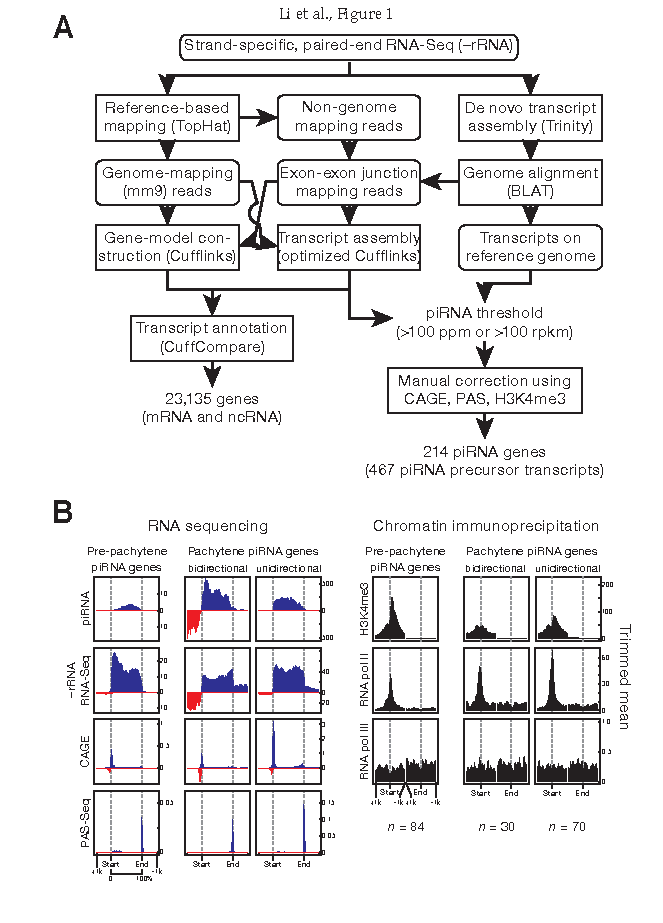
\includegraphics{Figures/Chapter4/MolCel2013_Fig1.pdf}
	\caption[piRNA Precursors are RNA Pol II Transcripts]
	{
	piRNA Precursors are RNA Pol II Transcripts\\[0.25cm]
	(A) Strategy to assemble the mouse testis transcriptome. Rectangles with rounded corners, input or output data; rectangles, processes. Decisions are shown without boxing.(B) Aggregated data for piRNA-producing transcripts (5\% trimmed mean). Oxidized small RNA (>23 nt) sequencing data were used to detect piRNAs; transcript abundance was measured using total RNA depleted of rRNA (RNA-seq). RNA Pol III data were from SRA001030. Dotted lines show the transcriptional start site (Start) and site of polyadenylation (End). See also Figure \ref{fig:MolCelS1}.
	}
	\label{fig:MolCelF1}
\end{figure}
%% ############# FIGURE
%% ############# FIGURE
\begin{figure}[htbp]
	\centering 
	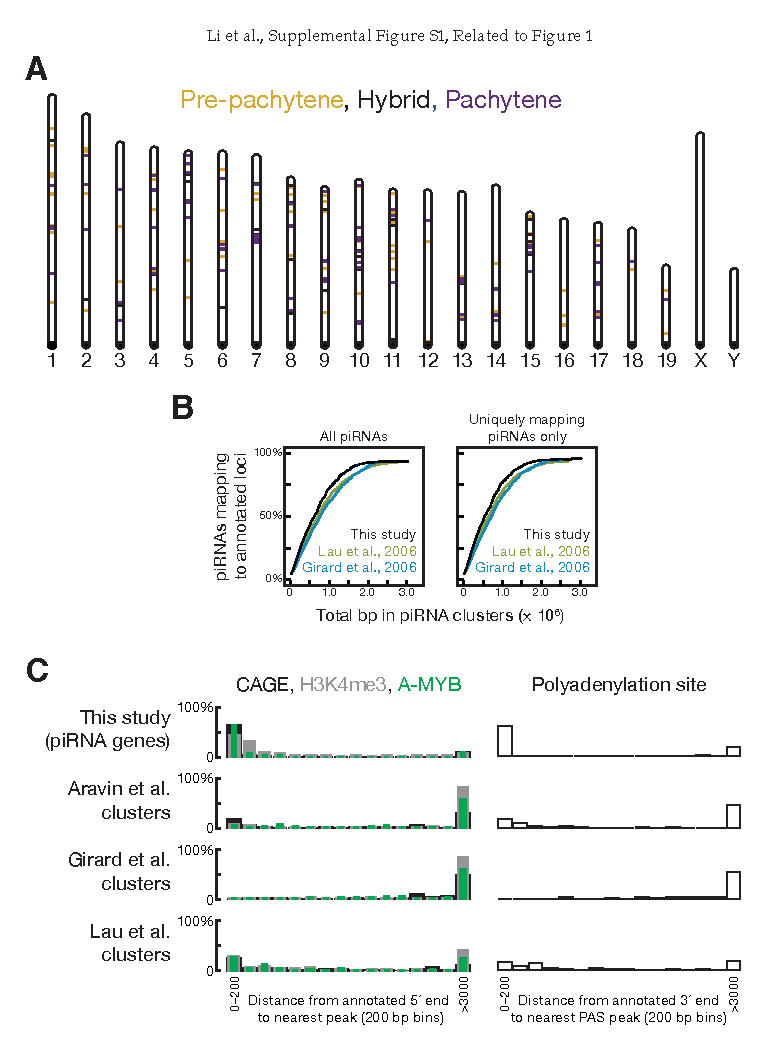
\includegraphics{Figures/Chapter4/MolCel2013_FigS1.pdf}
	\caption[The Major piRNA-Producing Genes of the Post-Partum Mouse Testis]
	{
	(A) Positions of the 214 major piRNA-producing genes on the 19 autosomes of mice. We detected no loci on the X or Y chromosomes. (B) Cumulative distributions for all piRNAs and for uniquely mapping piRNAs comparing the piRNA loci defined by our methods and by previous approaches \citep{Girard2006, Lau2006}. (C) Histogram of distances (in 200 bp bins) from the annotated 5\textprime~ or 3\textprime~ end of a piRNA gene (this study) or cluster to the nearest peak of reads from high-throughput sequencing for transcript 5\textprime~ (CAGE-seq) or 3\textprime~ (PAS-seq) ends, transcription start sites (H3K4me3) or A-MYB binding.
	}
	\label{fig:MolCelS1}
\end{figure}
%% ############# FIGURE

To identify the transcripts that produce piRNAs, we sequenced piRNAs from six developmental stages of mouse testes (10.5 dpp, 12.5 dpp, 14.5 dpp, 17.5 dpp, 20.5 dpp, and adult) and mapped them to the assembled transcripts. The first round of spermatogenesis proceeds synchronously among the tubules of the testis: mouse testes at 10.5 dpp advance no further than the zygotene stage (staging according to \citep{NEBEL1961}; 12.5 dpp to the early pachytene; 14.5 dpp to the middle pachytene; 17.5 to the late pachytene; and 20.5 dpp to the round spermatid stage. For each stage, we prepared two sequencing libraries: one comprising all small RNAs and one in which oxidation was used to enrich for piRNAs by virtue of their 2\textprime-O-methyl-modified 3\textprime~ termini \citep{Ghildiyal2008}.

To qualify as a piRNA-producing transcript, an assembled RNA was required to produce either a sufficiently high piRNA abundance (>100 ppm; parts per million uniquely mapped reads) or density (>100 rpkm; reads per kilobase of transcript per million uniquely mapped reads). These criteria retained both long transcripts producing an abundance of piRNAs and short transcripts generating many piRNAs per unit of length. To refine the termini of each piRNA-producing transcript, we supplemented the RNA-seq data with high-throughput sequencing of the 5\textprime~ ends of RNAs bearing an N(5\textprime~)ppp(5\textprime~)N cap structure (cap analysis of gene expression; CAGE) and the 3\textprime~ ends of transcripts preceding the poly(A) tail (polyadenylation site sequencing; PAS-seq). The assembled piRNA-producing transcripts likely correspond to continuous RNAs in vivo because the CAGE library used to annotate transcript 5\textprime~ ends was constructed after two rounds of poly(A) selection. Thus, the RNA molecules in the library derive from complete transcripts extending from the 5\textprime~ cap to the poly(A) tail (Figure \ref{fig:MolCelF1}B). Conventional 5\textprime~ and 3\textprime~ RACE (rapid amplification of cDNA ends) analysis of piRNA-producing transcripts confirmed the ends of 16 loci (data not shown). To provide additional confirmation of the 5\textprime~ end of each piRNA-producing transcript, we also determined the locations of histone H3 bearing trimethylated lysine 4 (H3K4me3), a histone modification associated with RNA Pol II transcription start sites \cite{Guenther2007}.

%-----------------------------------
%	SUBSECTION 
%-----------------------------------
\subsection{piRNA Precursor RNAs are Canonical RNA Pol II Transcripts}

The presence of 5\textprime~ caps and poly(A) tails and the binding of histone H3K4me3 to the genomic DNA immediately upstream of the transcription start site of each piRNA locus suggest that piRNA transcripts are produced by RNA pol II \ref{fig:MolCelF1}. Moreover, using antibodies to RNA pol II but not RNA pol III, ChIP-seq showed a peak at the transcription start site as well as polymerase occupancy across the entire piRNA gene (Figure \ref{fig:MolCelF1}B; \citep{Kutter2011}. We conclude that piRNA transcripts are conventional RNA pol II transcripts bearing 5\textprime~ caps and 3\textprime~ poly(A) tails.

%-----------------------------------
%	SUBSECTION 2
%-----------------------------------
\subsection{A Transcript-based Set of piRNA Loci}

Our transcriptome assembly yielded 467 piRNA-producing transcripts that define 214 genomic loci (Figure \ref{fig:MolCelS1}A and \hl{Table S1}). Among the \textasciitilde2.2 million distinct piRNA species and \textasciitilde8.8 million piRNA reads from the adult mouse testis, the 214 genomic loci account for 95\% of all piRNAs.

Previous studies defined piRNA clusters based solely on small RNA sequencing data \citep{Girard2006, Lau2006, Aravin2007a}. Our approach differs in that it (1) uses RNA-seq data, whose greater read length facilitates the identification of introns, allowing us to define the architecture of piRNA precursor transcripts and (2) uses CAGE, PAS-seq, and H3K4me3 ChIP-seq data to refine the 5\textprime~ and 3\textprime~ ends of the piRNA transcripts. Consequently, the piRNA loci presented here account for more piRNAs using fewer genomic base pairs than those previously defined (Figures \ref{fig:MolCelS1}B and \ref{fig:MolCelS1}C; \citep{Lau2006, Girard2006}. Our piRNA-producing loci include 41 piRNA loci that escaped previous detection \citep{Girard2006, Lau2006, Aravin2007a}, 37 of which contain introns. The 41 loci account for 2\% of piRNAs at 10.5 dpp and 0.36\% in the adult testis.

%-----------------------------------
%	SUBSECTION 
%-----------------------------------
\subsection{Three Classes of piRNAs During Post-Natal Spermatogenesis}

Mice produce three PIWI proteins: MIWI2 (PIWIL4), which binds piRNAs in perinatal testis \citep{Carmell2007, Aravin2008a}; MILI (PIWIL2), which binds piRNAs at least until the round spermatid stage of spermatogenesis \citep{Kuramochi-Miyagawa2004, Aravin2006, Aravin2007a}; and MIWI (PIWILl), which is first produced during the pachytene stage of meiosis \citep{Deng2002c}. From 10.5 to 20.5 dpp, piRNA abundance increases and longer piRNAs appear, reflecting a switch from MILI-bound piRNAs, which have a 26–27 nt modal length \citep{Montgomery1998, Aravin2006, Aravin2008a, Robine2009}, to MIWI-bound piRNAs, which have a 30 nt modal length (Figure \ref{fig:MolCelS2}A; \citep{Reuter2009, Robine2009}. This switch occurs at the pachytene phase of meiosis. MILI-bound pre-pachytene piRNAs predominate before the onset of pachynema; at the pachytene and round spermatid stages, most piRNAs are MIWI-bound pachytene piRNAs.

We used hierarchical clustering to analyze the change in piRNA abundance from 10.5 to 20.5 dpp for the 214 genes defined by our data (Figures \ref{fig:MolCelF2}A and \ref{fig:MolCelS2}A and \hl{Table S2}). Three types of piRNA-producing genes were identified according to when their piRNAs first accumulate and how their expression changes during spermatogenesis: 84 pre-pachytene, 100 pachytene, and 30 hybrid loci. At 10.5 dpp, the earliest time we evaluated, 84 genes dominate piRNA production (median piRNA abundance per gene = 16 rpkm; Figure \ref{fig:MolCelF2}B). Nearly all (81 out of 84) were congruent with protein-coding genes. The 84 pre-pachytene piRNA genes account for 13\% of piRNAs at 10.5 dpp, but only 0.31\% of piRNAs in the adult testis. Of the pre-pachytene piRNAs accounted for by the 84 loci, 15\% derive from 31 piRNA-producing genes that, to our knowledge, have not previously been described.

%% ############# FIGURE
\begin{figure}[htbp]
	\centering 
	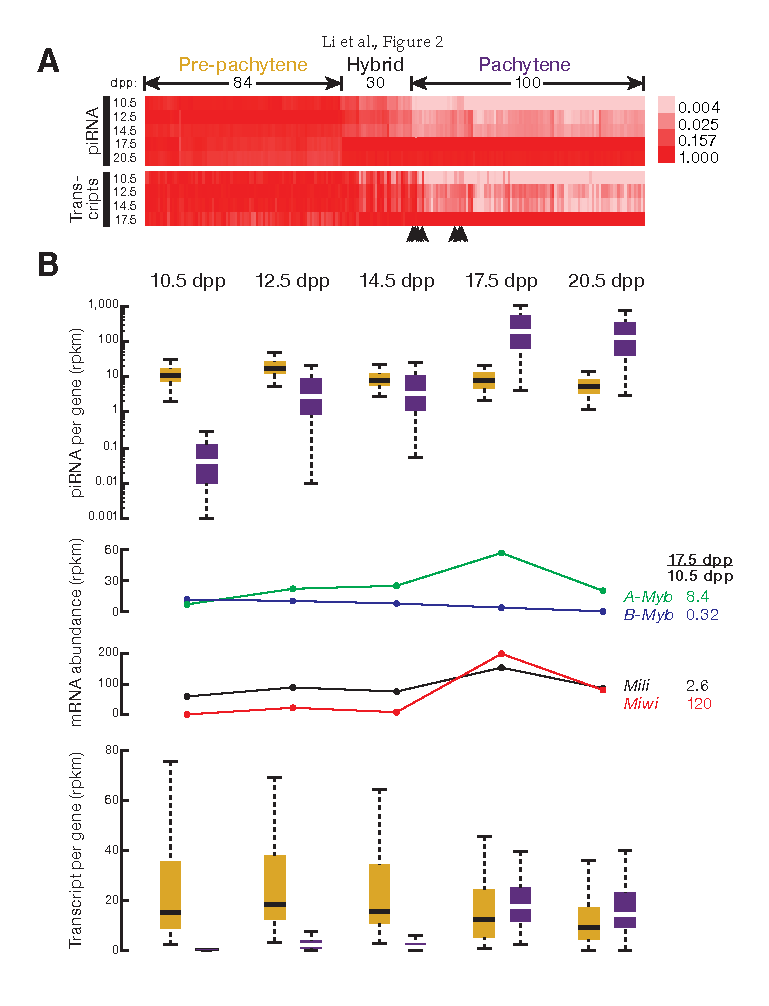
\includegraphics{Figures/Chapter4/MolCel2013_Fig2.pdf}
	\caption[Three Classes of piRNA-Generating Loci]
	{
	(A) Normalized piRNA density (rpkm) for each piRNA-producing gene is shown as a heatmap across the developmental stages. Hierarchical clustering divided the genes into three classes. Arrowheads mark seven pachytene piRNA genes that were not classified as pachytene according to the change in the abundance of their precursor RNAs from 10.5 to 17.5 dpp.(B) Top: box plots present piRNA density per gene as spermatogenesis progresses (here and elsewhere, pre-pachytene in yellow and pachytene in purple). Middle: expression of \amyb{}, \bmyb{}, \mili{}, and \miwi{} was measured by RNA-seq. Bottom: box plots present piRNA precursor expression per gene, measured by RNA-seq, from 10.5 to 20.5 dpp. See also Figure \ref{fig:MolCelS2} and \hl{Table S2}.
	}
	\label{fig:MolCelF2}
\end{figure}
%% ############# FIGURE
%% ############# FIGURE
\begin{figure}[htbp]
	\centering 
	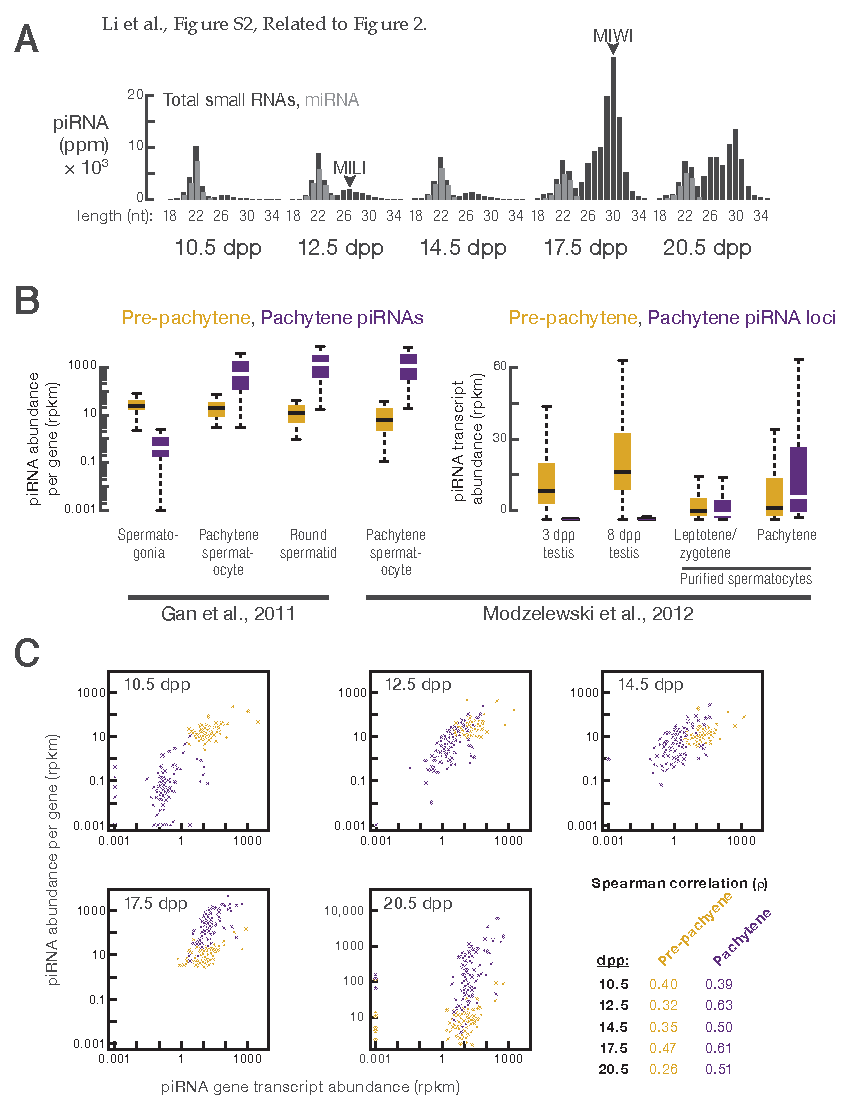
\includegraphics{Figures/Chapter4/MolCel2013_FigS2.pdf}
	\caption[Pre-pachytene piRNAs Persist in Pachytene Spermatocytes]
	{
	(A) As shown previously by others using lower temporal resolution, the modal length of piRNAs increases as spermatogenesis proceeds to more advanced stages. (B) Total piRNA rpkm abundance and piRNA transcript abundance per locus by class, from purified spermatogonia, spermatocytes, round spermatids, and 3 dpp and 8 dpp testis \citep{Gan2011, Modzelewski2012}. (C) Correlation between piRNA abundance per locus and piRNA precursor transcription from 10.5 to 20.5 dpp. Throughout the Figures, gold indicates pre-pachytene and purple indicates pachytene piRNA loci.
	}
	\label{fig:MolCelS2}
\end{figure}
%% ############# FIGURE


A parallel analysis of piRNA precursor transcription using RNA-seq (>100 nt) corroborated the classification based on piRNA abundance; of the 100 piRNA genes classified as pachytene based on the developmental expression profile of their piRNAs, 93 were grouped as pachytene according to the developmental expression profile of their transcripts. Of these 93, 89 are intergenic. All 84 piRNA genes designated pre-pachytene using piRNA data were classified as pre-pachytene according to their transcript abundance.

Despite their name, pre-pachytene piRNAs were readily detected in >90\% and \textasciitilde95\% pure pachytene spermatocytes, as well as round spermatids (Figure \ref{fig:MolCelS2}B; \citep{Gan2011	,Modzelewski2012}. Transcript abundance from the 84 pre-pachytene loci was high at 3 dpp (median abundance = 11 rpkm), higher by 8 dpp (18 rpkm), and lower in purified leptotene/zygotene spermatocytes (3.3 rpkm; \ref{fig:MolCelS2}B). Yet piRNA precursor transcripts were readily detectable in purified pachytene spermatocytes at a level (4.6 rpkm) comparable to that in purified leptotene/zygotene spermatocytes (Figure \ref{fig:MolCelS2}B);  \citep{Gan2011	,Modzelewski2012}. From 10.5 to 20.5 dpp, the steady-state level of pre-pachytene piRNA precursor transcripts remained constant (Figure \ref{fig:MolCelS2}B).

Finally, the abundance of pre-pachytene piRNA precursor transcripts was better correlated with pre-pachytene piRNA abundance at 17.5 dpp ($\rho$ = 0.47), when pachytene spermatocytes compose a larger fraction of the testis, than at 10.5, 12.5, or 14.5 dpp (0.32 $\ge \rho \le$ 0.40; Figure \ref{fig:MolCelS2}C). Our data suggest that the pre-pachytene loci continue to be transcribed and processed into piRNAs long after spermatocytes enter the pachytene stage of meiosis. Thus, the name pre-pachytene piRNA is a misnomer that should be retained only for historical reasons.

Hierarchical clustering identified 100 pachytene genes whose piRNAs emerge at 12.5 dpp, 2 days earlier than previously reported \citep{Girard2006}. Nearly all the pachytene genes are intergenic (93 out of 100). piRNA expression from pachytene piRNA genes peaks at 17.5 dpp (Figure \ref{fig:MolCelF2}B). Overall, the median abundance of piRNAs from these 100 loci increased >6,000-fold from 10.5 to 17.5 dpp. Transcripts from pachytene genes were low at 10.5 dpp (median abundance = 0.15 rpkm) and increased 116-fold from 10.5 to 17.5 dpp. From 10.5 to 20.5 dpp, the dynamics of pachytene piRNA abundance from each piRNA gene correlated with the increase in abundance of its precursor transcripts (0.39 $\ge \rho \le$  0.63; $\rho value \le 7.3 x 10-5$; Figure \ref{fig:MolCelS2}C). The 100 pachytene genes account for 92\% of piRNAs in the adult testis, making it unlikely that biologically functional pachytene piRNAs originate from thousands of genomic loci \citep{Gan2011}. Figures \ref{fig:MolCelF13} and \ref{fig:MolCelS3} provide examples of pachytene and pre-pachytene piRNA genes defined by our data.


%% ############# FIGURE
\begin{sidewaysfigure}[htbp]
	\centering 
	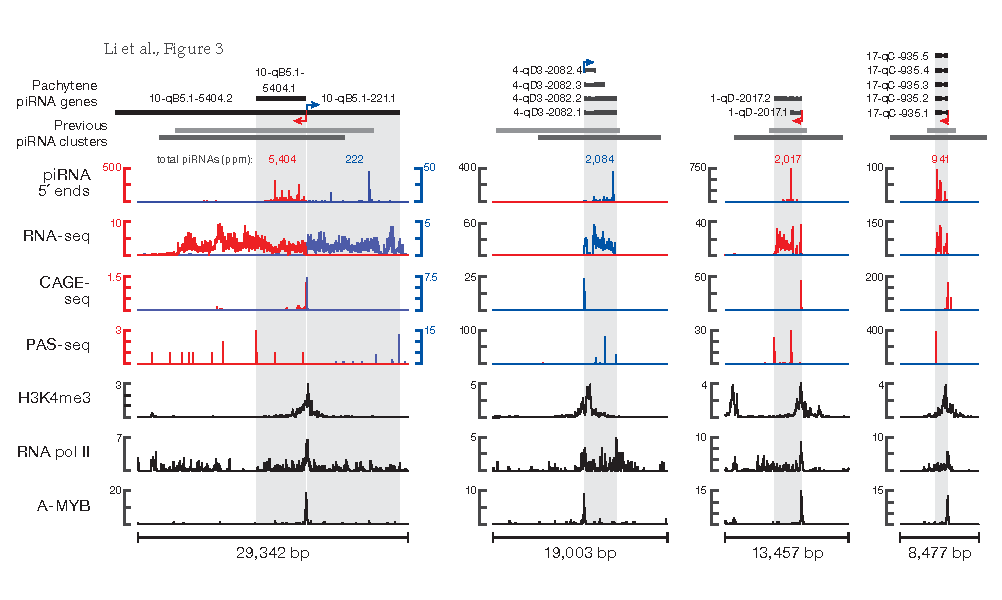
\includegraphics{Figures/Chapter4/MolCel2013_Fig3.pdf}
	\caption[Examples of Pachytene piRNA Genes]
	{
	Previous cluster boundaries are from \citet{Lau2006} in gray and \citet{Girard2006} in  dark gray).
	}
	\label{fig:MolCelF3}
\end{sidewaysfigure}
%% ############# FIGURE
%% ############# FIGURE
\begin{sidewaysfigure}[htbp]
	\centering 
	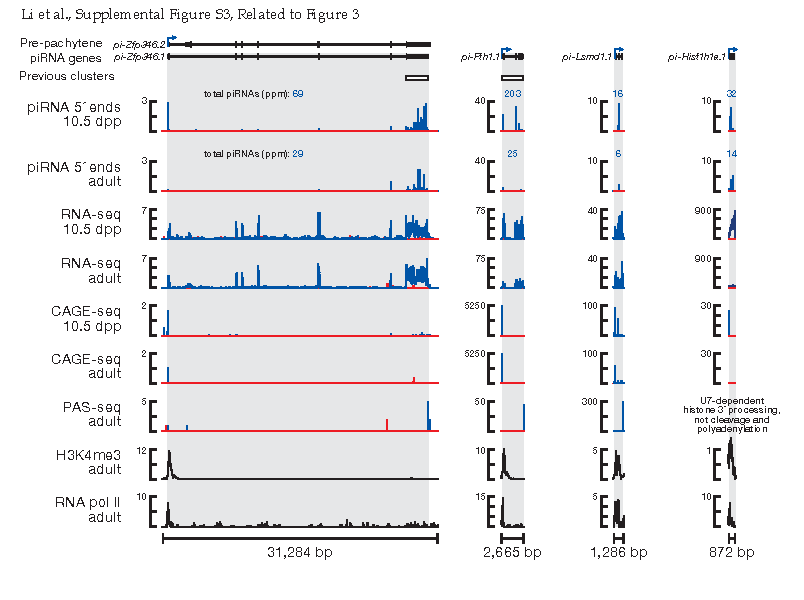
\includegraphics{Figures/Chapter4/MolCel2013_FigS3.pdf}
	\caption[Examples of Pre-Pachytene piRNA Genes]
	{
	Previous cluster boundaries are from \citet{Lau2006} in gray and \citet{Girard2006} in  dark gray).
	}
	\label{fig:MolCelS3}
\end{sidewaysfigure}
%% ############# FIGURE

Hierarchical clustering detected a third class, hybrid piRNAs, which derives from 30 genes with characteristics of both pre-pachytene and pachytene piRNA loci. Like pre-pachytene, hybrid piRNAs were detected at 10.5 dpp (median abundance = 3.7 rpkm) and in purified spermatogonia \citep{Gan2011}. Like pachytene piRNAs, hybrid piRNA abundance increased during the pachytene stage of meiosis, but the increase was delayed until late (17.5 dpp) rather than early pachynema (14.5 dpp). Overall, piRNAs from hybrid genes increased >10-fold from 14.5 to 17.5 dpp. The median abundance of piRNAs from hybrid piRNA genes ranged from 90–120 rpkm in purified pachytene spermatocytes, >20-fold greater than their median abundance in spermatogonia \citep{Gan2011,Modzelewski2012}. Moreover, hybrid piRNA precursor transcripts were readily detected in purified pachytene spermatocytes (median abundance = 9.0 rpkm; \citep{Modzelewski2012}).

%-----------------------------------
%\%	SUBSECTION
%-----------------------------------
\subsection{\amyb{} Regulates Pachytene piRNA Precursor Transcription}

The coordinated increase in pachytene piRNA precursor transcripts suggests their regulation by a common transcription factor or factors. Among the 100 pachytene piRNA genes, 15 pairs (30 genes) are divergently transcribed. The 5\textprime~ ends of the piRNA precursor RNAs from each pair are close in genomic distance (median = 127 bp), suggesting that a shared promoter lies between the two transcription start sites.
 
We took advantage of the unique genomic organization of these 15 pairs of divergently transcribed piRNA genes to search for sequence motifs common to their promoters. The MEME algorithm \citep{Bailey1994} revealed a motif highly enriched in these bidirectional promoters (E = 8.3 x 10$^{12}$; Figure \ref{fig:MolCelF4}A). This motif matches the binding site of the Myb family of transcription factors (Figure \ref{fig:MolCelF4}A; \citep{Gupta2007, Newburger2009}. The Myb motif is not restricted to bidirectional promoters; MEME identified the same motif using the promoters of all pachytene piRNA genes (E = 9.1 x 10$^{-28}$; Figure \ref{fig:MolCelF4}B).


%% ############# FIGURE
\begin{figure}[htbp]
	\centering 
	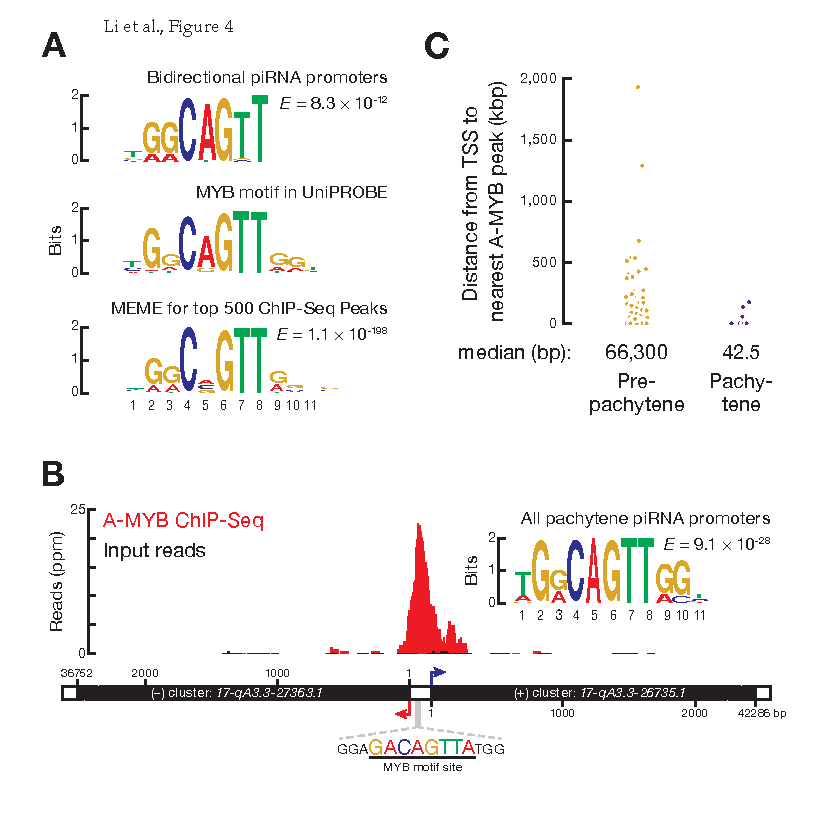
\includegraphics{Figures/Chapter4/MolCel2013_Fig4.pdf}
	\caption[A-MYB Binds the Promoters of Pachytene piRNA Genes]
	{
	 (A) Top: MEME identified a sequence motif in the bidirectional promoters of the 15 pairs of divergently transcribed pachytene piRNA genes. E value computed by MEME measures the statistical significance of the motif. Middle: Myb motif from the mouse UniPROBE database. Bottom: MEME-reported motif for the top 500 (by peak score) A-MYB ChIP-seq peaks from adult mouse testes.(B) A-MYB ChIP-seq data for the common promoter of the divergently transcribed pachytene piRNA genes \textit{17-qA3.3-27363.1} and \textit{17-qA3.3-26735.1}.(C) The distance from the annotated transcription start site (TSS) of each piRNA gene to the nearest A-MYB peak. See also Figure \ref{fig:MolCelS4}.
	}
	\label{fig:MolCelF4}
\end{figure}
%% ############# FIGURE
%% ############# FIGURE
\begin{figure}[htbp]
	\centering 
	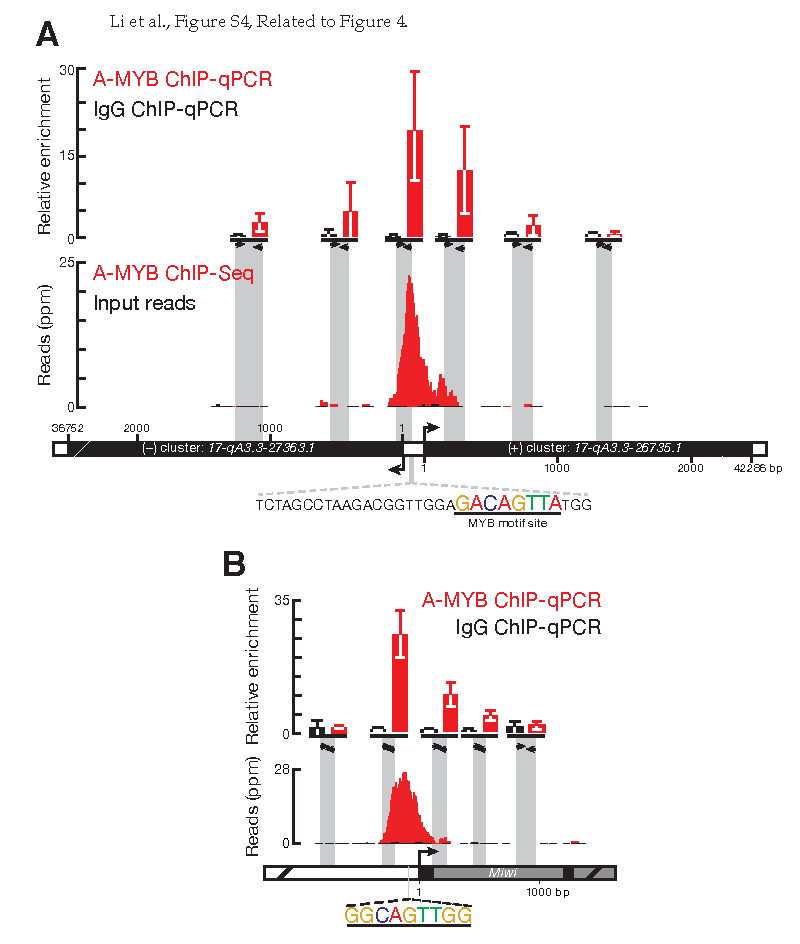
\includegraphics{Figures/Chapter4/MolCel2013_FigS4.pdf}
	\caption[ChIP-qPCR Confirms ChIP-seq Data]
	{
	(A) A-MYB binds to the common promoter of divergently transcribed pachytene piRNA loci \textit{17-qA3.3-27363.1} and \textit{17-qA3.3-26735.1}. The abundance of DNA fragments at the amplified region relative to a control region (mean $\pm$ standard deviation; n = 3) was measured by qPCR (top). The A-MYB ChIP-seq (red) and input (black) data for this pair of genes is presented as in Figure \ref{fig:MolCelF4}B. (B) ChIP-seq and qPCR were as in (A), but for the promoter region of \miwi{} (Piwil1). Also shown is the RefSeq gene model. Exons, black; introns, gray.
	}
	\label{fig:MolCelS4}
\end{figure}
%% ############# FIGURE

The Myb transcription factor family is conserved among eukaryotes. Like other vertebrates, mice produce three Myb proteins, A-MYB (MYBL1), B-MYB (MYBL2), and C-MYB (MYB), each with a distinct tissue distribution \citep{Mettus1994, Trauth1994, Latham1996, Oh1999}. Testes produce both A- and B-MYB proteins. Multiple lines of evidence implicate A-MYB, rather than B-MYB, as a candidate for regulating pachytene piRNA transcription. First, the expression of \amyb{} during spermatogenesis resembles that of pachytene piRNAs: \amyb{} transcripts appear at \textasciitilde12.5 dpp and peak at 17.5 dpp (Figure \ref{fig:MolCelF2}B; \citep{Bolcun-Filas2011}. The expression of \amyb{} messenger RNA (mRNA) increases \textasciitilde15-fold from 8 dpp to 19 dpp, whereas \bmyb{} mRNA expression remains constant and low during the same time frame and into adulthood \citep{Horvath2009}. Our RNA-seq data (Figure \ref{fig:MolCelF2}B) corroborate these findings. Indeed, in our RNA-seq analysis of adult testes, \amyb{} mRNA was 24-fold more abundant than \bmyb{}. Second, a testis-specific \amyb{} point-mutant allele, \mybrepro, which is caused by a cytosine-to-adenine transversion that changes alanine 213 to glutamic acid, leads to meiotic arrest at the pachytene stage with subtle defects in autosome synapsis; \amyb{} null mutant mice have defects in multiple tissues, including the testis and the mammary gland \citep{Toscani1997, Bolcun-Filas2011}. Third, our RNA-seq analysis of \amyb{} mutant testes shows that there is no significant change in \bmyb{} expression in the mutant, compared to the heterozygous controls, at 14.5 or 17.5 dpp. Finally, B-MYB protein is not detectable in pachytene spermatocytes \citep{Horvath2009}.

To assess more directly the role of A-MYB in pachytene piRNA precursor transcription, we used anti-A-MYB antibody to perform ChIP followed by high-throughput sequencing of the A-MYB-bound DNA. The anti-A-MYB antibody is specific for A-MYB, and the peptide used to raise the antibody is not present in B-MYB. The model-based analysis of ChIP-seq (MACS) algorithm \citep{Zhang2008} reported 3,815 genomic regions with significant A-MYB binding (false discovery rate, FDR < 10$^{25}$); we call these regions A-MYB peaks or peaks. Among the 500 peaks with the lowest FDR values, 394 (80\%) contained at least one significant site ($\rho < 10^{4}$) for the MYB binding motif (Figure \ref{fig:MolCelF4}A). Figure \ref{fig:MolCelF4}B shows an example of such an A-MYB peak at the bidirectional promoter of the divergently transcribed pair of pachytene piRNA genes \textit{17-qA3.3-27363.1} and \textit{17-qA3.3-26735.1}. A-MYB occupancy of this genomic site was confirmed by ChIP and quantitative PCR (ChIP-qPCR) (Figure \ref{fig:MolCelS4}A).

The median distance from the transcription start site to the nearest A-MYB peak was \textasciitilde43 bp for the 100 pachytene piRNA genes but >66,000 bp for the 84 pre-pachytene genes (Figure \ref{fig:MolCelF4}C). Our data suggest that during mouse spermatogenesis A-MYB binds to the promoters of both divergently and unidirectionally transcribed pachytene piRNA genes.

To test the idea that A-MYB promotes transcription of pachytene, but not pre-pachytene, piRNA genes, we used RNA-seq to measure the abundance of RNA > 100 nt long from the testes of \amyb{} point-mutant (\mybrepro) mice and their heterozygous littermates (Figure \ref{fig:MolCelF5}). Pachytene piRNA precursor transcripts—both divergently and unidirectionally transcribed—were significantly depleted in \amyb{} mutant testes compared to the heterozygotes: the median decrease was 45-fold at 14.5 dpp (q = 1.1 x 10$^{-13}$) and 248-fold at 17.5 dpp (q = 3.9 x 10$^{-23}$). The abundance of pre-pachytene piRNA transcripts was not significantly changed (q $\ge $ 0.34). The binding of A-MYB to the promoters of pachytene piRNA genes, together with the depletion of pachytene piRNA transcripts in the \amyb{} mutant, further supports the view that A-MYB directly regulates transcription of pachytene piRNA genes.

%-----------------------------------
%	SUBSECTION 2
%-----------------------------------
\subsection{\amyb{} Regulates Pachytene piRNA Production}

To test the consequences of the loss of piRNA precursor transcripts, we measured piRNA abundance in the \amyb{} mutant. Like pachytene piRNA precursor transcription, pachytene piRNA abundance significantly decreased in mutant testes. At 14.5 dpp, median piRNA abundance per pachytene gene decreased 87-fold in \amyb{} homozygous mutant testes compared to heterozygotes ($\rho < 2.2 X 10^{-16}$; Figure \ref{fig:MolCelF5}. By 17.5 dpp, median pachytene piRNA abundance was >9,000 times lower in the \amyb{} mutant than the heterozygotes (P < 2.2 x 10$^{-16}$). In contrast, pre-pachytene piRNA levels were essentially unaltered. Figure 6 presents examples of the effect at 14.5 and 17.5 dpp of the \amyb{} mutant on piRNA precursor transcript and mature piRNA abundance for one pre-pachytene and three pachytene piRNA genes.

%% ############# FIGURE
\begin{figure}[htbp]
	\centering 
	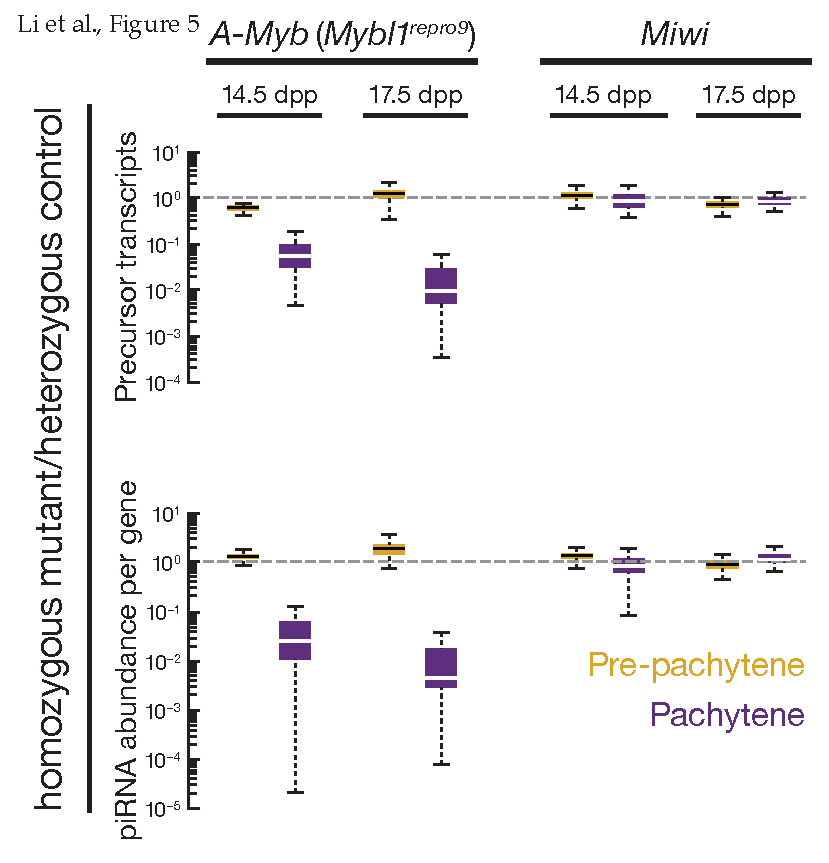
\includegraphics{Figures/Chapter4/MolCel2013_Fig5.pdf}
	\caption[Pachytene piRNAs and Precursors Decrease in \amyb{} Mutant Testes]
	{
	The change in transcript or piRNA abundance per gene in \amyb{} (n = 3) and \miwi{} (n = 1) mutants compared to heterozygotes in testes isolated at 14.5 and 17.5 dpp. See also Figure \ref{fig:MolCelS5}.
	}
	\label{fig:MolCelF5}
\end{figure}
%% ############# FIGURE
%% ############# FIGURE
\begin{figure}[htbp]
	\centering 
	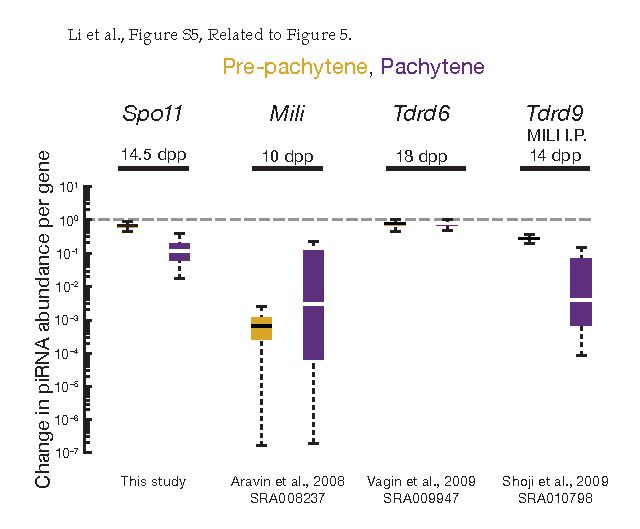
\includegraphics{Figures/Chapter4/MolCel2013_FigS5.pdf}
	\caption[Change in piRNA Expression in \spo{}, \miwi{}, \textit{Tdrd6}, and \textit{Tdrd9} Mutants]
	{
	Change in piRNA abundance per locus (rpkm) for \spo{} (14.5 dpp), \miwi{} (\textit{Piwil2}; 10.5 dpp), \textit{Tdrd6} (18 dpp), and \textit{Tdrd9} (14 dpp) mutants compared to heterozygous controls.
	}
	\label{fig:MolCelS5}
\end{figure}
%% ############# FIGURE

Our data show that A-MYB binds to the promoters of pachytene piRNA genes; \amyb{}, \miwi{}, and pachytene piRNA precursor transcription begins at 12.5 dpp; and \amyb{} mutant spermatocytes reach pachynema with subtle defects in autosome synapsis \citep{Bolcun-Filas2011}. Could pachytene piRNA depletion nonetheless be an indirect consequence of the meiotic arrest caused by the \amyb{} mutant? To test this possibility, we sequenced small RNAs from \spo{} mutant testes, which failed to generate double-stranded DNA breaks at the leptotene stage and display a meiotic arrest \citep{Baudat2000,Romanienko2000}. The median abundance of piRNAs from pre-pachytene genes did not decrease at 14.5 dpp. By 17.5 dpp, piRNA from pachytene genes decreased just 5.9-fold in the \spo{} mutant testes compared to the heterozygotes (Figure \ref{fig:MolCelS5}). We note that A-MYB protein abundance is reduced in the \spo{} mutant \citep{Bolcun-Filas2011}.

\textit{Trip13} is required to complete the repair of double-strand DNA breaks on fully synapsed chromosomes. \textit{Trip13} mutants display a meiotic arrest similar to that in \amyb{} mutant testes \citep{Li2007}: pachytene arrest with synapsed chromosomes. To further test whether the loss of pachytene piRNA precursor transcripts in \amyb{} mutants reflects a general effect of meiotic arrest, we measured piRNA precursor transcript abundance in \textit{Trip13} mutant testes at 17.5 dpp. Unlike \amyb{}, piRNA precursor transcripts were readily detectable in the \textit{Trip13} mutant (Figure \ref{fig:MolCelS6}). We conclude that the loss of pachytene piRNA precursor transcripts and piRNAs in \amyb{} mutant testes is a direct consequence of the requirement for A-MYB to transcribe pachytene piRNA genes and not a general feature of meiotic arrest at the pachytene stage.

%-----------------------------------
%	SUBSECTION 2
%-----------------------------------
\subsection{\amyb{} Regulates Expression of piRNA Biogenesis Factors}

The \amyb{} mutant more strongly affected pachytene piRNA accumulation than it did the steady-state abundance of the corresponding piRNA precursor transcripts (Figure \ref{fig:MolCelF5}; the median decrease in pachytene piRNA abundance was 2-fold greater at 14.5 dpp and 38-fold greater at 17.5 dpp than the decrease in the steady-state abundance of pachytene precursor transcripts \hl{(Table S1)}. These data suggest that A-MYB exerts a layer of control on piRNA accumulation beyond its role in promoting pachytene piRNA precursor transcription.

\miwi{} has previously been proposed to be a direct target of A-MYB; \miwi{} mRNA abundance is reduced in A-MYB mutant testes, and ChIP microarray data place A-MYB on the \miwi{} promoter \citep{Bolcun-Filas2011}. Our RNA-seq data confirm that accumulation of \miwi{} mRNA requires A-MYB: \miwi{} mRNA decreased more than 50-fold in testes isolated from \amyb{} mutant mice at 14.5 dpp compared to their heterozygous littermates (Figures \ref{fig:MolCelF7}A and \ref{fig:MolCelS7} and \hl{Table S3}). Furthermore, our ChIP data confirm that A-MYB binds the \miwi{} promoter in vivo (Figures \ref{fig:MolCelF7}B, \ref{fig:MolCelS4}B, and \ref{fig:MolCelS7}). Like pachytene piRNAs, \miwi{} transcripts first appear at 12.5 dpp (Figure \ref{fig:MolCelF2}B), and MIWI protein is first detected in testes at 14.5 dpp \citep{Deng2002}. Loss of MIWI arrests spermatogenesis at the round spermatid stage \citep{Deng2002}.



A previous study reported that piRNAs fail to accumulate to wild-type levels in \miwi{} mutant testes \citep{Grivna2006b}. However, our data suggest that the overall change in piRNA abundance caused by loss of MIWI is quite small: RNA-seq detected no change at 14.5 dpp (change in total piRNA abundance = 1.1; n = 2) and only a modest decrease at 17.5 dpp (change in total piRNA abundance = 0.58; n = 1). piRNAs from pachytene loci decreased just 2.7-fold at 14.5 dpp (p = 0.0046) and 3.5-fold at 17.5 dpp (p = 1.8 x 10-6) in \miwi{} mutant testes (Figure \ref{fig:MolCelF5}). By comparison, pachytene piRNAs declined 87-fold at 14.5 dpp and 9,400-fold at 17.5 dpp in the \amyb{} mutant.

Does the loss of MIWI affect piRNA precursor transcription? We measured transcript abundance and piRNA expression in \miwi{} null mutant testes at 14.5 and 17.5 dpp. In \miwi{}$^{-/-}$ testes, pachytene piRNA precursor transcripts were present at levels indistinguishable from \miwi{} heterozygotes (median change = 1.0- to 1.4-fold; q = 1; Figure \ref{fig:MolCelF5}). Thus, loss of MIWI does not explain loss of pachytene piRNA precursor transcripts in \amyb{} mutant testes.

%% ############# FIGURE
\begin{figure}[htbp]
	\centering 
	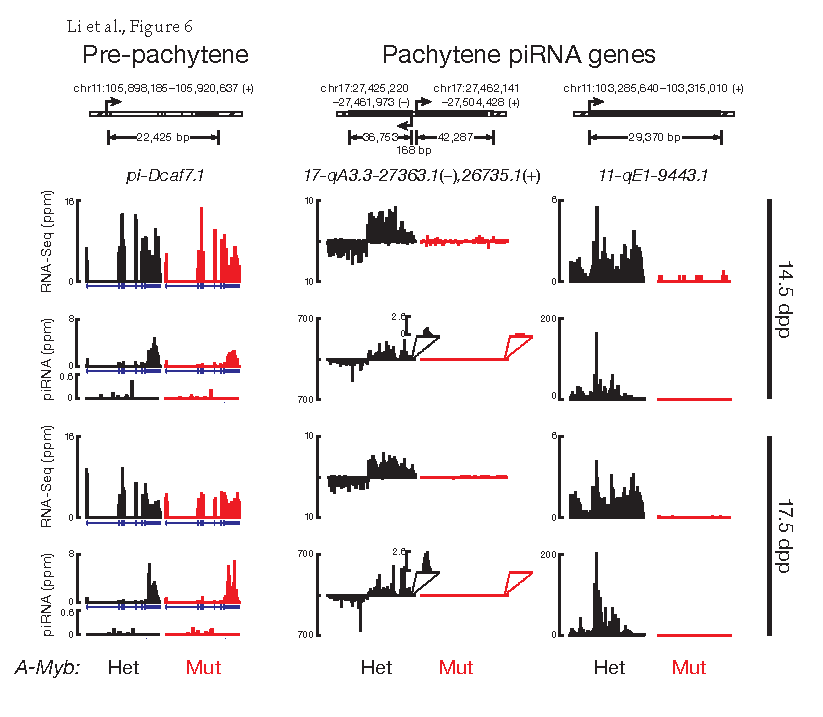
\includegraphics{Figures/Chapter4/MolCel2013_Fig6.pdf}
	\caption[Examples of the Effect of the \amyb{} Mutation on piRNA Expression]
	{
	Transcript and piRNA abundance in heterozygous (Het) and homozygous \amyb{} (Mut) point-mutant testes is shown for four illustrative examples at 14.5 and 17.5 dpp. Also shown is the abundance of piRNA sequencing reads that map to the exon-exon junctions. Gene \textit{11-qE1-9443} does not have an intron. Exons, blue boxes; splice junctions, gaps; the last exon is compressed and not to scale. See also Figure \ref{fig:MolCelS6}.
	}
	\label{fig:MolCelF6}
\end{figure}
%% ############# FIGURE

%% ############# FIGURE
\begin{figure}[htbp]
	\centering 
	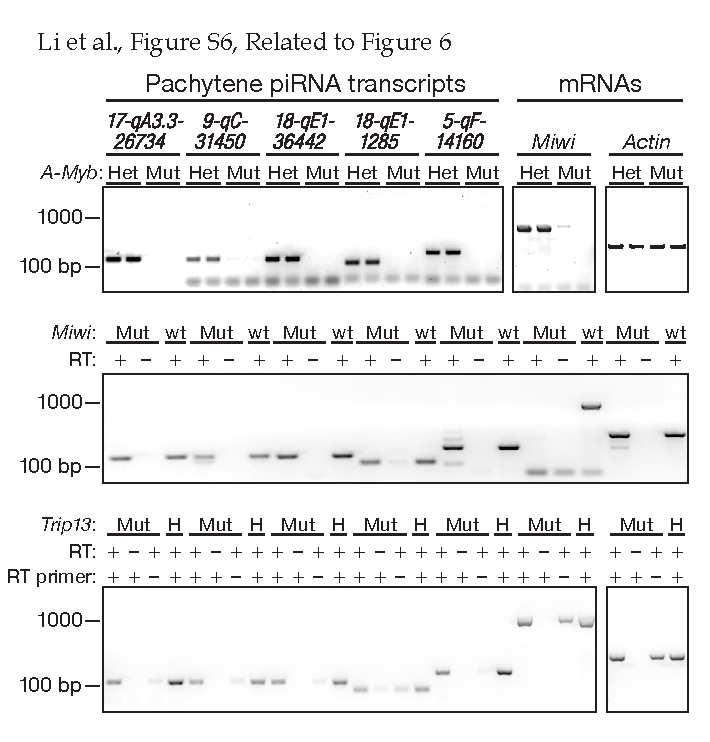
\includegraphics{Figures/Chapter4/MolCel2013_FigS6.pdf}
	\caption[Pachytene piRNA Precursor Abundance in \amyb{}, \miwi{}, and \textit{Trip13} Mutants]
	{
	Transcripts were detected in total RNA from adult testes by RT-PCR (using random primers) for five pachytene piRNA loci as well as \miwi{} and \textit{Actin}. Mut, mutant; Het or H, heterozygote; wt, wild type.
	}
	\label{fig:MolCelS6}
\end{figure}
%% ############# FIGURE

In addition to \miwi{}, ChIP-seq detected A-MYB bound to the promoters of 12 other RNA-silencing-pathway genes (Figure \ref{fig:MolCelF7}B and \hl{Table S3}). Of these, the mRNA abundance—measured by three biologically independent RNA-seq experiments—of \textit{Ago2}, \textit{Ddx39} (uap56 in flies), \textit{Mael}, \mili{}, \textit{Mov10l1}, \textit{Tdrd9}, and \textit{Vasa} did not change significantly at 14.5 dpp in \amyb{} mutant testes compared to heterozygotes (q > 0.05); except for \textit{Ago2}, all decreased significantly in the mutant at 17.5 dpp. In contrast, the abundance of the mRNAs encoding Tudor domain proteins decreased significantly in \amyb{} mutant testes: \textit{Tdrd6} (64-fold decrease; q = 3.1 x 10-5) and \textit{Tdrd5} (7.5-fold decrease; q = 1.0 x 10-5). \textit{Tdrd5} is expressed in embryonic testes then decreases around birth \citep{Yabuta2011}. \textit{TDRD5} protein reappears at 12 dpp, increasing throughout the pachynema \citep{Smith2004, Yabuta2011}. Our data indicate that A-MYB activates \textit{Tdrd5} transcription at the onset of the pachytene stage of meiosis. Similarly, \textit{Tdrd6} mRNA can be detected at the middle pachytene, but not the zygotene stage, and peaks after late pachytene; TDRD6 protein can be detected at 17 dpp and continues to increase until 21 dpp \citep{Vasileva2009}. The findings that TDRD5 and TDRD6 colocalize with MIWI in pachytene spermatocytes \citep{Hosokawa2007, Vasileva2009, Yabuta2011} and that TDRD6 binds MIWI \citep{Chen2009a, Vagin2009, Vasileva2009} suggest a role for these Tudor domain proteins in pachytene piRNA production or function. As in \miwi{}-/- testes, spermatogenesis arrests at the round spermatid stage in \textit{Tdrd5}$^{-/-}$ and \textit{Tdrd6}$^{-/-}$ mutant testes \citep{Vasileva2009, Yabuta2011}. Loss of \textit{Tdrd6} expression has little effect on piRNA levels (Figure \ref{fig:MolCelS3}; \citep{Vagin2009}, perhaps because the functions of Tudor domain proteins overlap.

Other genes encoding piRNA pathway proteins whose promoters are bound by A-MYB and whose expression decreased significantly in \amyb{} mutant testes include \textit{MitoPld} (\textit{Pld6}; 3.9-fold decrease; q = 0.0095) and \textit{Tdrd12} (5.3-fold decrease; q = 0.0046). \textit{MitoPld} encodes an endoribonuclease implicated in an early step in piRNA biogenesis in mice and flies \citep{Houwing2007, Pane2007, Haase2010, Huang2011, Watanabe2011a, Ipsaro2012, Nishimasu2012}. The function of Tdrd12 is not known, but its fly homologs (Yb, Brother of Yb, and Sister of Yb) are all required for piRNA production \citep{Handler2011}. \textit{Tdrd1} decreased 3.4-fold, but with q value = 0.015. \textit{Tdrd1} is first expressed in fetal prospermatogonia, then re-expressed in pachytene spermatocytes \citep{Chuma2006a}. In Tdrd1 mutant testes, spermatogenesis fails, with no spermatocytes progressing past the round spermatid stage \citep{Chuma2006a}. TDRD1 binds MILI and MIWI \citep{Chen2009a, Kojima2009} and colocalizes with TDRD5 and TDRD6 in the chromatoid body \citep{Hosokawa2007}.

Together, these data support the idea that at the onset of the pachytene phase of meiosis, A-MYB coordinately activates transcription of many genes encoding piRNA pathway proteins.

%-----------------------------------
%	SUBSECTION 2
%-----------------------------------
\subsection{A-MYB and the Pachytene piRNA Regulatory Circuitry}

A number of genes encoding known and suspected piRNA pathway proteins are bound and regulated by A-MYB (Figures \ref{fig:MolCelF7}B and \ref{fig:MolCelS7}C). Our data support a model in which A-MYB drives both the transcription of pachytene piRNA genes and the mRNAs encoding genes required for piRNA production including \miwi{}, \textit{MitoPld}, and \textit{Tdrd9}. Regulation by A-MYB of both the sources of pachytene piRNAs and the piRNA biogenesis machinery creates a coherent feedforward loop (Figure \ref{fig:MolCelF7}C). Feedforward loops amplify initiating signals to increase target gene expression. Furthermore, they function as switches that are sensitive to sustained signals; they reject transient signals \citep{Shen-Orr2002, Osella2011}. 

A-MYB also bound to the \amyb{} promoter (Figure \ref{fig:MolCelF7}B), and \amyb{} transcripts decreased 4.2-fold in testes from an \amyb{} point mutant (\mybrepro{}; Figure \ref{fig:MolCelF7}B). The \amyb{} mutant fails to produce the high level of A-MYB protein observed in wild-type testes at the late pachytene stage of meiosis \citep{Bolcun-Filas2011}. Instead, A-MYB protein never becomes more abundant than the level achieved in wild-type testes by the beginning of the pachytene stage. While the lower level of A-MYB in the \amyb{} mutant may reflect instability of the mutant protein, a simpler explanation is that mutant A-MYB cannot activate \amyb{} transcription.

%% ############# FIGURE
\begin{figure}[htbp]
	\centering
	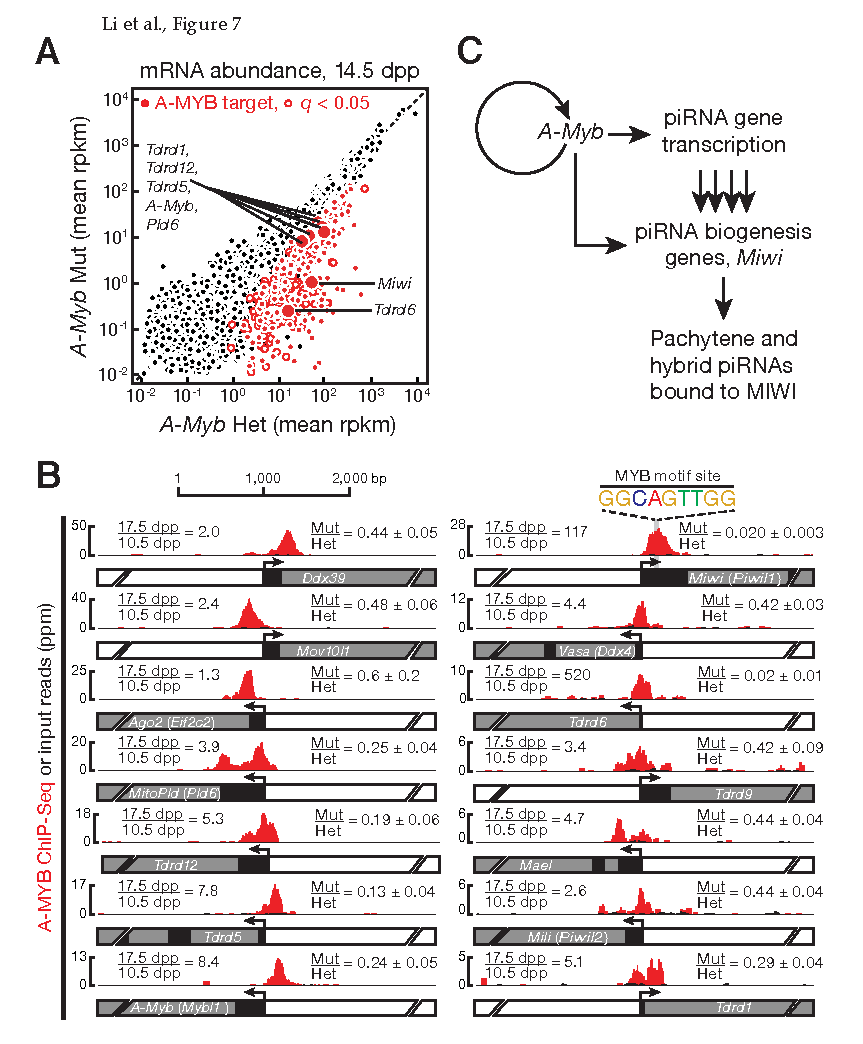
\includegraphics{Figures/Chapter4/MolCel2013_Fig7.pdf}
	\caption[A-MYB Regulates Expression of mRNAs Encoding piRNA Pathway Proteins]
	{
	(A) mRNA abundance in \amyb{} mutant versus heterozygous testes. The 407 genes with a significant (q < 0.05) change in steady-state mRNA levels are shown as red circles. The 203 with A-MYB peaks within 500 bp of their transcription start site are filled.
	(B) A-MYB ChIP-seq signal at the transcription start sites of \amyb{} and genes implicated in RNA silencing pathways. For each, the figure reports the change in mRNA abundance between 17.5 and 10.5 dpp in wild-type testes and the mean change between \amyb{} mutant and heterozygous testes at 14.5 dpp (mean $\pm$ SD; n = 3).
	(C) A model for the regulation of pachytene piRNA biogenesis by A-MYB. See also Figure \ref{fig:MolCelS7} and \hl{Table S3}.
	}
	\label{fig:MolCelF7}
\end{figure}
%% ############# FIGURE

%% ############# FIGURE
\begin{figure}[htbp]
	\centering 
	\includegraphics{Figures/Chapter4/MolCel2013_FigS7.pdf}
	\caption[\amyb{} mutants, but Not \miwi{} Mutants, Change the Expression of RNA Silencing Pathway Genes]
	{
	A) mRNA abundance in 17.5 dpp \amyb{} versus heterozygous testes. The 2,853 genes with a significant (q < 0.051) change in steady-state mRNA abundance are shown as open red circles. Among them, 8721,009 genes also had A-MYB peaks within 500 bp of their transcription start sites. These “A-MYB targets” are marked with filled red circles. (B) Same as (A) but in 14.5 dpp \miwi{} mutant versus heterozygous testes. The genes encoding proteins implicated in RNA silencing pathways that were labeled in (A) and that showed no change in expression in \miwi{} mutant testes are highlighted as green filled circles. As expected, \miwi{}, showed a significant decrease in mRNA abundance in \miwi{}-/- testes. (C) The change in mRNA abundance (rpkm) in \amyb{} and \miwi{} mutant testes versus heterozygous controls for the RNA silencing genes highlighted in (A) and (B).
	}
	\label{fig:MolCelS7}
\end{figure}
%% ############# FIGURE

%-----------------------------------
%	SUBSECTION 
%-----------------------------------
\subsection{Feed-Forward Regulation of piRNA Production is Evolutionarily Conserved}

Is A-MYB-mediated, feedforward control a general feature of regulation of piRNA production among vertebrates? To test whether A-MYB control of piRNA precursor transcription is evolutionarily conserved, we used high-throughput sequencing to identify piRNAs in adult rooster testes. Birds and mammals diverged 330 million years ago \citep{Benton2007}. After removing the sequences of identifiable miRNAs \citep{Burnside2008} and annotated noncoding RNAs, total small RNA from the adult rooster testis showed peaks at both 23 and 25 nt (Figure \ref{fig:MolCelF8}A). When the RNA was oxidized before being prepared for sequencing, only a single 25 nt peak remained, consistent with the 25 nt small RNAs corresponding to piRNAs containing 2\textprime-O-methyl-modified 3\textprime~ termini. These longer, oxidation-resistant species typically began with uracil (62\% of species and 65\% of reads; Figure \ref{fig:MolCelF8}B), and we detected a significant Ping-Pong amplification signature (Z score = 31; Figure \ref{fig:MolCelF8}C). We conclude that the oxidation-resistant, 24–30 nt long small RNAs correspond to rooster piRNAs. Like piRNAs generally, rooster piRNAs are diverse, with 5,742,529 species present among 81,121,893 genome-mapping reads. Like mouse pachytene piRNAs, 70\% of piRNAs from adult rooster testes mapped to unannotated intergenic regions, 19\% mapped to transposons, and 14\% mapped to protein-coding genes. Of the piRNAs that map to protein-coding genes, >95\% derive from introns. Forty-two percent of piRNA species mapped uniquely to the Gallus gallus genome.

Using 24–30 nt piRNAs from oxidized libraries, we identified 327 rooster piRNA clusters (Figure \ref{fig:MolCelS8}). These account for 76\% of all uniquely mapping piRNAs. Of the 327 clusters, 25 overlapped with protein-coding genes. To begin to identify the transcription start sites for the rooster piRNA clusters, we analyzed adult rooster testes by H3K4me3 ChIP-seq. More than 81\% (268 out of 327) of the clusters contained a readily detectable H3K4me3 peak within 1 kbp of the piRNA cluster. In contrast, the median distance from a cluster to the nearest transcription start site of an annotated gene was 73 kbp, suggesting that the H3K4me3 peaks reflect the start sites for rooster piRNA precursor transcripts.

Next, we asked where in the genome A-MYB bound in adult rooster testes. A-MYB ChIP-seq identified 5,509 significant peaks (FDR < 10-25). MEME analysis of the top 500 peaks with the lowest FDR values identified a motif (E = 2.6 x 10-201; Figure \ref{fig:MolCelF8}D) similar to that found in the mouse (Figure \ref{fig:MolCelF4}A). A-MYB is the only one of the three chicken MYB genes expressed in adult testis (X.Z.L. and P.D.Z., unpublished data), supporting the view that these peaks correspond to A-MYB binding. The core sequence motif associated with A-MYB binding in mouse differs at one position (CAGTT) from that in rooster (C C/G GTT). This difference between mammalian and chicken MYB proteins has been noted previously \citep{Weston1992, Deng1996}.

%% ############# FIGURE
\begin{figure}[htbp]
	\centering 
	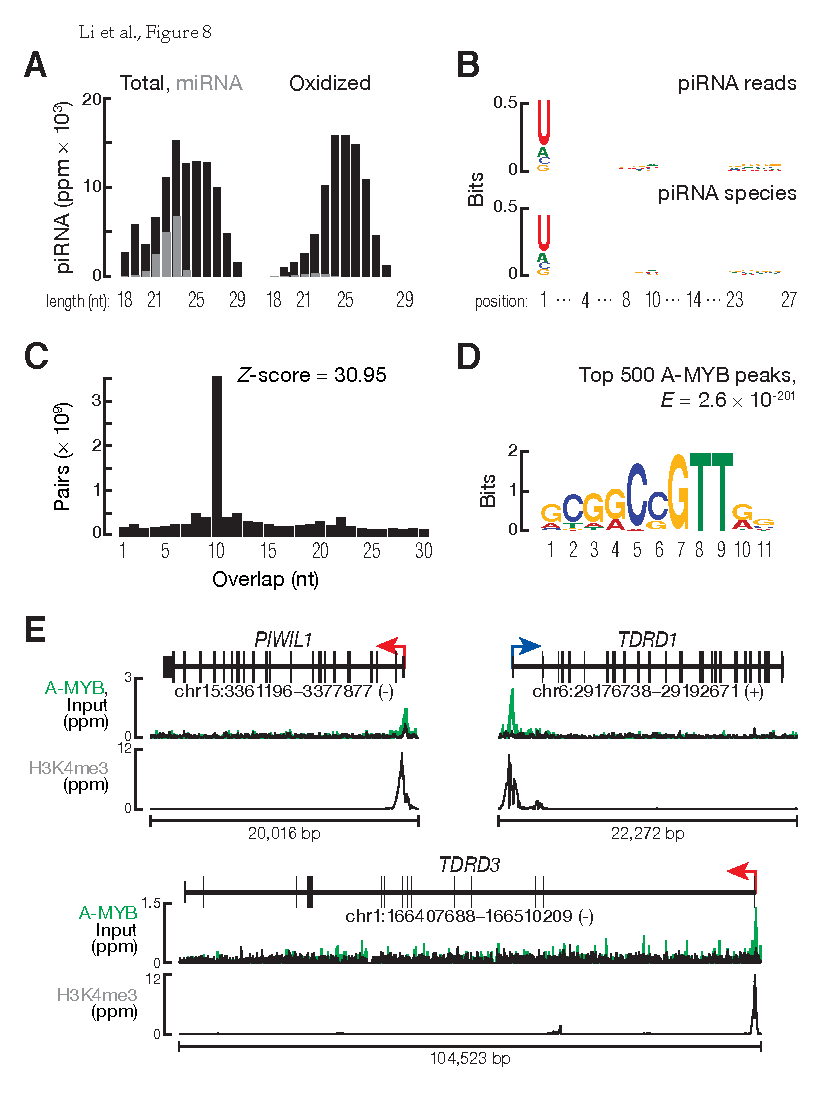
\includegraphics{Figures/Chapter4/MolCel2013_Fig8.pdf}
	\caption[Feed-Forward Regulation of piRNA Biogenesis by A-MYB is Conserved in Rooster]
	{
	(A) Length distributions of total rooster testis small RNAs (black) and miRNAs (gray).(B) Sequence logo showing the nucleotide composition of piRNA reads and species.(C) The 5\textprime~-5\textprime~ overlap between piRNAs from opposite strands was analyzed to determine if rooster piRNAs display Ping-Pong amplification. The number of pairs of piRNA reads at each position is reported. Z score indicates that a significant 10 nt overlap (Ping-Pong) was detected. Z score > 1.96 corresponds to p value < 0.05.(D) MEME-reported motif of the top 500 (by peak score) A-MYB ChIP-seq peaks from adult rooster testes.(E) A-MYB, H3K4me3, and input ChIP-seq signals at the transcription start sites of rooster PIWIL1, TDRD1, and TDRD3. See also Figure S8.
	}
	\label{fig:MolCelF8}
\end{figure}
%% ############# FIGURE

%% ############# FIGURE
\begin{figure}[htbp]
	\centering 
	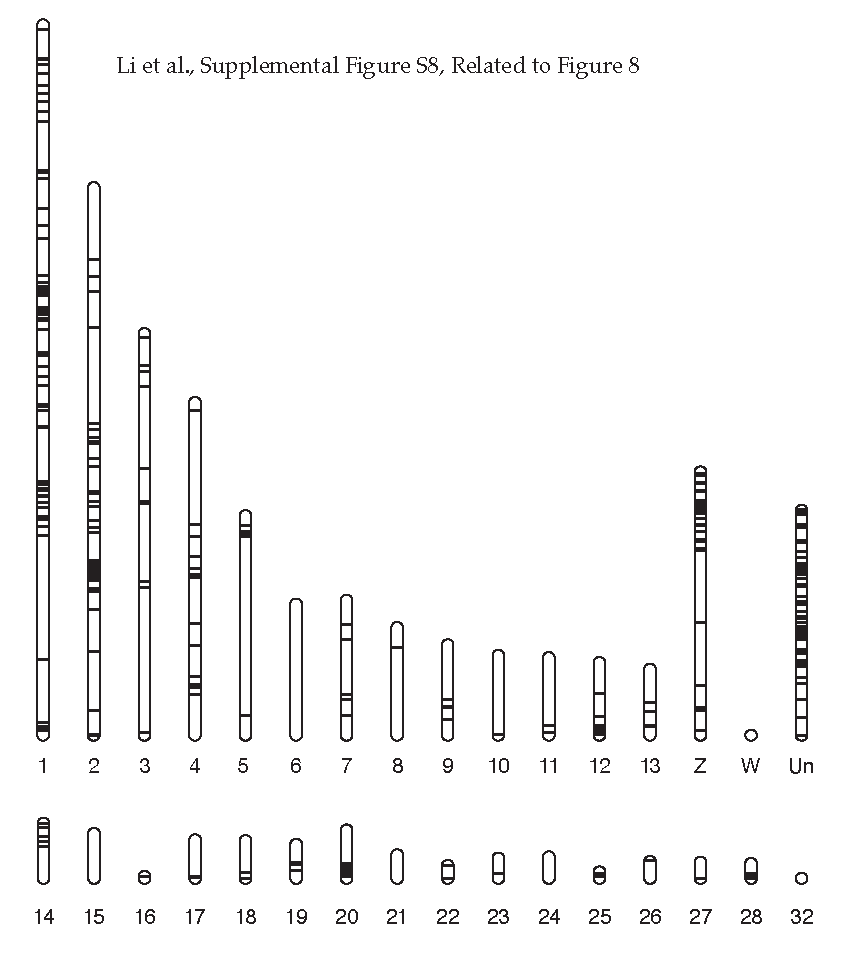
\includegraphics{Figures/Chapter4/MolCel2013_FigS8.pdf}
	\caption[Genomic Locations of piRNA Clusters in the Rooster (Gallus gallus) Testis.]
	{
	Black horizontal lines denote the locations on the Gallus gallus (galGal3) chromosomes of the piRNA clusters identified by small RNA sequencing. The figure shows 324 clusters; clusters on E64 (cluster 370) and E22C19W28_E50C23 (clusters 109 and 563) are not shown.
	}
	\label{fig:MolCelS8}
\end{figure}
%% ############# FIGURE

To determine whether chicken A-MYB might regulate transcription of some piRNA clusters in the testis, we compared the A-MYB peak nearest to each piRNA cluster with the nearest H3K4me3 peak. Of the 327 rooster piRNA clusters, at least 104 were occupied by A-MYB at their promoters, as defined by an overlapping H3K4me3 peak. These 104 clusters account for 31\% of uniquely mapping rooster piRNAs.

The chicken genome encodes at least two PIWI proteins: PIWIL1 and PIWIL2. Remarkably, the promoter of Gallus gallus PIWIL1, the homolog of mouse \miwi{}, contained a prominent A-MYB peak (Figure \ref{fig:MolCelF8}E). TDRD1 and TDRD3 also showed A-MYB peaks (Figure \ref{fig:MolCelF8}E). Thus, as in mice, Gallus gallus A-MYB controls the transcription of both piRNA clusters and genes encoding piRNA pathway proteins. We conclude that A-MYB-mediated feedforward regulation of piRNA production was likely present in the last common ancestor of birds and mammals.

In mice, we found no piRNA-producing genes on the sex chromosomes (Figure \ref{fig:MolCelS1}A), perhaps because mouse sex chromosomes are silenced during the pachytene stage \citep{Li2009d}. Birds use a ZW rather than an XY mechanism for sex determination, so roosters are homogametic (ZZ), allowing the sex chromosomes to remain transcriptionally active in males \citep{Namekawa2009, Schoenmakers2009}. Indeed, we find that 39 of the 327 rooster piRNA clusters are on the Z chromosome, accounting for 12\% of uniquely mapping piRNAs (Figure \ref{fig:MolCelS8}). Of the 39 Z chromosome clusters, 18 had an A-MYB peak at their promoter.

%----------------------------------------------------------------------------------------
%	SECTION 3
%----------------------------------------------------------------------------------------
\section{DISCUSSION}

The data presented here provide strong support for the view that piRNAs in mammals begin as long, single-stranded precursors generated by testis-specific, RNA Pol II transcription of individual piRNA genes (see also \citet{Vourekas2012}. Transcription by RNA Pol II affords piRNA genes the same rich set of transcriptional controls available to regulate mRNA expression. Our data establish that developmentally regulated transcription of piRNA genes determines when specific classes of piRNAs emerge during spermatogenesis.

During mouse spermatogenesis, transcription of pachytene piRNA genes begins at the onset of the pachytene stage of meiosis; pachytene piRNAs accumulate subsequently. The presence of the MYB binding motif near the transcription start sites of pachytene piRNA genes, the physical binding of A-MYB to those genes, and the loss of pachytene piRNA precursor transcripts and piRNAs in testes from \amyb{} mutant mice all argue that A-MYB regulates pachytene piRNA production.

A-MYB also drives increased expression of piRNA pathway genes. Among these, \miwi{} expression shows the greatest dependence on A-MYB, but A-MYB also drives transcription of genes encoding other proteins in the piRNA pathway, including MitoPld, Mael, and five genes encoding Tudor domain proteins. For example, A-MYB increases expression of Tdrd6 more than 500-fold. Loss of A-MYB function more strongly depletes pachytene piRNAs than loss of MIWI, in part because pachytene piRNAs can still be loaded into MILI in \miwi{} mutant testes, although MILI-loaded pachytene piRNAs do not suffice to produce functional sperm. In the \amyb{} mutant, expression of mRNAs encoding multiple piRNA pathway proteins decreases. We speculate that in wild-type male mice, the increased expression of these mRNAs at the onset of the pachytene stage of meiosis ensures that sufficient piRNA-precursor-processing and MIWI-loading factors are available to cope with the large increase in pachytene piRNA precursor transcription.

We propose that induction of A-MYB during the early pachytene stage of spermatogenesis initiates a feedforward loop that ensures the precisely timed production of these piRNAs. Coherent feedforward loops show delayed kinetics in order to reject background stimuli \citep{Mangan2003}. Indeed, we observed a delay from the early to middle pachytene in the accumulation of pachytene piRNAs, despite the continued increase in \amyb{} expression (Figure \ref{fig:MolCelF2}A). Pachytene piRNA levels increase 75-fold (median for the 100 genes) from 10.5 to 12.5 dpp, coincident with increased expression of \amyb{}. However, from 12.5 to 14.5 dpp, pachytene piRNAs increase only 1.2-fold. Pachytene piRNAs subsequently resume their accumulation, increasing 65-fold from 14.5 to 17.5 dpp. We believe this delay is a consequence of a feedforward loop that ensures the production of pachytene piRNAs only at the pachytene stage of spermatogenesis. Regulation by a feedforward loop also predicts a rapid shutdown of pachytene piRNA pathways at round spermatid stage VIII, when A-MYB protein levels decrease \citep{Horvath2009}. Supporting this idea, the abundance of MIWI decreases sharply by the elongated spermatid stage of spermatogenesis \citep{Deng2002}. Testing this proposal is a clear challenge for the future.

In fruit flies and zebrafish \citep{Brennecke2007, Houwing2007}, most piRNAs map to repetitive regions, whereas in mammals, uniquely mapping intergenic piRNAs predominate in the adult testis. The discovery that 70\% of rooster piRNA reads map to intergenic regions suggests that the expansion of intergenic piRNAs controlled by A-MYB feedforward regulation arose before the divergence of birds and mammals. In the future, detailed analysis of piRNA production across avian spermatogenesis should provide insight into the evolutionary origins and functions of pachytene piRNAs, a class of piRNAs thus far only detected in mammals.

In summary, we have shown that mouse piRNA genes are coregulated transcriptionally, establishing that A-MYB coordinately regulates the biogenesis of an entire piRNA class, the pachytene piRNAs. The discovery that a loss-of-function \amyb{} mutant, \mybrepro{}, disrupts piRNA precursor transcription in vertebrates provides a tool to understand the transformation of long, single-stranded piRNA precursors into mature piRNAs and to explore the functions and targets of the pachytene piRNAs.

%----------------------------------------------------------------------------------------
%	SECTION 4
%----------------------------------------------------------------------------------------
\section{EXPERIMENTAL PROCEDURES}

\begin{description}
  \item[Mice] \hfill \\
	\mybrepro{}, \textit{\spo{}}$^{tm1Sky}$, and \textit{Piwil1}$^{tm1Hf}$ mice were maintained and used according to the guidelines of the Institutional Animal Care and Use Committee of the University of Massachusetts Medical School and genotyped as described \citep{Baudat2000, Deng2002, Bolcun-Filas2011}.

	\item[Sequencing] \hfill \\
	Small \citep{Ghildiyal2008, Seitz2008} and long RNA-seq \citep{Zhang2012a} and analysis \citep{Li2009a} were as described. Reads that did not map to mouse genome mm9 were mapped to piRNA precursor transcripts to obtain splice junction mapping small RNAs. Total small RNA libraries from different developmental stages and from mutants were normalized to the sum of all miRNA hairpin mapping reads. Oxidized samples were calibrated to the corresponding total small RNA library via the abundance of shared, uniquely mapped piRNA species. piRNA expression data were grouped with Cluster 3.0. Differential gene expression was analyzed with DESeq R \citep{Anders2010a}; ChIP-seq reads were aligned to the genome using Bowtie version 0.12.7 \citep{Langmead2009}, and peaks were identified using MACS \citep{Zhang2008}.

	\item[Acknowledgments] \hfill \\
	We thank K. Chase and K. Schimenti for help collecting tissues; C. Tipping for help with mouse husbandry; P. Johnson and B. Keagle for providing rooster testes; G. Farley for technical assistance; H. Lin for reagents; Xi Chen, Xiaotu Ma, Oliver Rando, and Benjamin Carone for advice on ChIP; and members of our laboratories for critical comments on the manuscript. X.Z.L. was supported by the Lalor Foundation and the Jane Coffin Childs Memorial Fund for Medical Research.

	\item[Accession Numbers] \hfill \\
	The Gene Expression Omnibus (GEO) accession number for the RNA-seq, ChIP-seq, and small RNA data reported in this paper is GSE44690.

	\item[Animals] \hfill \\
	Mice were maintained and used according to the guidelines of the Institutional Animal Care and Use Committee of the University of Massachusetts Medical School. C57BL/6J (Jackson Labs, Bar Harbor, ME, USA; stock number 664); \mybrepro{} in a mixed 129X1/SvJ x C57BL/6J background; Spo11tm1Sky in a C57BL/6J background; and Piwil$^{1tm1Hf}$ in a mixed 129X1/SvJ x C57BL/6J background (“\miwi{}”) mice were genotyped as described \citep{Baudat2000, Deng2002, Bolcun-Filas2011}. Rooster testes from White Leghorn of the Cornell Special C strain, about 15 months old, were used for small RNA analysis; and testes from the Brown Leghorn strain, about one year old, were used for ChIP analysis.

	\item[RNA Sequencing] \hfill \\
	Small RNA libraries were constructed and sequenced as described \citep{Ghildiyal2008, Seitz2008} except that 18–35 nt RNA was isolated and 2S rRNA depletion omitted. Sequencing was performed using either a Genome Analyzer GAII (36 or 76 nt reads) or HiSeq 2000 (50 nt) instrument (Illumina, San Diego, CA, USA). We analyzed published small RNA libraries from purified mouse spermatogonia (SRR069809), spermatocytes (SRR069810, GSE39652), or spermatids (SRR069811; \citep{Gan2011, Modzelewski2012}; from \mili{} mutant or heterozygous testes at 10 dpp (SRX003089 and SRX003088; \citep{Aravin2008a}; from Tdrd6 mutant or heterozygous testes at 18 dpp (SRX012165 and SRX012166; \citep{Vagin2009}; and MILI IP samples from Tdrd9 mutant or heterozygous testes at 14 dpp (SRX015795, SRX015796, SRX015797, and SRX015798; \citep{Shoji2009}.

	Strand-specific RNA-seq libraries \citep{Zhang2012} using Ribo-Zero Gold (Epicentre Biotechnologies, Madison, WI, USA) were sequenced using the paired-end protocol on a HiSeq 2000.
	
	\item[Small RNA Analysis] \hfill \\
	Small RNA sequence analysis was as described \citep{Li2009a} using mouse genome release mm9 and chicken genome release galGal3. Non-coding RNA annotations comprised data from ncRNAscan, the known tRNAs from UCSC, and 18S, 28S and 5.8S rRNAs. miRNA hairpin and mature miRNA annotation was from miRBase Release 19. Mouse and chicken transposons were annotated using Repeat Masker from UCSC. Reads that did not map to the mouse genome (mm9) were mapped to piRNA precursor transcripts to obtain splice junction-mapping small RNAs. Total small RNA libraries from different developmental stages and from mutants were normalized to the sum of all miRNA hairpin-mapping reads. Oxidized samples were calibrated to the corresponding total small RNA library via the abundance of shared, uniquely mapped piRNA species. \hl{Table S1} reports the statistics for high-throughput sequencing. For oxidized (i.e., piRNA-enriched) samples, uniquely mapping small RNAs >23 nt were mapped to each assembled piRNA precursor transcript and reported as reads per kilobase pair per million reads mapped to the genome (rpkm) using a pseudo count of 0.001.

	\item[Small RNA Analysis] \hfill \\
	RNA-seq reads were aligned to the genome (NCBI 37/mm9) using TopHat 2.0.4 \citep{Trapnell2009}. Reads were mapped uniquely using the ‘-g 1’ switch. We assembled the mouse testes transcriptome (see below). For genes with multiple isoforms, the transcript with the highest average rpkm value among the three replicates of adult testes was selected for further analysis. Fragments with both reads mapped within a transcript, or to piRNA precursor transcripts, were counted using BEDTools \citep{Quinlan2010}. The sum of the reads aligning to the top quartile of expressed transcripts per library was used to calibrate the samples. The number of reads per transcript was normalized by length, divided by the library-specific calibration factor, and reported as rpkm with a pseudo count of 0.001. Table S1 presents the statistics for the RNA-seq data. Sequences mapping to five genes \hl{(Table S1)} that overlapped with or were embedded within a piRNA gene were excluded when calculating piRNA precursor transcript abundance.

	\item[PAS-seq Library Construction and Analysis] \hfill \\
	PAS-seq libraries \hl{(Table S1)} were prepared essentially as described \citep{Shepard2011} and sequenced using a HiSeq 2000 (100 nt read length). We first removed adaptors and performed quality control using Flexbar 2.2 (http://sourceforge.net/projects/theflexibleadap) with the parameters “-at 3 -ao 10 --min-readlength 30 --max-uncalled 70 --phred-pre-trim 10.” For reads beginning with GGG including (NGG, NNG or GNG) and ending with three or more adenosines, we removed the first three nucleotides and mapped the remaining sequence with and without the tailing adenosines to the mouse genome using TopHat 2.0.4. We retained only those reads that could be mapped to the genome without the trailing adenosine residues. Genome-mapping reads containing trailing adenosines were regarded as potentially originating from internal priming and thus discarded. The 3\textprime~ end of the mapped, retained read was reported as the site of cleavage and polyadenylation.

	\item[CAGE Library Construction and Analysis] \hfill \\
	CAGE (cap analysis of gene expression; Table S1) was as described \citep{Yang2011} and sequenced using a HiSeq 2000 (100 nt reads). After removing adaptor sequences and checking read quality using Flexbar 2.2 with the parameters of “-at 3 -ao 10 --min-readlength 20 --max-uncalled 70 --phred-pre-trim 10”, we retained only reads beginning with NG or GG (the last two nucleotides on the 5\textprime~ adaptor). We then removed the first two nucleotides and mapped the sequences to the mouse genome using TopHat 2.0.4. All unique 5\textprime~ ends of the mapped positions were considered as CAGE-tag starting sites and grouped into tag clusters using a distance-based method in which the maximal distance between two neighboring tags was required to be <20 bp. The peak position of a tag cluster was then reported as the transcription start site.

	\item[Transcriptome Assembly and Annotation] \hfill \\
	De novo transcriptome assembly from three biological replicates of strand-specific RNA-seq data from adult testes was performed using Trinity (r2012-06-08) with default parameters \citep{Grabherr2011}. The assembled RNA sequences were aligned to the mouse genome (mm9) with BLAT \citep{Kent2002}, and the alignments with more than 95\% of sequence length mapped and fewer than 1\% mismatches retained.

	We extracted novel junctions from Trinity (i.e., reads with [0-9]+M[0-9]+N[0-9]+M pattern in the CIGAR string of SAM output), and re-mapped all RNA-seq reads to these junctions, rescuing 1,402,444 reads in three replicates. Rescued reads were combined with TopHat alignments (supplied with "–max-multihits 100" to assembly through repetitive regions) and used as input for reference-based assembly.

	We used Cufflinks v2.0.2 \citep{Trapnell2010} with parameters of “-u -j 0.2 --min-frags-per-transfrag 40” to assemble transcripts. To join small transcript fragments caused by insufficient read coverage or embedded repetitive elements, two different gap-joining distance cutoffs were used for the assembly of genes (“--overlap-radius 100”) and piRNA loci (“--overlap-radius 250”). We used Cuffcompare v2.0.2 \citep{Trapnell2010} to annotate the 49,840 Cufflinks-assembled transcripts using parameters optimized for genic conditions (“--overlap-radius 100”).

	\item[piRNA Precursor Transcript Annotation] \hfill \\
	We combined transcripts from the two Cufflink assemblies with those from the Trinity assembly, producing 136,069 unique transcripts. Those transcripts with 100 ppm or 100 rpkm unique mapping piRNAs at any time point (10.5, 12.5, 14.5, 17.5, 20.5 dpp and adult oxidized small RNA from testis) were selected for manual annotation.

	To refine the termini of the piRNA-producing transcripts, we supplemented the RNA-seq data with high-throughput sequencing of 5\textprime~ ends of RNAs bearing (5\textprime~)ppp(5\textprime~) cap structures (CAGE) and of the 3\textprime~ ends of transcripts flanking the poly(A) tail (PAS-seq). To provide independent confirmation of the 5\textprime~ ends of each piRNA-producing transcript, we used chromatin immunoprecipitation (ChIP-seq) of RNA polymerase II (pol II) and histone H3 bearing trimethylated lysine-4 (H3K4me3). Refinement of transcriptional starts required both a CAGE and a H3K4me3 peak to support the 5\textprime~ end of the transcript. When no H3K4me3 peak corroborated alternative transcription start sites proposed by the CAGE data, the alternative transcripts were merged with the fully substantiated transcript.

	\item[piRNA Gene Nomenclature] \hfill \\
	When piRNA-producing genes overlap an annotated protein coding gene, we refer to them using the name of the overlapping gene preceded by ‘pi-‘; when they do not, their names refer to their genomic location followed by a number indicating the piRNA abundance in ppm at 6 weeks post-partum. The last digit of a piRNA gene name specifies the rank order of expression among isoforms, determined by the highest abundance of transcripts (rpkm) observed for that gene among the six developmental stages of testis.

	\item[Grouping piRNA Precursor Transcripts] \hfill \\
	For the most abundant transcript in each locus, the abundance (rpkm) of piRNAs at each stage was expressed as a fraction of the maximum abundance reached during the developmental time course. These data were then analyzed by hierarchical clustering according to Euclidean distance and complete linkage using Cluster 3.0. Clustering results were visualized using Java Tree View 1.1.3.

	\item[Analysis of Differential Gene Expression ] \hfill \\
	We determined differential gene expression using DESeq R \citep{Anders2010a}. For each annotated mRNA, reads from each library were aligned to the most abundant assembled transcript. Transcripts with q < 0.05 were considered to be differentially expressed. \hl{Table S3} lists the genes that were differentially expressed in \amyb{} at 14.5 dpp. Three biologically independent replicates were used for \amyb homozygotes and heterozygotes at 14.5 and at 17.5 dpp.

	\item[Motif Discovery] \hfill \\
	For divergently transcribed piRNA gene pairs, the promoter region was defined as the region between the transcription start sites defined by CAGE peaks. Sequence motifs in these putative promoter regions were detected ab initio using MEME \citep{Bailey1994, Bailey2009} in TCM mod (any number of repetitions per sequence) and compared to existing JASPAR and TRANSFAC libraries via TOMTOM \citep{Gupta2007}. FIMO was used to detect motif sites within the putative promoters (default p < 10$^{-4}$; \citep{Grant2011}.

	\item[Chromatin Immunoprecipitation (ChIP)] \hfill \\
	ChIP was performed as described \citep{Chen2008} except that testes were macerated on ice and then fixed with 1.5\% (w/v) formaldehyde for 20 min. Samples were then further crushed using 20 strokes with a ‘B’ pestle in a Dounce homogenizer (Kimble-Chase, Vineland, NJ, USA). Chromatin was sheared by sonication and immunoprecipitated using anti-A-MYB (HPA008791; Sigma, St. Louis, MO, USA) or anti-H3K4me3 (ab8580; Abcam, Cambridge, MA, USA) antibody; immunoglobulin G (IgG; Sigma, item 2729) served as a control. ChIP-quantitative PCR (qPCR) was performed using the CFX96 Real-Time PCR Detection System with SsoFast EvaGreen Supermix (Bio-Rad, Hercules, CA, USA). Data were analyzed using DART-PCR \citep{Peirson2003}. Relative ChIP enrichment values were normalized to \textit{MyoD1}, a gene not expressed in testes. \hl{Table S1} lists ChIP-qPCR primers. ChIP-seq libraries for anti-A-MYB and control input DNA were prepared following the Illumina ChIP-seq protocol and sequenced on a HiSeq 2000 (50 nt reads).

	\item[ChIP-seq Analysis] \hfill \\
	ChIP-seq reads were aligned to the genome using Bowtie version 0.12.7 \citep{Langmead2009}. Reads were mapped uniquely using the ‘-M 1 --best --strata’ switches and one mismatch was allowed (-v 1). ChIP peaks were identified using MACS version 1.4.1 \citep{Zhang2008} using default arguments, input as control, and a cutoff p-value = 10$^{-25}$ was used. BEDTools was used to assign peaks to the nearest 5\textprime~ end of genes. \hl{Table S1} reports sequencing statistics for ChIP-seq.

	\item[RT-PCR] \hfill \\
	Total RNA was treated with Turbo DNase (Ambion, Austin, TX, USA), and then reverse transcribed using SuperScript III (Invitrogen, Eugene, OR, USA) with random primers (Promega, Madison, WI, USA). The resulting cDNA was analyzed by conventional PCR. \hl{Table S1} lists the primers used in Figure \ref{fig:MolCelS6}.

	\item[Ping-Pong Analysis] \hfill \\
	Ping-Pong amplification was analyzed by the 5\textprime~–5\textprime~ overlap between piRNA pairs from opposite genomic strands \citep{Li2009a}. Overlap scores for each overlapping pair were the product of the number of reads of each of the piRNAs from opposite strands. The overall score for each overlap extend (1–30) was the sum of all such products for all chromosomes. Heterogeneity at the 3\textprime~ ends of small RNAs was neglected. Z-score for 10 bp overlap was calculated using the scores of overlaps from 1–9 and 11–30 as background.

	\item[Rooster piRNA Cluster Detection] \hfill \\
	We developed a dynamic programming algorithm to identify the genomic regions with the highest piRNA density. We used oxidized small RNA reads (>23 nt) to detect clusters. We used the conservative assumption that piRNA clusters compose at most 2\% of the chicken genome. We first split the genome into 1 kbp non-overlapping windows and computed piRNA abundance for each window. The mean of the top 2\% of windows was used as the penalty score for the dynamic programming algorithm. The algorithm computes the cumulative piRNA abundance score as a function of the window index along each chromosome. The score at a window is the sum of the score in the previous window and the piRNA abundance in the current window, minus the penalty score; if the resulting score was negative it was reset to 0. The maximal score points to the largest piRNA cluster. We extracted the largest piRNA cluster, recomputed the scores at the corresponding windows, and searched for the next cluster. The process continued until the scores for all windows were zero. The boundaries of each cluster were further refined by including those base pairs for which piRNA abundance exceeded the mean piRNA abundance of the top 2\% windows. We considered only those clusters with abundance >10 ppm for uniquely mapping piRNAs. In Figure \ref{fig:MolCelF8}E, gene models were corrected using data from our unpublished adult rooster testis RNA-seq data.

\end{description}

 
\chapter{Discussion} % Main chapter title

\label{Chapter 5} % for referencing this chapter elsewhere, use \ref{Chapter X}

\lhead{Chapter 5. \emph{Discussion}} % this is for the header on each page 

%----------------------------------------------------------------------------------------
%	SECTION 1
\section{Future of Dynamic long RNAs}
%----------------------------------------------------------------------------------------



%•	Implications for discrination past one's DNA as it is the actual PRODUCT of the DNA and the actual biology (or at least closer to the functional biology) that is going on inside of every person


 %Start with Deck of Cards. Wikicommons on Deck of cards? Combinatoral nature of splicing turns RNA-Seq into a BIG Data problm. 20K genes, but >100K possible transcripts.  This would let me lead into the Graveley paper and then lead into RNA-Seq


Deep sequencing of transcriptomes has revolutionized biology. Previously, transcript discovery was a cumbersome task. Transcript identification and characterization involved significant labor, cost, and materials. In the mid-90's, microarray technology \citep{Schena1995a} gave us a tantalizing glimpse into how genes were expressed, but were limited to probed, and therefore known, sequences. However, the green and red landscapes of a microarray analysis hinted at incredible complexity\textemdash a complexity that would have to wait for technology to catch up.

Like many transformative technologies, RNA-seq was made possible by incremental improvements to numerous supportive technologies such as: 1) digital optics, 2) microscopy, 3) slide chemistry and on-slide PCR and 4) nucleic-acid alignment. A HiSeq 2500 relies on all of these technologies (and others) to produce the 100M+ sequences that allow Scientists to peer every day into the transcriptional output of a genome.

In the past 5 years, biologists have started to think way beyond mRNAs and small RNAs. The former captured out interest for 30+ years \citep{Furuichi1975,Wei1975}, and the later has been on a run-away trail since capturing out attention in 1998 \citep{Fire1998}. HTS has added long RNAs (among others) to these classes of gene RNA products. However, many biologically-trained and minded Scientists find themselves overwhelmed by the complete different methods and approaches to tackling the 'big data' created by modern genome-wide experiments. Experimental training does not currently provide students with the required skills in statistics, computer programing, and experimental design that are needed to work with genome-wide data. The richness of this data often leaves many unasked (and unanswered) test-able hypothesis just sitting in public repositories \citep{Plocik2013}.

Being such a novel area of extremely basic research, and to borrow a few seemingly inane but rather insightful trio of phrases from the United States Secretary of Defense Donald Rumsfeld \citep{Rumsfeld2011}, their remain at least three important areas of knowledge concerning long RNAs of the transcriptome: 
\hyperref[subsec: The Known Knowns]{''The Known Knowns''}; 
\hyperref[subsec: The Known Unknowns]{''The Known Unknowns''}; 
and the \hyperref[subsec: The Unknown Unknowns]{''The Unknown Unknowns''}.

%-----------------------------------
%	SUBSECTION 1
\subsection{The Known Knowns}\label{subsec: The Known Knowns}
%-----------------------------------

At this point, it is important to remember that in this document \textit{long RNAs} may also refer to products containing characteristics of traditional mRNAs, that is a 5\textprime~m7G Cap, ligated exons, and a Poly(A) tail. However, many of these long mRNAs are extemely dynamic. So much so that until HTS and RNA-Seq, comprehensive investigation of their complexity was not possible.


\begin{description}
	\item[Pervasive transcription]
	Here you can put some information from ENCODE and your thoughts on it.

	\item[Tissue and cell specificity]
	Your feelings on Specificity of long RNA expression

	\item[Functional]
	We \textit{know} that some long RNAs are functional. What are these?

	\item[Chromatin regulation]
	We also know that some long RNAs regulation Chromatin structure. What are your feelings as to the importance of this fact?

	\item[PTGS]
	Long RNAs ability to do post transcriptional gene regulation, including piRNAs, and Xist, etc....

\end{description}

%-----------------------------------
%	SUBSECTION 2
\subsection{The Known Unknowns}\label{subsec: The Known Unknowns}
%-----------------------------------


\begin{description}
	\item[How are they important?] 
	Conservation of these things is not obvious - if they are not conserved - are they important? Maybe talk about how MALAT1 is highly expressed, but seems to be dispensable.

	\item[What regulates their tissue-specific expression?]
	Do they important some of the special sauce that makes tissues different from one other, more so then the mRNAs changes which can be extreme, but not terribly so....

	\item[]  

\end{description}

%-----------------------------------
%	SUBSECTION 2
\subsection{The Unknown Unknowns}\label{subsec: The Unknown Unknowns}

This is the area of knowledge keeps many motivated to perform basic research every day. What secrets does the transcriptome have in store that we haven't even \textit{thought} about? Only through pushing the boundaries of the last two sections can we begin to think beyond the edge of map and formulate testable hypothesis. Here I propose a few outlandish ideas for Unknown Unkowns.



%----------------------------------------------------------------------------------------
%	SECTION 1
\section{Ligation-based investigation of long RNAs}
%----------------------------------------------------------------------------------------
%-----------------------------------
%	SUBSECTION 1
\subsection{SeqZip Other Applications}
%-----------------------------------
%-----------------------------------
%	SUBSECTION 2
\subsection{SeqZip Technical Improvements}
%-----------------------------------

\begin{itemize}
	\item Use of T39A mutation to aliviate penultimate 2\textprime OH requirement of T4 Rnl2 (See Nandakumar...Lima, Cell 2006)
	\item Use of thermostable ligase, allowing for multiple rounds of ligation. Need a good reference, DO NOT USE Ref 27 from Conze et al 2009!
	\item Elevated ligation temperatures, minimizing blut-ended NTL events
	\item Make a note into the future directions that you would like to explore LNA’s at the 3\textprime~OH position of all ligation results, leading to increased ligation efficiency, however both this and the use of penultimate 2\textprime OH (Ribosome) suger in your ligamers would lead to added costs, and the latter maybe better served with a T39A mutation. Giggity  
	\item Digital PCR of the PCR products ala \citep{Shiroguchi2012a}. 
	\item SeqZip on the SOLiD platform
	\item SeqZip on single-cell RNA samples.  
\end{itemize}

%-----------------------------------
%	SUBSECTION 3
\subsection{SeqZip Alternatives}
%-----------------------------------
%----------------------------------------------------------------------------------------
%	SUBSECTION 1
\section{Mammalian piRNA-precursors, a special type of long RNA}
%----------------------------------------------------------------------------------------


%Unanswered questions/issues of the resources paper?

%-----------------------------------
%	SUBSECTION 1
\subsection{What are they doing?}
%-----------------------------------

%Interaction w/ ribosomes?

%-----------------------------------
%	SUBSECTION 2
\subsection{How are they generated?}
%-----------------------------------

%Interaction w/ ribosomes?
%How does cell partition prepachytene transcripts to mRNA or piRNA use?

%-----------------------------------
%	SUBSECTION 3
\subsection{Why should we care?}
%-----------------------------------

% The references are stored in the file named "library.bib.bib"
%\bibliography{library.bib}  


%----------------------------------------------------------------------------------------
%	THESIS CONTENT - APPENDICES
%----------------------------------------------------------------------------------------

\addtocontents{toc}{\vspace{2em}} % Add a gap in the Contents, for aesthetics

\appendix % Cue to tell LaTeX that the following 'chapters' are Appendices
\label{hd:Appendicies}
% Include the appendices of the thesis as separate files from the Appendices folder
% Uncomment the lines as you write the Appendices

% !TEX root = /Users/royc/Google_Drive/Thesis/RoyC_Umass_Thesis.tex
\chapter{Appendix - Misc Information} \label{AppendixMisc:Appendix: Misc Info} 
\lhead{Appendix A. \emph{Appendix: Misc Information}} 


\section{Buffers}\label{AppendixMisc:sec:Buffers}

  \renewcommand{\arraystretch}{1}
    \begin{table}[ht]
    \centering
      \begin{tabular}[c]{c|c}
      Component & Concentration \\
        \hline
      Tris-HCl  & 50 mM         \\
        \hline
      MgCl2     & 2 mM          \\
        \hline
      DTT       & 1 mM          \\
        \hline
      ATP       & 400 $\mu$M        \\
        \hline
      pH        & 7.5 @ 25\degree~C   
      \end{tabular}
    \caption[SeqZip Hybridization and Ligation Buffer]
      {
      SeqZip Hybridization and Ligation Buffer
      }
    \label{AppendixMisc:tbl: Rnl2 Buffer}
    \end{table}

\section{Equations}\label{AppendixMisc:sec: Equations}

\subsection{Determining [RNA] from $^{32}$P-$\alpha$-UTP used during vitro transcription}

{
  \tiny{
    \begin{eqnarray*}
    \mu \mbox{M} = \left( \frac{\mbox{pmol}}{\mu\mbox{L}}\right)
          = \left( \frac{\mbox{cpm after purification} \times \mbox{dilution factor}}{\mbox{cpm before purification} \times \mbox{dilution factor}} \right)
          \times \left( \frac{\mbox{mol UTP in original reaction}}{\mbox{Reaction Volume }} \right) \times \left( \frac{1}{\mbox{Number UTPs in transcript}} \right) \times 10^{-12} 
    \end{eqnarray*}
  }
}
%Or you can write the above equation as 

%\begin{eqnarray*}
%\mu \mbox{M}  =  \left( \frac{\mbox{pmol}}{\mu\mbox{L}}\right)
%     & = & \left( \frac{\mbox{cpm after purification} \times \mbox{dilution factor}}{\mbox{cpm before purification} \times \mbox{dilution factor}} \right)\\
%      && \times \left( \frac{\mbox{mol UTP in original reaction}}{\mbox{Reaction Volume}} \right)\\
%      && \times \left( \frac{1}{\mbox{Number UTPs in transcript}} \right) \times 10^{-12} 
%\end{eqnarray*}


\subsection{Determining [RNA] based on A$_{260}$}

  $$
  \mbox{[RNA in M]} = \left( \frac{\mbox{A}_{260} \times \mbox{Dilution Factor}}
                             {10,313 < \mbox{note 1}> \times \mbox{ nucleotides in message}} \right) 
  $$
  
  note 1: This value represents an average RNA extinction ($\epsilon$) coefficient value \\

\subsection{Normalize oxidized small RNA libraries size to time-matched unoxidized library}

NB: this equation assumes calibration against a specific time-point ,
in this case data obtained from 6 week-old testes.

  \begin{eqnarray*}
    \mbox{unox }\tau \mbox{ norm}_1 & = & \left(         
                          \frac{\left( \frac{\displaystyle\sum \mbox{miRNA reads } \tau}{\displaystyle \sum \mbox{miRNA reads 6wk} } \right) \times \mbox{ depth 6wk} }{1,000,000}              
                                            \right)\\
    \mbox{ox }\tau \mbox{ norm}_1 & = &   \mbox{unox }\tau \mbox{ norm}_1 \times
                                   \left(
                                    \frac{\displaystyle \sum \mbox{oxidized shared } \ge \mbox{23 nt reads}}{\displaystyle \sum \mbox{unoxidized shared } \ge \mbox{23 nt reads}}
                                   \right)                                         
    \end{eqnarray*}

\section{PCR Programs}\label{AppendixMisc:sec:PCR Programs}

\textbf{Ligamer Hybridization}
ROY-H2 | Ligamer Hybridization\\
  Steps 1–9 are 10 minute incubations at the following temperatures:\\
  69;66;63;58;54;52;50;48;46\degree~C\\
  Step 10 is a 45\degree~C incubation for 1 hour\\
  Steps 11–14 are 10 minute incubations at the following templates:\\
  43;41;39;37\degree~C\\
  Final incubation is at 37\degree~C for $\infty$\\

\textbf{SeqZip ligation program}
ROY-37-4 | T4 Rnl2 RNA-template DNA:DNA ligation\\
  1. 37\degree~C for 18 hours\\
  2. 10\degree~C for $\infty$ \\


%\chapter{Appendix B: Automated Ligamer Assembly}\label{Appendix:AutoMatedLigamerAssembly} 
\lhead{Appendix B. \emph{Perl Script for Automated Ligamer Assembly}} 

\section{Installation}

Major Steps:
\begin{itemize}
	\item  Create an input csv file with required information
	\item  Run this information sequentially through the scripts
	\item  Use the results to order oligos from IDT
\end{itemize}

Required Tools:
\begin{itemize}
	\item  Perl
	\item  BioPerl
	\item  Ensembl Perl APIs
	\item  String::Random Perl Package
\end{itemize}

Items to future improvements
\begin{itemize}
	\item Use Ensembl Database to initilize queries
	\item Make the use of BioPerl more flexible
	\item Make more web-friedly
\end{itemize}

Helpful hints on installing BioPerl and Emsembl Perl APIs:

\lstset{language=BASH}
\begin{lstlisting}
	## Install BioPerl, use git
	    cpan App::cpanminus # First prep cpan
	    cpanm DBI ## Install necessary DBI perl module
	    mkdir ~/src; cd ~/src
	    git clone git://github.com/bioperl/bioperl-live.git
	    cp ~/.bash_profile ~/.bash_profile.bak
	    echo -e 'PERL5LIB=$HOME/src/bioperl-live:$PERL5LIB' >> ~/.bash_profile
	    source ~/.bash_profile
	# Install ensembl perl apis
	    mkdir ~/src; cd ~/src
	    wget ftp://ftp.ensembl.org/pub/ensembl-api.tar.gz
	    tar xvfz ensembl-api.tar.gz
	# Add locations to perlfile libs to $PATH
	    echo -e '
	    PERL5LIB=${PERL5LIB}:${HOME}/src/ensembl/modules
	    PERL5LIB=${PERL5LIB}:${HOME}/src/ensembl-compara/modules
	    PERL5LIB=${PERL5LIB}:${HOME}/src/ensembl-variation/modules
	    PERL5LIB=${PERL5LIB}:${HOME}/src/ensembl-functgenomics/modules
	    export PERL5LIB' >> ~/.bash_profile
\end{lstlisting}
%----------------------------------------------------------------------------------------
\section{Example Input Format}
%----------------------------------------------------------------------------------------
\begin{landscape}
Here is an example input file to create ligamers investigating the \textit{Gria3} gene in Rats:
\begin{table}[h]\footnotesize
\begin{tabular}{lcccccccc}
\# Comment lines are ignored\\
\#Gene name\\
~GRIA3\\
\# PCR primers used - Solexa PE adaptor sequences\\
\# Five prime\\
PCR-Primer-5'-ATCTGAGCGGGCTGGCAAGGC\\
\#Three Prime\\
PCR-Primer-3'-GCCTCCCTCGCGCCATCAGA\\
\end{tabular}
\end{table}

\begin{table}[h]\footnotesize
\begin{tabular}{lcccccccc}
ExonId                                                                          & LigID & Name    & Strand & Code & TargetPrime & bedLoc & SetID & ConstID \\
<Gria3\_201/202-Shared-I14                                                        & 10        & rn4 & minus  & TC                   & 5                       & X:127903250-127903350 & NANNNNNN        & 201\_2\_intron    \\
<Gria33\_201/202-Shared-I14                                                        & 9         & rn4 & minus  & T                    & 3                       & X:127903210-127903249 & NNNNNNNN        & 201\_2\_intron    \\
<Gria33\_201/202-E15                                                               & 8         & rn4 & minus  & TC                   & 5                       & X:127914822-127915069 & NNNNNNN         & 201,202           \\
<Gria33\_202-I14:15                                                                & 7         & rn4 & minus  & I                    & N                       & X:127912345-127914821 & TACACAT         & 202               \\
<Gria33\_202-E14                                                                   & 6         & rn4 & minus  & I                    & N                       & X:127912230-127912344 & ACCCCAG         & 202               \\
<Gria33\_201-I14:15                                                                & 5         & rn4 & minus  & I                    & N                       & X:127897499-127914821 & CGCGCAC         & 201               \\
<Gria33\_201-E14                                                                   & 4         & rn4 & minus  & I                    & N                       & X:127897384-127897498 & GTCTCAA         & 201               \\
<Gria33\_202-I13:14                                                                & 3         & rn4 & minus  & I                    & N                       & X:127896828-127912229 & ACCGATT         & 202               \\
<Gria33\_201-I13:14                                                                & 2         & rn4 & minus  & I                    & N                       & X:127896828-127897383 & CGCTATG         & 201               \\
<Gria33\_201/202-E13                                                               & 1         & rn4 & minus  & T                    & 3                       & X:127896580-127896827 & NNNNNNN         & 201,202          
\end{tabular}
\end{table}
\end{landscape}
%----------------------------------------------------------------------------------------
\section{Ligamer Assembler Source Code}\label{apx: Ligamer Assmembler}
%----------------------------------------------------------------------------------------

\lstinputlisting[language=PERL]{Appendices/ligamerAssembler.pl}


%\chapter{Automated Ligamer Assembly}\label{AppendixC} 
\lhead{Appendix C. \emph{Perl Script for Automated Ligamer Assembly}} 

\section{Installation}

Major Steps:
\begin{itemize}
	\item  Create an input csv file with required information
	\item  Run this information sequentially through the scripts
	\item  Use the results to order oligos from IDT
\end{itemize}

Required Tools:
\begin{itemize}
	\item  Perl
	\item  BioPerl
	\item  Ensembl Perl APIs
	\item  String::Random Perl Package
\end{itemize}

Items to future improvements
\begin{itemize}
	\item Use Ensembl Database to initilize queries
	\item Make the use of BioPerl more flexible
	\item Make more web-friedly
\end{itemize}

Helpful hints on installing BioPerl and Emsembl Perl APIs:

\lstset{language=BASH}
\begin{lstlisting}
	## Install BioPerl, use git
	    cpan App::cpanminus # First prep cpan
	    cpanm DBI ## Install necessary DBI perl module
	    mkdir ~/src; cd ~/src
	    git clone git://github.com/bioperl/bioperl-live.git
	    cp ~/.bash_profile ~/.bash_profile.bak
	    echo -e 'PERL5LIB=$HOME/src/bioperl-live:$PERL5LIB' >> ~/.bash_profile
	    source ~/.bash_profile
	# Install ensembl perl apis
	    mkdir ~/src; cd ~/src
	    wget ftp://ftp.ensembl.org/pub/ensembl-api.tar.gz
	    tar xvfz ensembl-api.tar.gz
	# Add locations to perlfile libs to $PATH
	    echo -e '
	    PERL5LIB=${PERL5LIB}:${HOME}/src/ensembl/modules
	    PERL5LIB=${PERL5LIB}:${HOME}/src/ensembl-compara/modules
	    PERL5LIB=${PERL5LIB}:${HOME}/src/ensembl-variation/modules
	    PERL5LIB=${PERL5LIB}:${HOME}/src/ensembl-functgenomics/modules
	    export PERL5LIB' >> ~/.bash_profile
\end{lstlisting}


%----------------------------------------------------------------------------------------
\section{Example Input Format}
%----------------------------------------------------------------------------------------

%\newgeometry{margin=1cm} % modify this if you need even more space
\begin{landscape}
Here is an example input file to create ligamers investigating the \textit{Gria3} gene in Rats:
\begin{table}[h]\footnotesize
\begin{tabular}{lcccccccc}
\# Comment lines are ignored\\
\#Gene name\\
~GRIA3\\
\# PCR primers used - Solexa PE adaptor sequences\\
\# Five prime\\
PCR-Primer-5'-ATCTGAGCGGGCTGGCAAGGC\\
\#Three Prime\\
PCR-Primer-3'-GCCTCCCTCGCGCCATCAGA\\
\end{tabular}
\end{table}

\begin{table}[h]\footnotesize
\begin{tabular}{lcccccccc}
ExonId                                                                          & LigID & Name    & Strand & Code & TargetPrime & bedLoc & SetID & ConstID \\
<Gria3\_201/202-Shared-I14                                                        & 10        & rn4 & minus  & TC                   & 5                       & X:127903250-127903350 & NANNNNNN        & 201\_2\_intron    \\
<Gria33\_201/202-Shared-I14                                                        & 9         & rn4 & minus  & T                    & 3                       & X:127903210-127903249 & NNNNNNNN        & 201\_2\_intron    \\
<Gria33\_201/202-E15                                                               & 8         & rn4 & minus  & TC                   & 5                       & X:127914822-127915069 & NNNNNNN         & 201,202           \\
<Gria33\_202-I14:15                                                                & 7         & rn4 & minus  & I                    & N                       & X:127912345-127914821 & TACACAT         & 202               \\
<Gria33\_202-E14                                                                   & 6         & rn4 & minus  & I                    & N                       & X:127912230-127912344 & ACCCCAG         & 202               \\
<Gria33\_201-I14:15                                                                & 5         & rn4 & minus  & I                    & N                       & X:127897499-127914821 & CGCGCAC         & 201               \\
<Gria33\_201-E14                                                                   & 4         & rn4 & minus  & I                    & N                       & X:127897384-127897498 & GTCTCAA         & 201               \\
<Gria33\_202-I13:14                                                                & 3         & rn4 & minus  & I                    & N                       & X:127896828-127912229 & ACCGATT         & 202               \\
<Gria33\_201-I13:14                                                                & 2         & rn4 & minus  & I                    & N                       & X:127896828-127897383 & CGCTATG         & 201               \\
<Gria33\_201/202-E13                                                               & 1         & rn4 & minus  & T                    & 3                       & X:127896580-127896827 & NNNNNNN         & 201,202          
\end{tabular}
\end{table}
\end{landscape}
%\restoregeometry


%----------------------------------------------------------------------------------------
\section{Ligamer Assmebly Source Code}\label{apx: Ligamer Assmembler}
%----------------------------------------------------------------------------------------

\lstset{language=PERL}
\begin{lstlisting}
#! /usr/bin/perl

#Pre requisites
# These are working on 02/19/13
use lib "/home/royc/perl5/lib/perl5/"; # BioPerl location
#use lib "/home/royc/lib/ensembl.perl.zpi/ensembl/modules"; #ensembl packages

=head1 Ligamer Assembler

	This script will automatically create ligamers.

=head2 Contact information

	Script made by Christian Roy, Umass Medical School
	christian.roy@umassmed.edu

=cut

use strict; # To help wtih variable control
use warnings; # To help me catch mistakes

use Bio::EnsEMBL::Registry; # To load remote EnsEMBL Registry
use Bio::EnsEMBL::Slice; # To retreave sequences from EnsEMBL registry
use Bio::DB::Fasta; # BioPerl tool to retreave sequnce from local FastA file
use Bio::SeqFeature::Primer; # BioPerl Tool for Tm normalization
use Cwd; # To retreave current working directory information

my $dir = getcwd; # Assign current working directory to scalar
my $timestamp = localtime(); # Grab the time at script start

## Variables
my 	(
	$file_input, # Name of specified input file
	$output_file, # Name of file to print results too
	$species, # The species to grab from Ensembl
	$strand, # The strand to grab for ligamer sequences
	$working_sequence, # The slice sequence variable
	$line_counter, #Keep track of stepping through input file
	@arguments, # Keep track of input arguments
	$fa_reference, # Fill if using a local FASTA Reference file
	$chr, # Obvious
	$coordinates, # Interim variable for splitting UCSC
	$start, # obvious
	$end, # Obvious
	$gene, # target gene name
	$lig_location, # Ligamer prime variable
	$target_prime, # Broad variable to define ligamer type - see man
	$UCSCcoordinates, # Obvious
	$pcrsequence, # fill with appropriate PCR sequence for terminal oligos
	$barcode, # Fill will barcode for sequence between regions of comp.
	$note_line, # Fill with notes for a ligamer query
	$three_prime_PCR_sequence, # Fill with three prime PCR sequence
	$five_prime_PCR_sequence, # Fill with five prime PCR sequence
	$lig_joiner_code, # Internal varialbe for assembling ligamers see man
	$set, # Move set assembly information input to output file
	);

#Variables with Defaults
my $verbose=0; # Verbose loading of ensembl databases
my $db_version=62; # Default database version for ensembl database loading
my $temp="58"; # Defalt temp for Tm normalization
my $salt="0.05"; # Default salt concetration for Tm calculation in M
my $lig_conc="0.00000025"; # Defeult ligamer conc for Tm calc in M
my $man_print=0; # for printing manual information
my $help_print=0; # For printing help informatio to HTML file
my $ligamer_name=0; # Internal variable for sequental numbering of ligamers
my $remote=0; # set to 1 for ensembl database loading
my $control_length=20; # Default length for control variables in nt
my $plname=$0; # assign $plname scalar to script name (for help printing)

#Print Usage information if nothing is entered at commandline
if (@ARGV==0) {system "pod2text $0 | less"; die}

=head2 Usage


	-hp = Print HTML POD data for scriptname
	-mp = Print and view Manual POD data for scriptname
	-i [File] = File Input
	-o [File] = File output
	-v [#] = Verbose for Ensembl loading
	-d [#] = data_base version for Ensembl loading
	-t [#] = Temp in degrees celcius
	-salt [#] = Salt concentration for Tm in mM
	-lig_conc [#] = Ligamer concentration for Tm in nM
	-c [#} = Minimum length for Control ligamers (default=20)

=cut
## Finish message if run with no arguments

#Parse the command line
while(@ARGV>0)
{
  @arguments = @ARGV;  #Store the command line for printing later

  my $next_arg=shift(@ARGV);

  if ($next_arg eq "-hp") { # Do you want to print HTML POD Data?
    $help_print=1;
    }
  if ($next_arg eq "-mp") { # Do you want to print a manual?
    $man_print=1;
    }
  if ($next_arg eq "-i") { # What is the name of the input file?
    $file_input = shift @ARGV;
   }
  if ($next_arg eq "-f") { #n Name of the fasta file your sequences are in?
    $fa_reference = shift @ARGV ;
    }
  if ($next_arg eq "-r") { # Do you want to fetch sequences from ensembl?
    $remote = 1
    }
  if ($next_arg eq "-o") { # Name of output file
    $output_file = shift(@ARGV);
    }
  if ($next_arg eq "-v") { # Do you want to see the ensembl load data?
    $verbose = shift @ARGV;
    }
  if ($next_arg eq "-d") { # What version of ensembl do you want to use?#
    $db_version = shift @ARGV;
    }
  if ($next_arg eq "-t") { # What temperature in degrees C do you want to norm ?
    $temp = shift @ARGV;
    }
  if ($next_arg eq "-salt") { # Salt concentration for Tm calculations?
    $salt = shift @ARGV ;
    $salt = $salt / 1000; # from micro Molar to Molar
    }
  if ($next_arg eq "-lig_conc") { # Concentration for Tm calculations?
    $lig_conc=shift@ARGV;
    $lig_conc = $lig_conc / 1000000000; # nM to M
    }
  if ($next_arg eq "-c") { # What length would you like (min) for control ligs?
    $control_length = shift @ARGV ;
    $control_length = $control_length-1
    }
} ## Finish Parsing the command line

###################### POD HELP SUBROUTINE CALLS################################
my $scriptname=$0;
podhelp( $scriptname, $help_print, $man_print, $dir);
##################### POD HTML Subroutine CALLS#################################

#################### open the ensembl registry#################################
my $db;
if ($fa_reference) {
  $db = Bio::DB::Fasta->new($fa_reference);
  }

if ($remote==1) {
  $db = ensembl_database($verbose, $db_version)
  }
################################################################################
#open the output file
open (OUT, '>'.$output_file) || die "The output file could not be created.\n";
## Print the headers
print OUT
# Start with general assembler information
">Source Program\t",$dir,$0,"\n".
">Date Run \t$timestamp \n".
">Arguments entered \t", "@arguments"," \n".
">Input filename \t$file_input\n".
">Output filename \t$output_file\n".
">Control Seq Length \t$control_length plus 1\n".
">Normalization temperature \t$temp\n".
##### now all on 1 line print the ligmaer-specific information
">Gene\t". #1
"Ligamer_Number\t". #2
"Species\t". #3
"Strand\t". #4
"Ligamer Joiner Code\t". #5
"Target Prime\t". #6
"UCSC coordinates\t". #7
"PCR Used\t". #8
"Barcode Used\t". #9
"Total Query span\t". #10
"Five Prime Sequence\t". #11
"5 Prime Length\t". #12
"Five Prime Tm\t".
"3 Prime Sequence\t".
"3 Prime Length\t".
"3 Prime Tm\t".
#"Ligamer Identifier\t".
"Ligamer Sequence\t".
"Ligamer Length\t".
"Notes\t".
"Set\t".
"\n";
################################################################################
## open the input file
open (INPUT, $file_input) || die "The file $file_input couldn't be opened.\n";
###############################################################################

#################read and analyze each line of the input file #################
while (my $line=<INPUT>) { ## starting brace to read through csv

  if ($line=~/^#/){next} #skips comments
  if ($line=~/^>/){print OUT $line; next} #skips and trans.these lines
  if ($line=~/^~/){$line=~s/~//;chomp $line; $gene=$line;} # find gene identifier
  $gene=~s/[\s]+//g;
  if ($line=~/^\@/){chomp $line;$note_line=$line;next} #store notes

  chomp $line;

  if ($line=~/^PCR-Primer-5'-/g) { #Find the 5 adaptor
    $five_prime_PCR_sequence=$line;
    $five_prime_PCR_sequence=~s/PCR-Primer-5'-//;
    $five_prime_PCR_sequence=~s/[\s]+//g;
    print OUT ">5_pcr\t".$five_prime_PCR_sequence."\n";
    next
    }

  if ($line=~/^PCR-Primer-3'-/) {## find the 3 adaptor
    $three_prime_PCR_sequence=$line;
    $three_prime_PCR_sequence=~s/PCR-Primer-3'-//;
    $three_prime_PCR_sequence=~s/[\s]+//g;
    print OUT ">3_pcr\t".$three_prime_PCR_sequence."\n";
    next
    }

  if ($line=~/^</) {#ligamer query lines start with a '<'
    unless ($note_line) {$note_line=" ";}

    my $lig_joiner_code;
    my $slice_sequence;

    $line_counter++;

     (
     $gene,
     $species,
     $strand,
     $lig_location,
     $target_prime,
     $UCSCcoordinates,
     $barcode,
     $set
     ) = parse_the_line($line);

    $lig_location = uc $lig_location;

    # Parse the ligamer query line
    ($chr, $start, $end)= parse_coordinates($UCSCcoordinates);


    my $target_seq_length = ($end-$start);

############ Get genomic slice from ensembl registry ###############
    if ($remote==1) {
      $slice_sequence =
        get_genomic_sequence
        (
        $chr,
        $start,
        $end,
        $species,
        $db,
        )
      }
#####################################################################

############ Get the genomic slice from local Fasta #################
    if ($fa_reference) {
      #$chr="chr".$chr;
      my $obj = $db -> get_Seq_by_id($chr);
      $slice_sequence = $obj -> subseq ($start => $end);
      }
####################################################################

#### get the correct orientation
    my ($working_sequence) =
      revcom_slice_based_on_strand
        (
         $strand,
         $slice_sequence
         );

  # Get the T5 end
    my ($T5_seq, $T5_tm, $T5_seq_length)=
      obtain_T5_tm_sequence
	  (
	  $working_sequence,
	  $temp,
	  $lig_location,
	  $control_length,
	  $salt,$lig_conc
	  );
  # Get the T3 end
    my ($T3_seq, $T3_tm, $T3_seq_length) =
      obtain_T3_tm_sequence
	  (
	  $working_sequence,
	  $temp,
	  $lig_location,
	  $control_length,
	  $salt,
	  $lig_conc
	  );

  #start to build your working HASH
    my %common =
      (
      working_sequence		=> $working_sequence,
      temp			=> $temp,
      UCSCcoordinates		=> $UCSCcoordinates,
      UCSC_chr			=> $chr,
      UCSC_start		=> $start,
      UCSC_end			=> $end,
      gene 			=> $gene,
      ligamer_name 		=> $ligamer_name,
      species 			=> $species,
      strand			=> $strand,
      target_prime		=> $target_prime,
      five_prime_PCR_sequence	=> $five_prime_PCR_sequence,
      three_prime_PCR_sequence	=> $three_prime_PCR_sequence,
      barcode			=> $barcode,
      target_seq_length		=> $target_seq_length,
      seed			=> $control_length,
      T3_seq			=> $T3_seq,
      T3_tm			=> $T3_tm,
      T3_seq_length		=> $T3_seq_length,
      T5_seq			=> $T5_seq,
      T5_tm			=> $T5_tm,
      T5_seq_length		=> $T5_seq_length,
      notes			=> $note_line,
      set			=>$set,
      );

    if ($lig_location eq "T" && $target_prime eq "5") { #Terminal 5 targeted
      #Advance the ligamer number
      $ligamer_name++;
      $common{ligamer_name} = $ligamer_name;
      # Add to the hash table
      $lig_joiner_code = "T-5";
      $common {lig_joiner_code} = $lig_joiner_code;
      my %lig_results = Terminal_5(%common);
      my %final = ligamer_piece_joiner(%lig_results);
      my %bed_output = %final;
      output (%final);
      };

    if ($lig_location eq "TC" &&  $target_prime eq "5") {# Grab the internal
      $ligamer_name++;
      $common{ligamer_name} = $ligamer_name;
      $lig_joiner_code = "T-C-5-I";
      $common {lig_joiner_code} = $lig_joiner_code;
      my %lig_results = Terminal_5(%common);

      my %final_internal =
         ligamer_piece_joiner
             (%lig_results);

      my $working_sequence = $lig_results{working_sequence};
      my $T5_seq_length = $lig_results{T5_seq_length};

      # Now grab the sequence inside of the control
      $working_sequence = $common{working_sequence};
      my $T5_ctrl_length = $common{T5_seq_length};
      $common{T5_ctrl_length} = $T5_ctrl_length;
      $working_sequence = substr ($working_sequence,$T5_ctrl_length);
      $lig_location = "IC";
      ($T5_seq, $T5_tm, $T5_seq_length) =
      obtain_T5_tm_sequence
	  (
	  $working_sequence,
	  $temp,
	  $lig_location,
	  $salt,
	  $lig_conc
	  );

      $common{working_sequence} = $working_sequence;
      $common{T5_seq} = $T5_seq;
      $common{T5_tm} = $T5_tm;
      $common{T5_seq_length} = $T5_seq_length;
      $ligamer_name++;
      $common{ligamer_name}= $ligamer_name;
      $lig_joiner_code="T-C-5-T";
      $common {lig_joiner_code}= $lig_joiner_code;
      %lig_results = Terminal_5 (%common);
      my %final = ligamer_piece_joiner(%lig_results);
      output (%final_internal);
      output (%final);
      }

    if ($lig_location eq "T" && $target_prime eq "3") {
      $ligamer_name++;
      $common{ligamer_name} = $ligamer_name;
      $lig_joiner_code = "T-3";
      $common {lig_joiner_code} = $lig_joiner_code;
      my %lig_results = Terminal_3 (%common);
      my %final = ligamer_piece_joiner (%lig_results);
      my %bed_output = %final;
      output (%final);
      };

    if ($lig_location eq "TC" &&  $target_prime eq "3") {
      #Grab the control
      $ligamer_name++;
      $common{ligamer_name} = $ligamer_name;
      $lig_joiner_code = "T-C-3-I";
      $common {lig_joiner_code} = $lig_joiner_code;
      my %lig_results = Terminal_3		(%common);
      my %final_internal = ligamer_piece_joiner	(%lig_results);
      # Grab the sequence internal of the control
      $working_sequence = $common{working_sequence};
      my $T3_ctrl_length = $common{T3_seq_length};
      $common{T3_ctrl_length} = $T3_ctrl_length;
      $T3_seq_length = $common{T3_seq_length};
      $working_sequence = substr ($working_sequence,0, $T3_ctrl_length);
      $lig_location = "IC";
      ($T3_seq, $T3_tm, $T3_seq_length) =
      obtain_T3_tm_sequence
        (
        $working_sequence,
        $temp,
        $lig_location
         );

      $common{working_sequence} = $working_sequence;
      $common{T3_seq} = $T3_seq;
      $common{T3_tm} = $T3_tm;
      $common{T3_seq_length} = $T3_seq_length;
      $common{bed_start} = $start;
      $common{bed_end} = $end;
      $ligamer_name++;
      $common{ligamer_name} = $ligamer_name;
      $lig_joiner_code = "T-C-3-T";
      $common {lig_joiner_code} = $lig_joiner_code;
      %lig_results = Terminal_3 (%common);
      my %final = ligamer_piece_joiner (%lig_results);
      output (%final);
      output (%final_internal);
      };

    if ($lig_location eq "I" && $target_seq_length>60) {
      $ligamer_name++;
      $common{ligamer_name} = $ligamer_name;

        if ($lig_location eq "I" && $target_prime eq "C") {
        $lig_joiner_code = "I-L-C";
        $common {lig_joiner_code} = $lig_joiner_code;
        my %lig_results = (%common);
        my %final = ligamer_piece_joiner(%lig_results);
        $final{pcrsequence} = "";
        my %bed_output = %final;
        output (%final);
        }

        if ($lig_location eq "I" && $target_prime eq "N") {
        $lig_joiner_code = "I-L";
        $common {lig_joiner_code} = $lig_joiner_code;
        my %lig_results = (%common);
        my %final = ligamer_piece_joiner(%lig_results);
        $final{pcrsequence} = "";
        my %bed_output = %final;
        output (%final);
        #my %bed_final = prep_bed (%bed_output);
        }
      }

    if ($lig_location eq "I" && $target_seq_length<=60) {
      $ligamer_name++;
      $common{ligamer_name} = $ligamer_name;
      $lig_joiner_code = "I-S";
      $common {lig_joiner_code} = $lig_joiner_code;
      my %lig_results = obtain_short_interal_tm (%common);
      my %final = ligamer_piece_joiner (%lig_results);
      $final{pcrsequence} = "";
      my %bed_output = %final;
      output (%final);
      #my %bed_final = prep_bed (%bed_output);
      };

    }## matching brace for ligamer data lines

  else {next};
}## Matching brace for csv file input test
####### END LIGAMERS ASSEMBLY PORTION

close OUT;
close INPUT;
print "Program Finished.\n";
exit;

####### END MAJOR WORK OF PROGRAM !!
###############################################################################
#### Begin Subroutine section of program.
sub Terminal_5 {
my %results = (@_);

my $T3_seq = "";
my $T3_tm = "";
my $T3_seq_length = "";


$results {T3_seq} = $T3_seq;
$results {T3_tm} = $T3_tm;
$results {T3_seq_length} = $T3_seq_length;

return %results;
}
################################################################################
##
################################################################################
sub Terminal_3 {
my %results = (@_);

my $T5_seq="";
my $T5_tm="";
my $T5_seq_length="";

$results {T5_seq} = $T5_seq;
$results {T5_tm} = $T5_tm;
$results {T5_seq_length} = $T5_seq_length;

return %results;
}
################################################################################

################ BEGIN Subroutine for short slices #############################
sub obtain_short_interal_tm {

my %results = (@_);
my $working_sequence = $results{working_sequence};

my $working_sequence_tm_obj=
Bio::SeqFeature::Primer -> new(-seq=>$working_sequence);
my $T5_tm = $working_sequence_tm_obj->
	Tm
		(
		-salt => $salt,
		-oligo => $lig_conc
		);

$T5_tm=substr($T5_tm,0,5);
my $T5_seq = $working_sequence;

$results{working_sequence} = $working_sequence;
$results{T5_seq} = $T5_seq;
$results{T5_tm} = $T5_tm;

return (%results);
}
################################################################################

################################################################################
sub output { my %results=(@_);

print OUT $results{gene			},"\t"; # 0
print OUT $results{ligamer_name		},"\t"; # 1
print OUT $results{species		},"\t"; # 2
print OUT $results{strand		},"\t"; # 3
print OUT $results{lig_joiner_code	},"\t"; # 4
print OUT $results{target_prime		},"\t"; # 5
print OUT $results{UCSCcoordinates	},"\t"; # 6
print OUT $results{pcrsequence		},"\t"; # 7
print OUT $results{barcode		},"\t"; # 8
print OUT $results{target_seq_length	},"\t"; # 9
print OUT $results{T5_seq		},"\t"; # 10
print OUT $results{T5_seq_length	},"\t"; # 11
print OUT $results{T5_tm		},"\t"; # 12
print OUT $results{T3_seq		},"\t"; # 13
print OUT $results{T3_seq_length	},"\t"; # 14
print OUT $results{T3_tm		},"\t"; # 15
print OUT $results{ligamer		},"\t"; # 16
print OUT $results{warning		};	#
print OUT $results{ligamer_length	},"\t"; # 17
print OUT $results{notes		},"\t"; # 18
print OUT $results{set			},"\t"; # 19


#Commented on 022013
#if ( defined $results{T5_ctrl_length} ) {
#  print OUT $results{	T5_ctrl_length	},"\t";
#  }

#if ( defined $results{T3_ctrl_length} ) {
#  print OUT $results{	T3_ctrl_length	},"\t";
#  }

print OUT "\n";

}
################################################################################

######BEGIN Subroutine to parse csv file into variables ########################
sub parse_the_line {

my $line = shift(@_);

my 	(
	$gene,
	$ligamer_name,
	$species,
	$strand,
	$lig_location,
	$target_prime,
	$UCSCcoordinates,
	$barcode,
	$set
	)
	= split /\t/ , $line ;

$gene=~s/^<//;
print "Gene - $gene\n";
print "Ligmamer name - $ligamer_name\n";
print "species - $species\n";
print "strand - $strand\n";
print "lig_location - $lig_location\n";
print "target_prime - $target_prime\n";
print "UCSC - $UCSCcoordinates\n";
print "barcode - [$barcode]\n";
print "Set - [$set]\n";

if ($barcode=~/ /){$barcode=~s/ //}  ## GO HERE!

$gene=~s/<//;

return
  (
  $gene,
  $species,
  $strand,
  $lig_location,
  $target_prime,
  $UCSCcoordinates,
  $barcode,
  $set
  );

}

######END Subroutine to parse csv file into variables ############

######BEGIN Subroutine to parse genomic coordnates into variables ############
sub parse_coordinates {

my $input=shift(@_);

my ($chr,$coordinates)	=split /\:/,$input;

my ($start,$end)	=split /\-/,$coordinates;
#$chr=~s/chr//;  # I have comment out this to behave with local fasta files!

$start=~s/\,//g;
$end=~s/\,//g;

return ($chr, $start, $end);

}
######END Subroutine to parse genomic coordnates into variables ################

######Subroutine to make revcom depending on strand annoation###################
sub revcom_slice_based_on_strand {

my ($strand, $slice_sequence) = @_;

#if the strand is positive - make the reverse compliment
$strand=lc($strand);

if ($strand eq 'plus') {
  $working_sequence = reverse($slice_sequence);
  $working_sequence =~ tr/ACGTacgt/TGCAtgca/;
  }
# if the strand is minus - do nothing
if ($strand eq 'minus') {
  $working_sequence = $slice_sequence;
  }

return $working_sequence
}

###### END SUBROUTINE revcom_slice_based_on_strand ####################


################ BEGIN Subroutine to obtained only 5' end of working sequence##
sub obtain_T5_tm_sequence {

my $working_sequence = shift (@_);
my $temp = shift (@_);
my $lig_location = shift (@_);
my $control_length=shift (@_);
my $salt=shift (@_);
my $lig_conc=shift (@_);
my $working_sequence_length = length ($working_sequence);
my $T5_seq_length;

if ($lig_location eq "TC") {$T5_seq_length=$control_length};
if ($lig_location eq "T") {$T5_seq_length=19};
if ($lig_location eq "I") {$T5_seq_length=19};

my $T5_tm=0;
my $T5_seq;
my $T5_seq_out;

while($T5_tm < $temp)
  {
  $T5_seq_length++;
  print ".";
  $T5_seq=substr $working_sequence,0, $T5_seq_length;
  my $T5_seq_primer=
  Bio::SeqFeature::Primer ->
    new
    (
    -seq=>$T5_seq
    );
$T5_tm = $T5_seq_primer ->
    Tm
    (
    -salt=>$salt,
    -oligo=>$lig_conc
    );
  $T5_tm=substr($T5_tm,0,5);
  if ($T5_seq_length eq $working_sequence_length) {last;}
  if ($T5_tm>=$temp)
    {
    $T5_seq_out = $T5_seq;
    print "\n";
    last
    }

  if ($T5_seq_length eq 33)
    {
    $T5_seq_out=$T5_seq;
    print "\n";
    print STDERR "Warning: ".
    "Assembly at line $. T5 side cut".
    " off due to low Tm \n";
    last
    }
  elsif ($T5_tm<=$temp){next}
  }
return ($T5_seq_out, $T5_tm, $T5_seq_length);
}

################ BEGIN Subroutine to obtained only 3' end of working sequence##
sub obtain_T3_tm_sequence {

my $working_sequence = shift (@_);
my $temp = shift (@_);
my $lig_location = shift (@_);
my $control_length=shift (@_);
my $salt=shift (@_);
my $lig_conc=shift (@_);
my $working_sequence_length = length ($working_sequence);
my $T3_seq_length;

if ($lig_location eq "TC") {$T3_seq_length=(-$control_length)};
if ($lig_location eq "T") {$T3_seq_length=(-19)};
if ($lig_location eq "I") {$T3_seq_length=(-19)};

my $T3_tm=0;
my $T3_seq;
my $T3_seq_out;

while ($T3_tm < $temp )
  {
  print ".";
  $T3_seq_length--;
  $T3_seq=
  substr $working_sequence, $T3_seq_length;
  my $T3_seq_primer=
  Bio::SeqFeature::Primer ->
    new
    (
   -seq=>$T3_seq
    );
  $T3_tm = $T3_seq_primer ->
    Tm
    (
    -salt=>$salt,
    -oligo=>$lig_conc
     );
  $T3_tm=substr($T3_tm,0,5);
  if ($T3_seq_length eq (-$working_sequence_length)) {last;}
  if ($T3_seq_length<(-80)){die}
  if ($T3_tm>=$temp)
    {
    $T3_seq_out=$T3_seq;
    print "\n";
    last
    }

  if ($T3_seq_length eq (-33))
    {
    $T3_seq_out=$T3_seq;
    print "\n";
    print STDERR "Warning: ".
    "Assembly at line $. T3 side cut".
    " off due to low Tm \n";
    last
    }
  if ($T3_tm<$temp){next}
  }
return ($T3_seq_out, $T3_tm, $T3_seq_length);
}

################ END Subroutine to obtained only 3' end of working sequence####

################ BEGIN Subroutine to joined pieces of ligamer   #########
sub ligamer_piece_joiner{

my %results = @_;

my $lig_joiner_code	= $results{lig_joiner_code};
my $T5_seq		= $results{T5_seq};
my $barcode		= $results{barcode};
my $T3_seq		= $results{T3_seq};
my $pcrsequence;
my $short_sequence=$T5_seq;
my $ligamer;
my $ligamer_length;
my $warning=" ";
my $Phos_mod_code="\/5Phos\/";

if ($lig_joiner_code eq "T-5")
  {
  $pcrsequence=$results{three_prime_PCR_sequence};
  $ligamer = join ("",$Phos_mod_code, $T5_seq, $barcode,$pcrsequence);
  $ligamer_length = length $ligamer;
  $ligamer_length = $ligamer_length-7;
  }

if ($lig_joiner_code eq "T-C-5-I")
  {
  $pcrsequence=$results{three_prime_PCR_sequence};
  $ligamer = join ("",$Phos_mod_code,$short_sequence);
  $ligamer_length = length $ligamer;
  $ligamer_length = $ligamer_length-7;
  }

if ($lig_joiner_code eq "T-C-5-T")
  {
  $pcrsequence=$results{three_prime_PCR_sequence};
  $ligamer = join ("",$Phos_mod_code, $T5_seq, $barcode, $pcrsequence);
  $ligamer_length = length $ligamer;
  $ligamer_length = $ligamer_length-7;
  }

if ($lig_joiner_code eq "T-3")
  {
  $pcrsequence=$results{five_prime_PCR_sequence};
  $ligamer = join ("",$pcrsequence,$barcode,$T3_seq);
  $ligamer_length = length $ligamer;
  }

if ($lig_joiner_code eq "T-C-3-I")
  {
  $pcrsequence=$results{five_prime_PCR_sequence};
  $ligamer = join ("",$Phos_mod_code,$T3_seq);
  $ligamer_length = length $ligamer;
  $ligamer_length = $ligamer_length-7;
  }

if ($lig_joiner_code eq "T-C-3-T")
  {
  $pcrsequence=$results{five_prime_PCR_sequence};
  $ligamer = join ("",$pcrsequence,$barcode,$T3_seq);
  $ligamer_length = length $ligamer;
  }

if ($lig_joiner_code eq "I-S")
  {
  $ligamer = join ("",$Phos_mod_code,$short_sequence);
  $ligamer_length = length $ligamer;
  $ligamer_length = $ligamer_length-7;
  }

if ($lig_joiner_code eq "I-L")
  {
  $ligamer = join ("",$Phos_mod_code,$T5_seq,$barcode,$T3_seq);
  $ligamer_length = length $ligamer;
  $ligamer_length = $ligamer_length-7;
  }

if ($lig_joiner_code eq "I-L-C")
  {
  $ligamer = join ("",$Phos_mod_code,$T5_seq,$barcode,$T3_seq);
  $ligamer_length = length $ligamer;
  $ligamer_length = $ligamer_length-7;
  }

if ($ligamer_length > 60)
  {
  print STDERR
  "Warning! The ligamer from input file data line $.".
  " has a length greater than 60!\n";
  };


$results{pcrsequence}		= $pcrsequence;
$results{ligamer}		= $ligamer;
$results{ligamer_length}	= $ligamer_length;
$results{warning}		= $warning;

return %results;

}
################################################################################

################################################################################
## Load the latest Ensembl Registry
sub ensembl_database{

my $verbose=shift@_;
my $db_version=shift@_;

my $registry = 'Bio::EnsEMBL::Registry';
print "Beginning to login to Ensembl database version $db_version.\n";
$registry->load_registry_from_db
  (
  -host => 'ensembldb.ensembl.org',
  -user => 'anonymous',
  -db_version => $db_version,
  -verbose => $verbose,
  );

print "Done loading ensembl database.\n";
return $registry;
}
################################################################################

################ BEGIN Subroutine to obtained get genomic sequence slice #######
sub get_genomic_sequence {

my ($chr, $start, $end, $species, $db ) = @_;

my $slice_adaptor = $db->get_adaptor( $species, 'Core', 'Slice');

$chr=~s/^chr//;

my $slice = $slice_adaptor->
  fetch_by_region
    (
    'chromosome',
    $chr,
    $start,
    $end,
    );

my $slice_sequence = ($slice->seq);

return $slice_sequence;
}
################ END Subroutine to obtained get genomic sequence slice ######
################################################################################
################ BEGIN Subroutine to PROVIDE POD HELP DATA ######
sub podhelp {

my $scriptname=		shift@_;
my $help_print=		shift@_;
my $man_print=		shift@_;
my $perlname=$scriptname;
my $htmlname=$scriptname;
my $manname=$scriptname;

if ($help_print eq 1)
  {
  $htmlname =~ s/\.pl/\.html/;
  system "pod2html $perlname --title=$perlname --outfile=$htmlname";
  print "\n\t$htmlname printed in cwd.\n\n";
  exit
  }

if ($man_print eq 1)
  {
  $manname =~ s/\.pl/\.man/;
  system "pod2man $perlname $manname";
  print "\n\t$manname printed in $dir.\n\n";
  system "man -l $manname|less";
  exit
  }
}
################ END Subroutine to PROVIDE POD HELP DATA ######

\end{lstlisting}

\addtocontents{toc}{\vspace{2em}} % Add a gap in the Contents, for aesthetics

%----------------------------------------------------------------------------------------
\backmatter
%----------------------------------------------------------------------------------------

%----------------------------------------------------------------------------------------
%	BIBLIOGRAPHY
%----------------------------------------------------------------------------------------
\label{hd:Bibliography}
\setstretch{1} % Line spacing of 1
% Change the page header to say "Bibliography"
\lhead{\emph{Bibliography}} 
% Use the "unsrtnat" BibTeX style for formatting the Bibliography
%\bibliographystyle{unsrtnat}
\bibliographystyle{plainnat}
% The references are stored in the file named "library.bib.bib"
\bibliography{library.bib} 

\end{document}  